\appendix
\chapter{極低温環境用SPICE回路シミュレーター構築のためのSOI-FETの電流電圧特性測定結果}
	我々は極低温環境用SPICE回路シミュレーター構築のために、様々なサイズのFD-SOI-MOSFETを測定した。
	測定した全MOSFETの電流電圧特性をこの章内で示す。
		\section{NMOS-BT(常温環境下)}
				%=====B1=====%
				\begin{figure}[htbp]
					\begin{minipage}{0.5\hsize}
						\begin{center}
							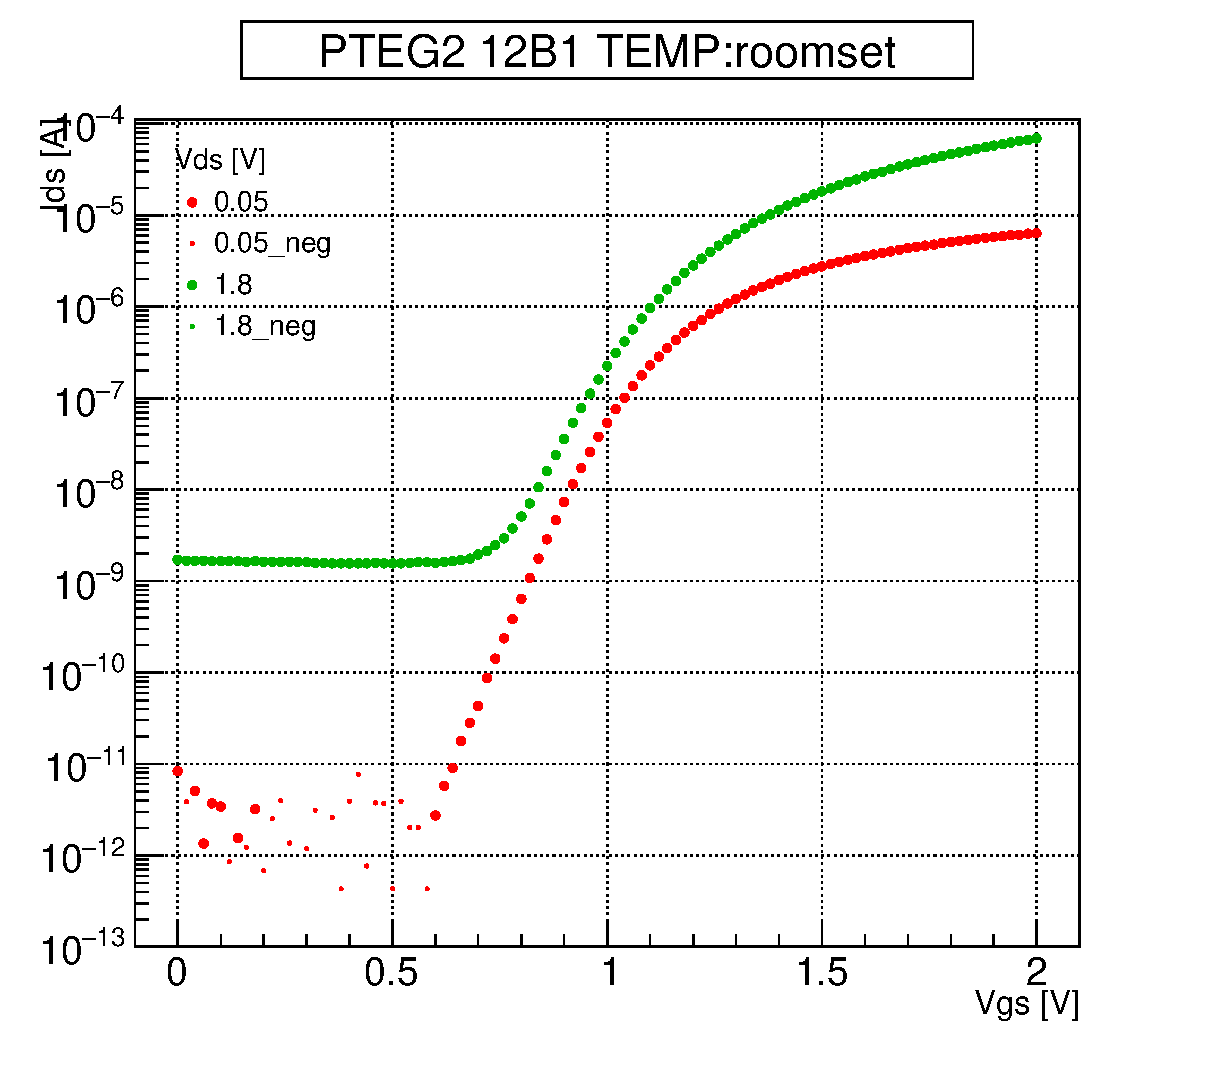
\includegraphics[width=70mm]{./Chapter/Appendix/Picture/NBT/B1/PTEG2_12_B1_IdVg_roomset.eps}
						\end{center}
						\caption{B1(W/L=$0.2\mathrm{\mu m}/0.4\mathrm{\mu m}$)の$I_{ds}-V_{gs}$特性(常温)}
						\label{fig:B1_IdVg_room}
					\end{minipage}
					\begin{minipage}{0.5\hsize}
						\begin{center}
							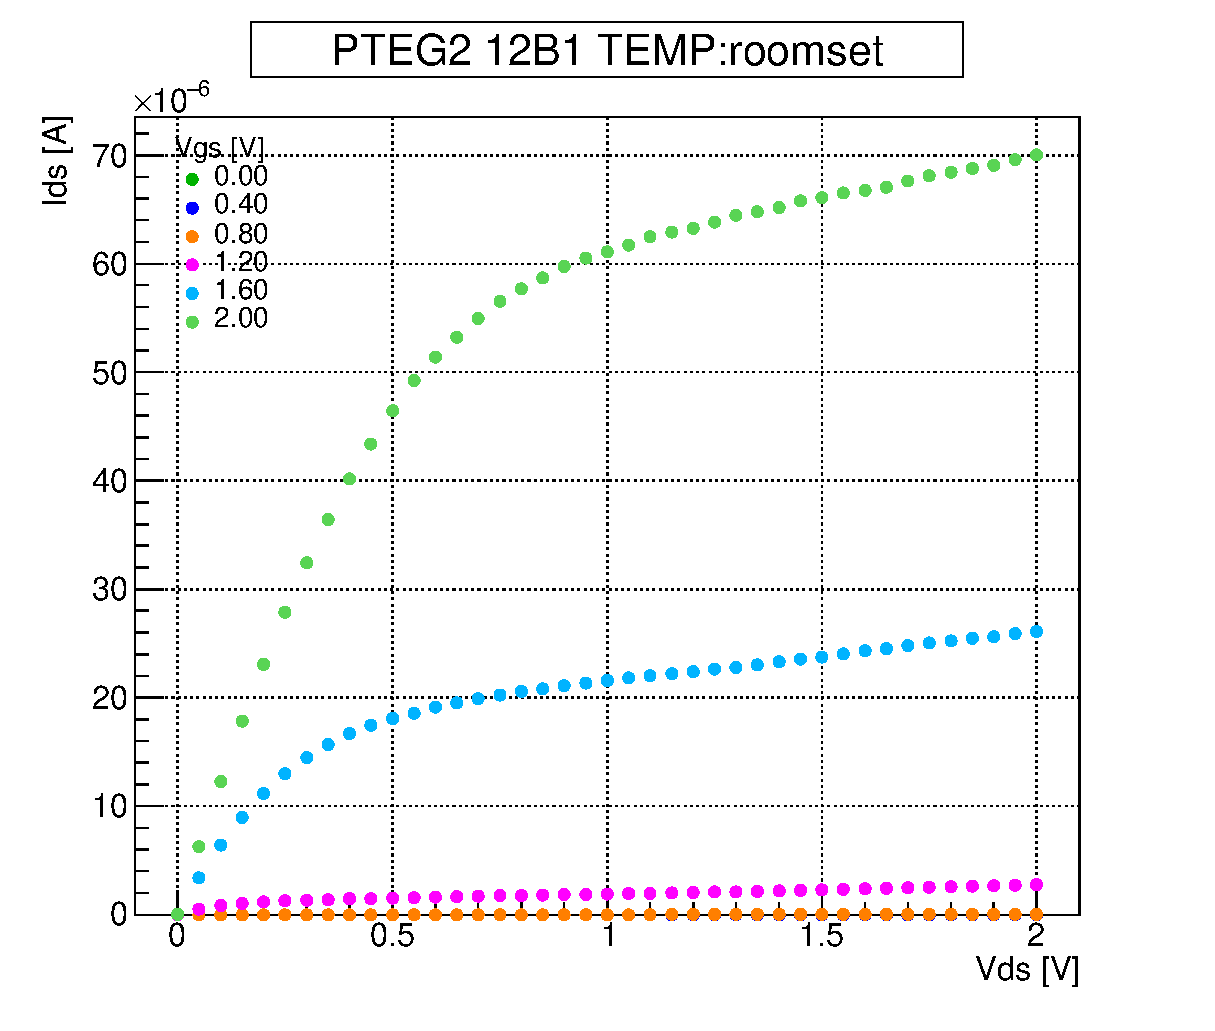
\includegraphics[width=70mm]{./Chapter/Appendix/Picture/NBT/B1/PTEG2_12_B1_IdVd_roomset.eps}
						\end{center}
						\caption{B1(W/L=$0.2\mathrm{\mu m}/0.4\mathrm{\mu m}$)の$I_{ds}-V_{ds}$特性(常温)}
						\label{fig:B1_IdVd_room}
					\end{minipage}
				\end{figure}
				%=====B2=====%
				\begin{figure}[htbp]
					\begin{minipage}{0.5\hsize}
						\begin{center}
							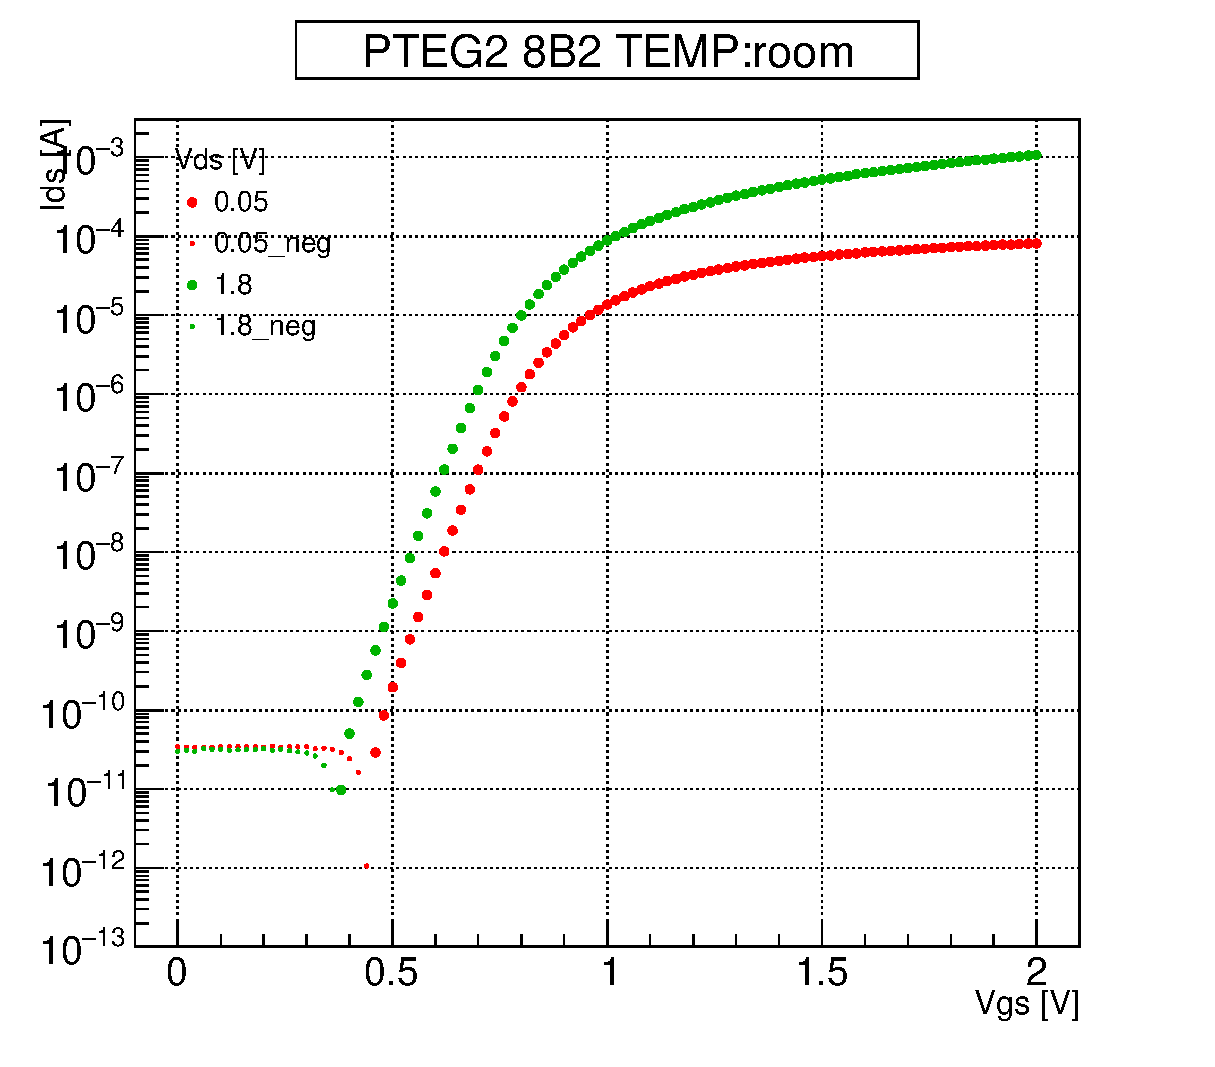
\includegraphics[width=70mm]{./Chapter/Appendix/Picture/NBT/B2/PTEG2_8_B2_IdVg_room.eps}
						\end{center}
						\caption{B2(W/L=$0.2\mathrm{\mu m}/5\mathrm{\mu m}$)の$I_{ds}-V_{gs}$特性(常温)}
						\label{fig:B2_IdVg_room}
					\end{minipage}
					\begin{minipage}{0.5\hsize}
						\begin{center}
							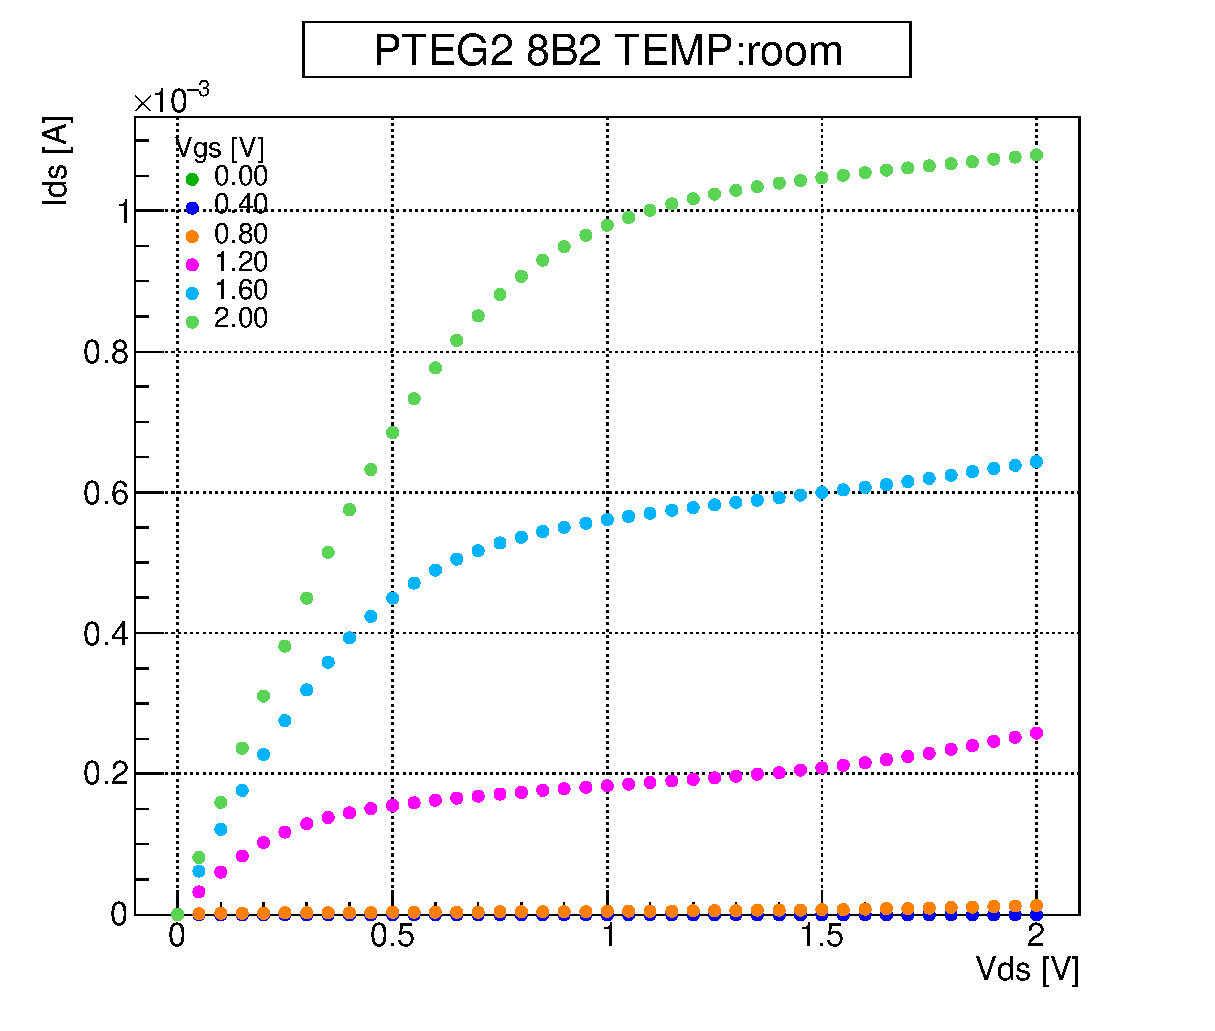
\includegraphics[width=70mm]{./Chapter/Appendix/Picture/NBT/B2/PTEG2_8_B2_IdVd_room.eps}
						\end{center}
						\caption{B2(W/L=$0.2\mathrm{\mu m}/5\mathrm{\mu m}$)の$I_{ds}-V_{ds}$特性(常温)}
						\label{fig:B2_IdVd_room}
					\end{minipage}
				\end{figure}
				%=====B3=====%
				\begin{figure}[htbp]
					\begin{minipage}{0.5\hsize}
						\begin{center}
							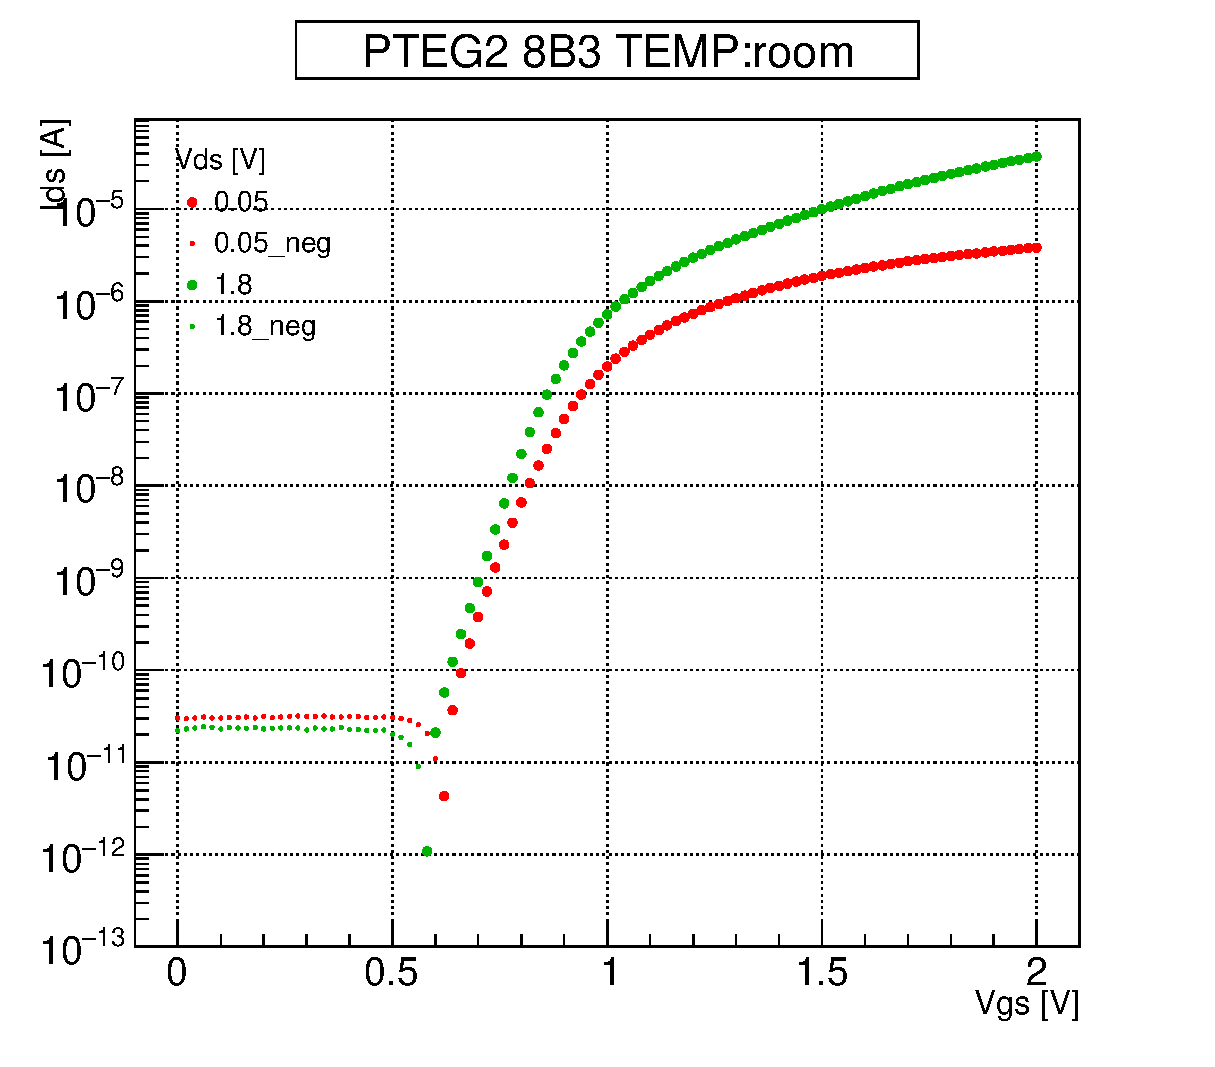
\includegraphics[width=70mm]{./Chapter/Appendix/Picture/NBT/B3/PTEG2_8_B3_IdVg_room.eps}
						\end{center}
						\caption{B3(W/L=$10\mathrm{\mu m}/5\mathrm{\mu m}$)の$I_{ds}-V_{gs}$特性(常温)}
						\label{fig:B3_IdVg_room}
					\end{minipage}
					\begin{minipage}{0.5\hsize}
						\begin{center}
							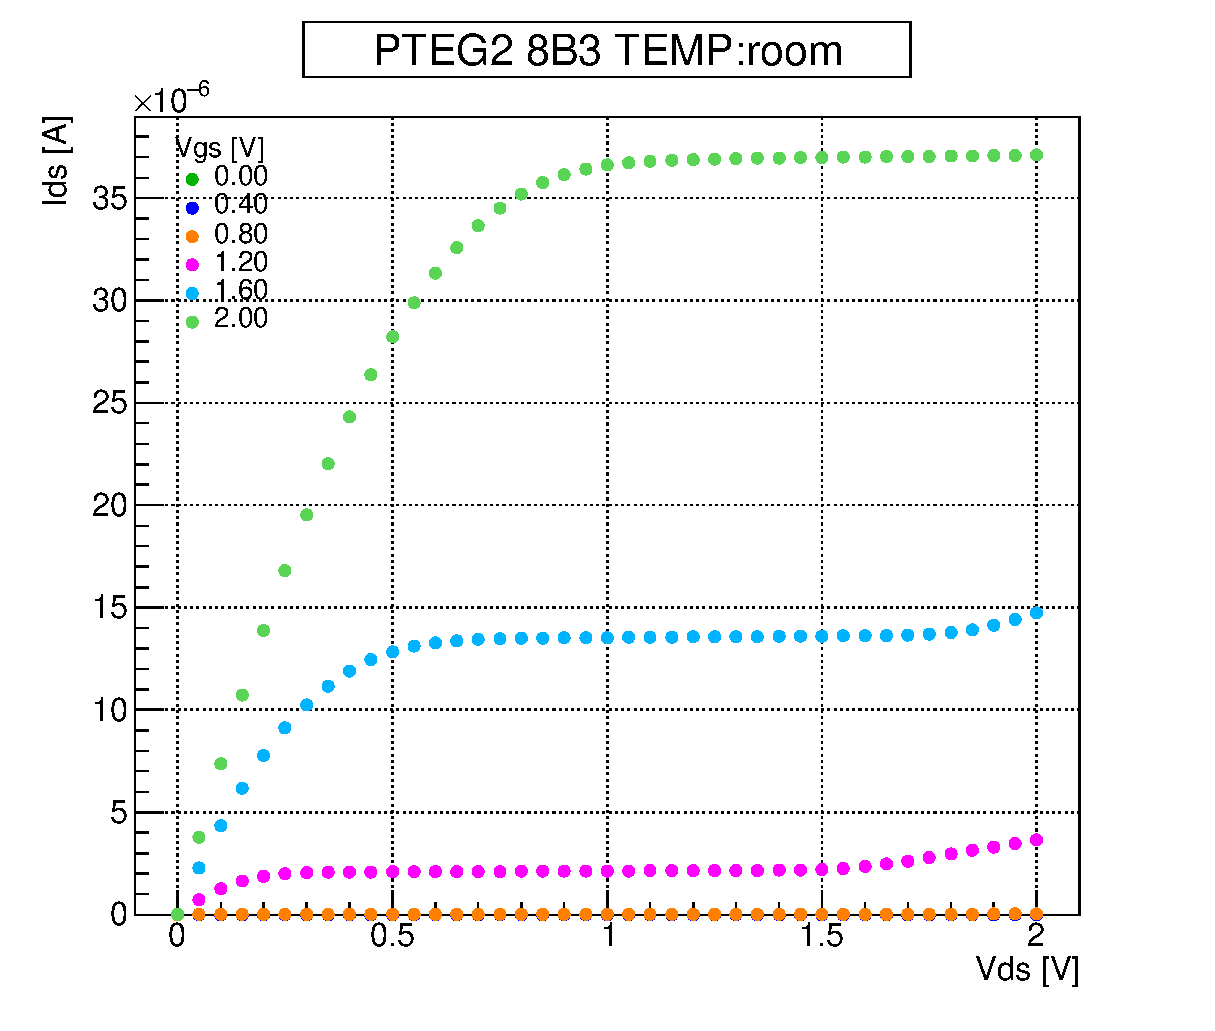
\includegraphics[width=70mm]{./Chapter/Appendix/Picture/NBT/B3/PTEG2_8_B3_IdVd_room.eps}
						\end{center}
						\caption{B3(W/L=$10\mathrm{\mu m}/5\mathrm{\mu m}$)の$I_{ds}-V_{ds}$特性(常温)}
						\label{fig:B3_IdVd_room}
					\end{minipage}
				\end{figure}
				%=====B4=====%
				\begin{figure}[htbp]
					\begin{minipage}{0.5\hsize}
						\begin{center}
							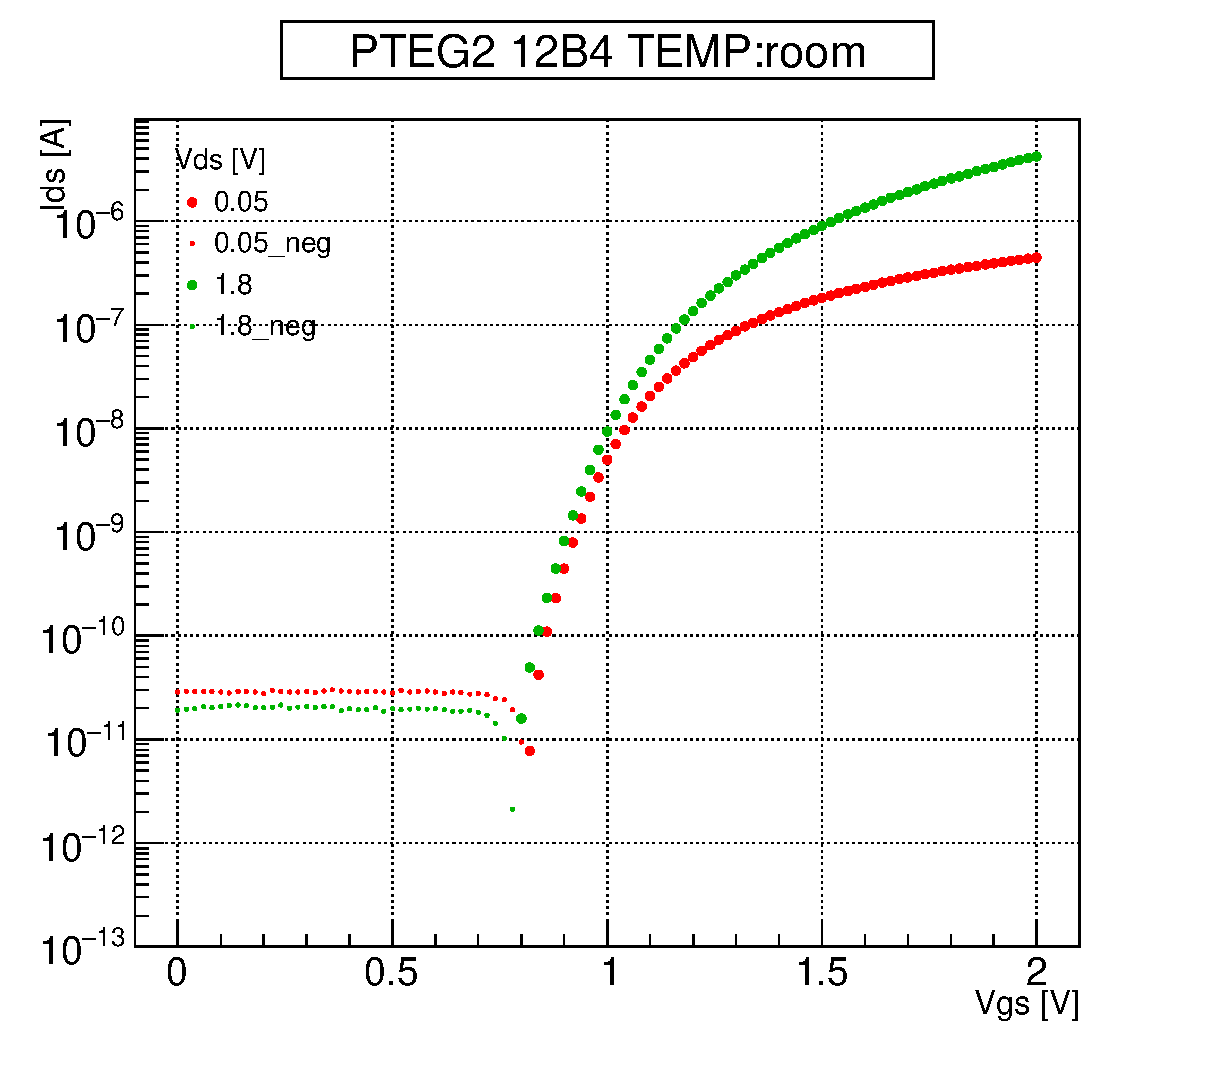
\includegraphics[width=70mm]{./Chapter/Appendix/Picture/NBT/B4/PTEG2_12_B4_IdVg_room.eps}
						\end{center}
						\caption{B4(W/L=$10\mathrm{\mu m}/0.4\mathrm{\mu m}$)の$I_{ds}-V_{gs}$特性(常温)}
						\label{fig:B4_IdVg_room}
					\end{minipage}
					\begin{minipage}{0.5\hsize}
						\begin{center}
							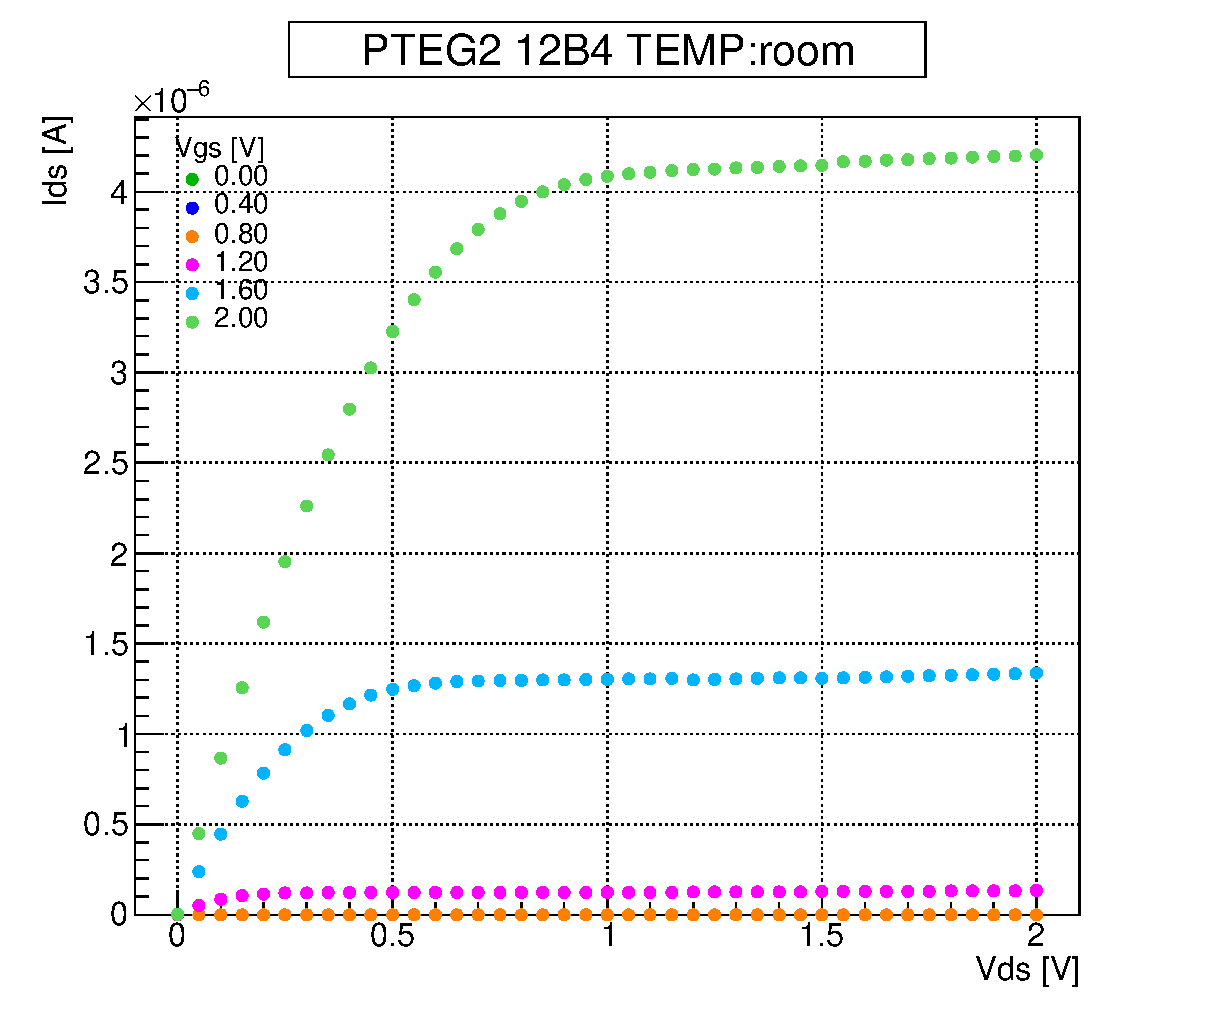
\includegraphics[width=70mm]{./Chapter/Appendix/Picture/NBT/B4/PTEG2_12_B4_IdVd_room.eps}
						\end{center}
						\caption{B4(W/L=$10\mathrm{\mu m}/0.4\mathrm{\mu m}$)の$I_{ds}-V_{ds}$特性(常温)}
						\label{fig:B4_IdVd_room}
					\end{minipage}
				\end{figure}
				\clearpage
		\section{NMOS-BT(3K環境下)}
				%=====B1=====%
				\begin{figure}[htbp]
					\begin{minipage}{0.5\hsize}
						\begin{center}
							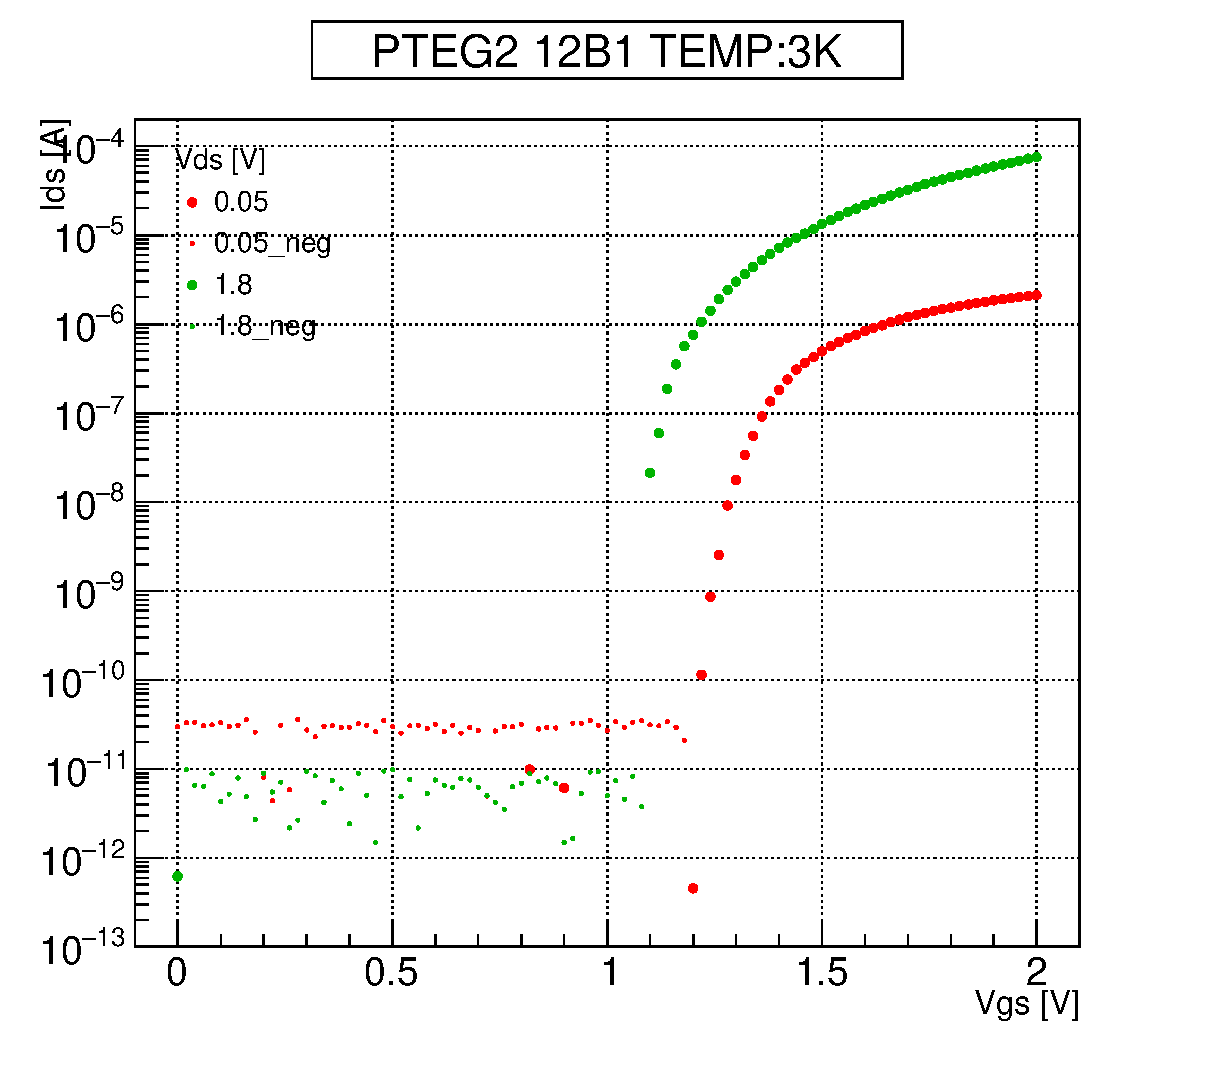
\includegraphics[width=70mm]{./Chapter/Appendix/Picture/NBT/B1/PTEG2_12_B1_IdVg_3K.eps}
						\end{center}
						\caption{B1(W/L=$0.2\mathrm{\mu m}/0.4\mathrm{\mu m}$)の$I_{ds}-V_{gs}$特性(3K)}
						\label{fig:B1_IdVg_3K}
					\end{minipage}
					\begin{minipage}{0.5\hsize}
						\begin{center}
							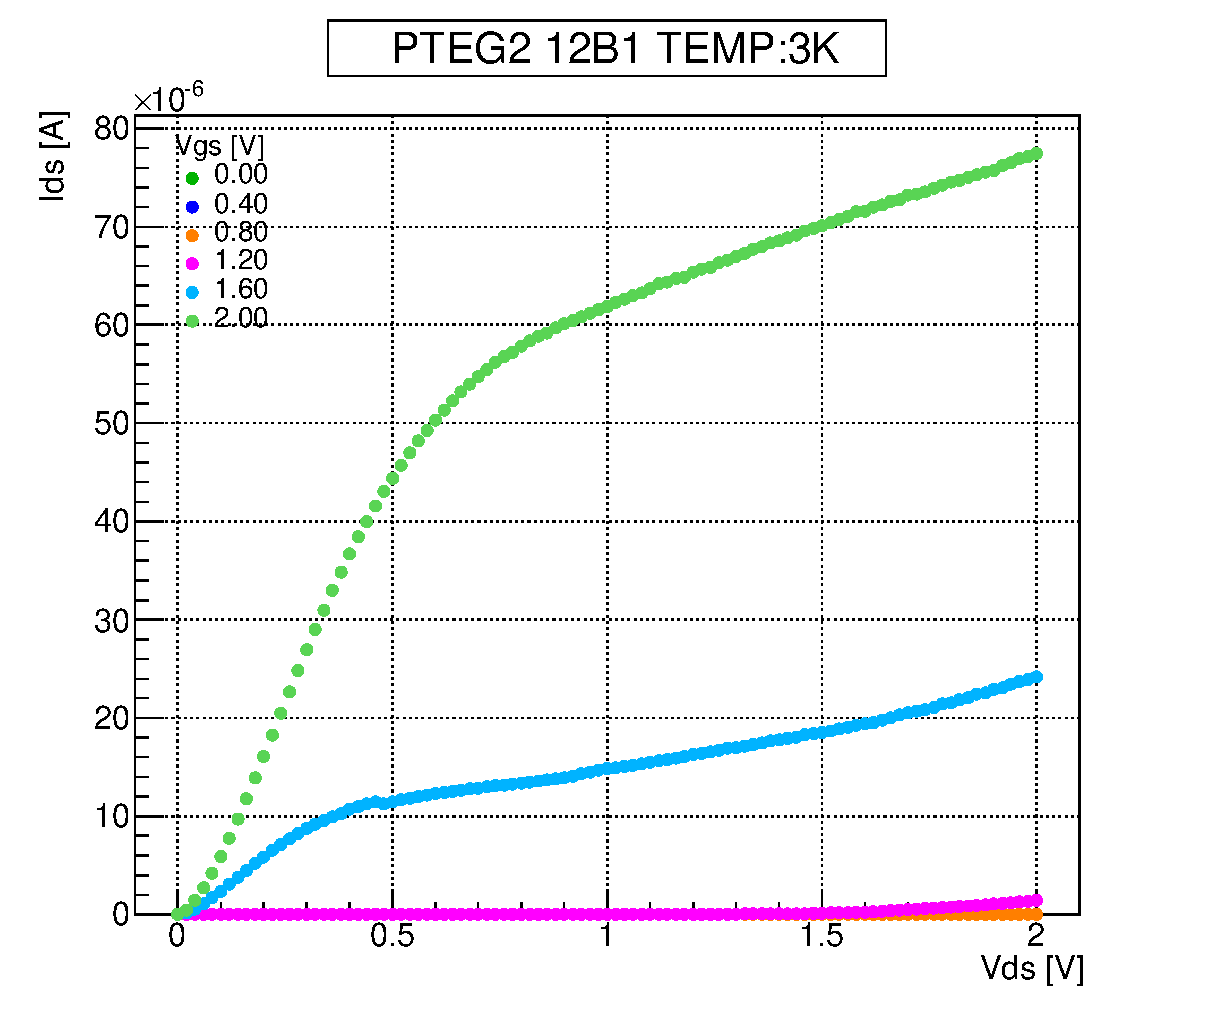
\includegraphics[width=70mm]{./Chapter/Appendix/Picture/NBT/B1/PTEG2_12_B1_IdVd_3K.eps}
						\end{center}
						\caption{B1(W/L=$0.2\mathrm{\mu m}/0.4\mathrm{\mu m}$)の$I_{ds}-V_{ds}$特性(3K)}
						\label{fig:B1_IdVd_3K}
					\end{minipage}
				\end{figure}
				%=====B2=====%
				\begin{figure}[htbp]
					\begin{minipage}{0.5\hsize}
						\begin{center}
							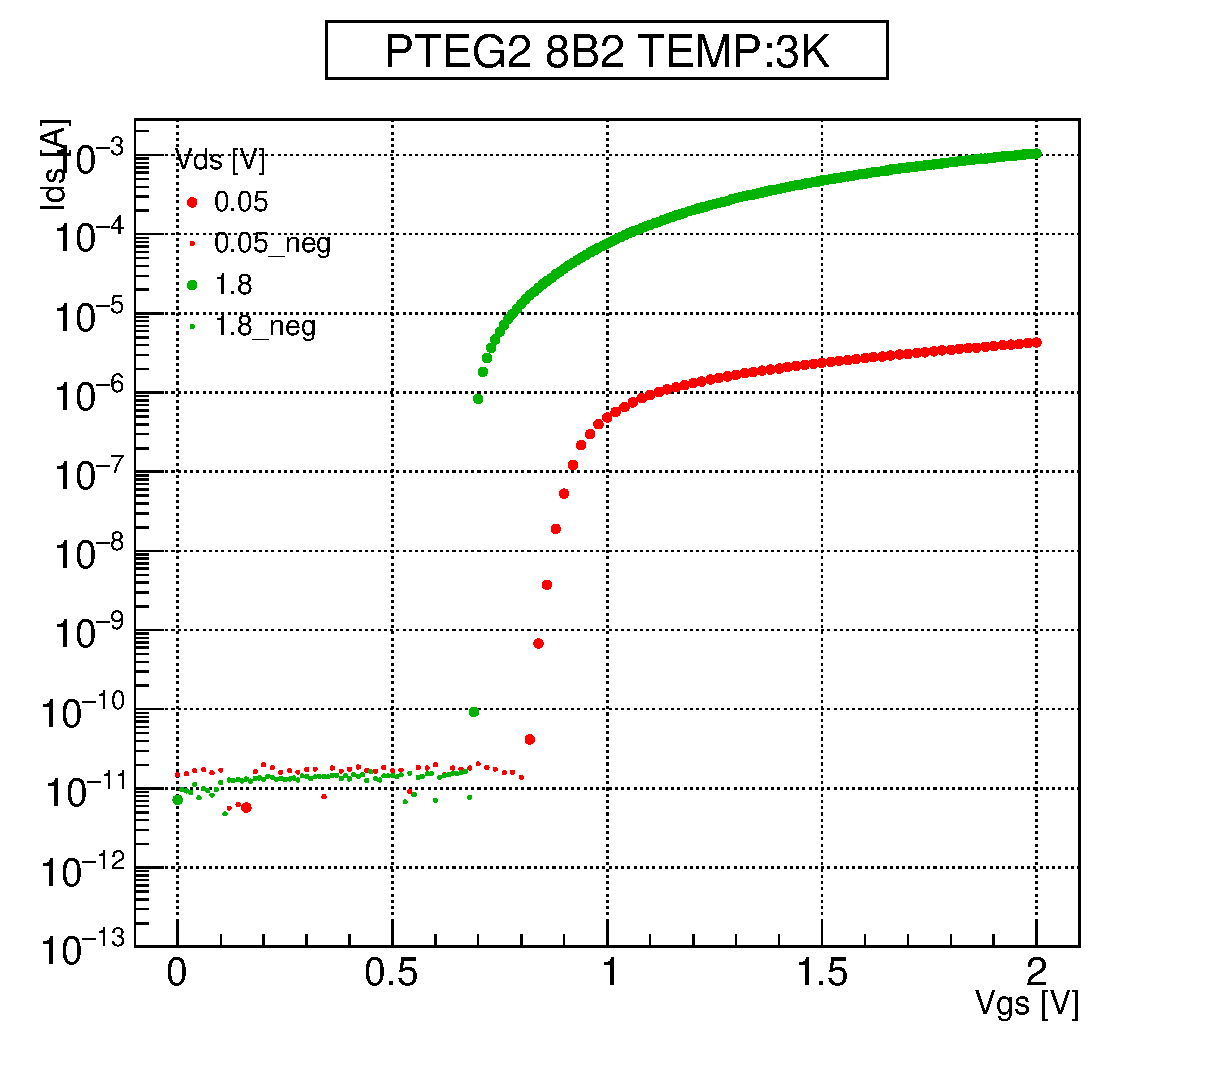
\includegraphics[width=70mm]{./Chapter/Appendix/Picture/NBT/B2/PTEG2_8_B2_IdVg_3K.eps}
						\end{center}
						\caption{B2(W/L=$0.2\mathrm{\mu m}/5\mathrm{\mu m}$)の$I_{ds}-V_{gs}$特性(3K)}
						\label{fig:B2_IdVg_3K}
					\end{minipage}
					\begin{minipage}{0.5\hsize}
						\begin{center}
							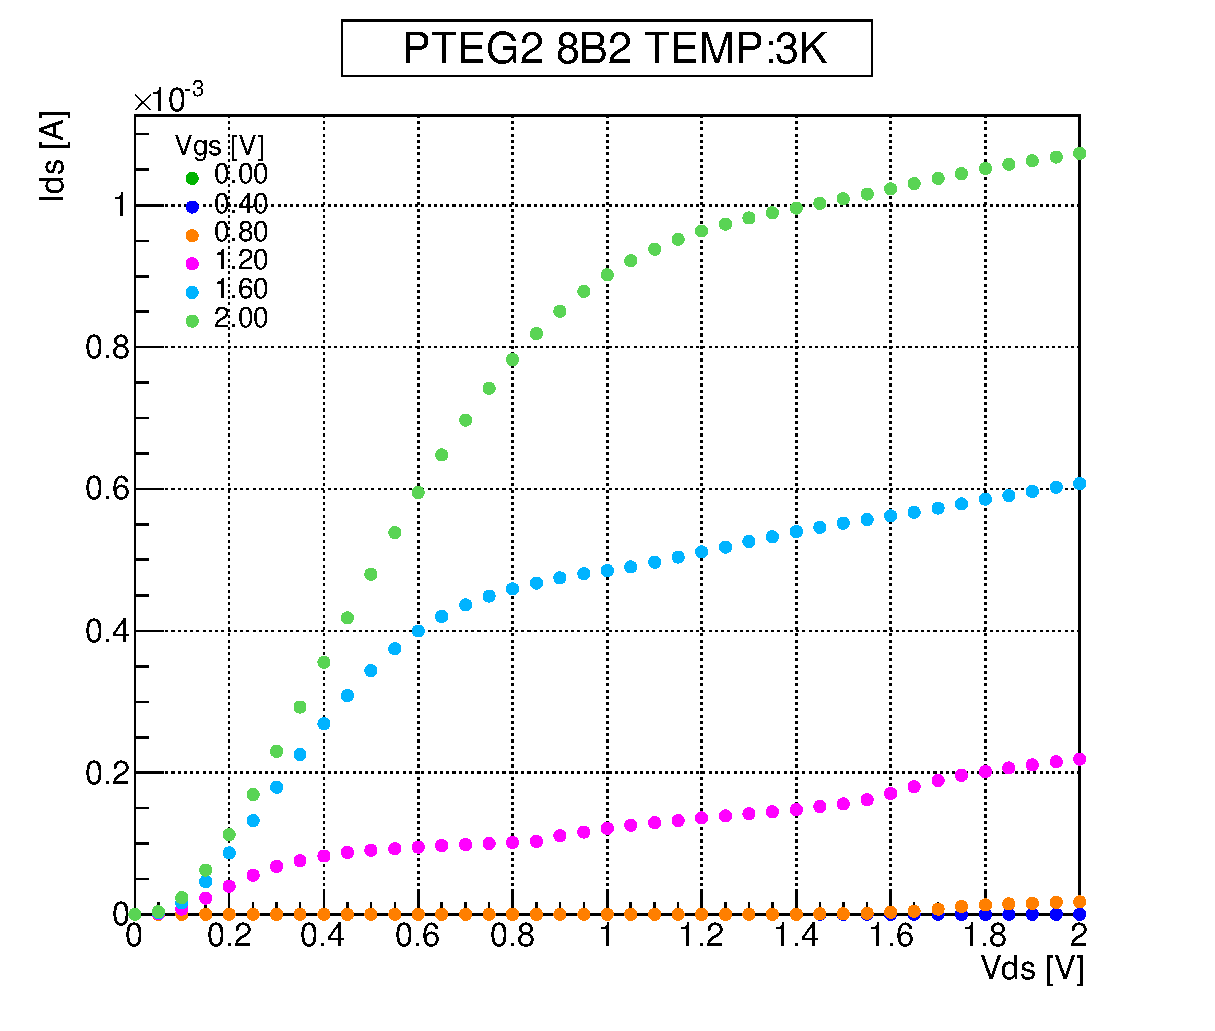
\includegraphics[width=70mm]{./Chapter/Appendix/Picture/NBT/B2/PTEG2_8_B2_IdVd_3K.eps}
						\end{center}
						\caption{B2(W/L=$0.2\mathrm{\mu m}/5\mathrm{\mu m}$)の$I_{ds}-V_{ds}$特性(3K)}
						\label{fig:B2_IdVd_3K}
					\end{minipage}
				\end{figure}
				%=====B3=====%
				\begin{figure}[htbp]
					\begin{minipage}{0.5\hsize}
						\begin{center}
							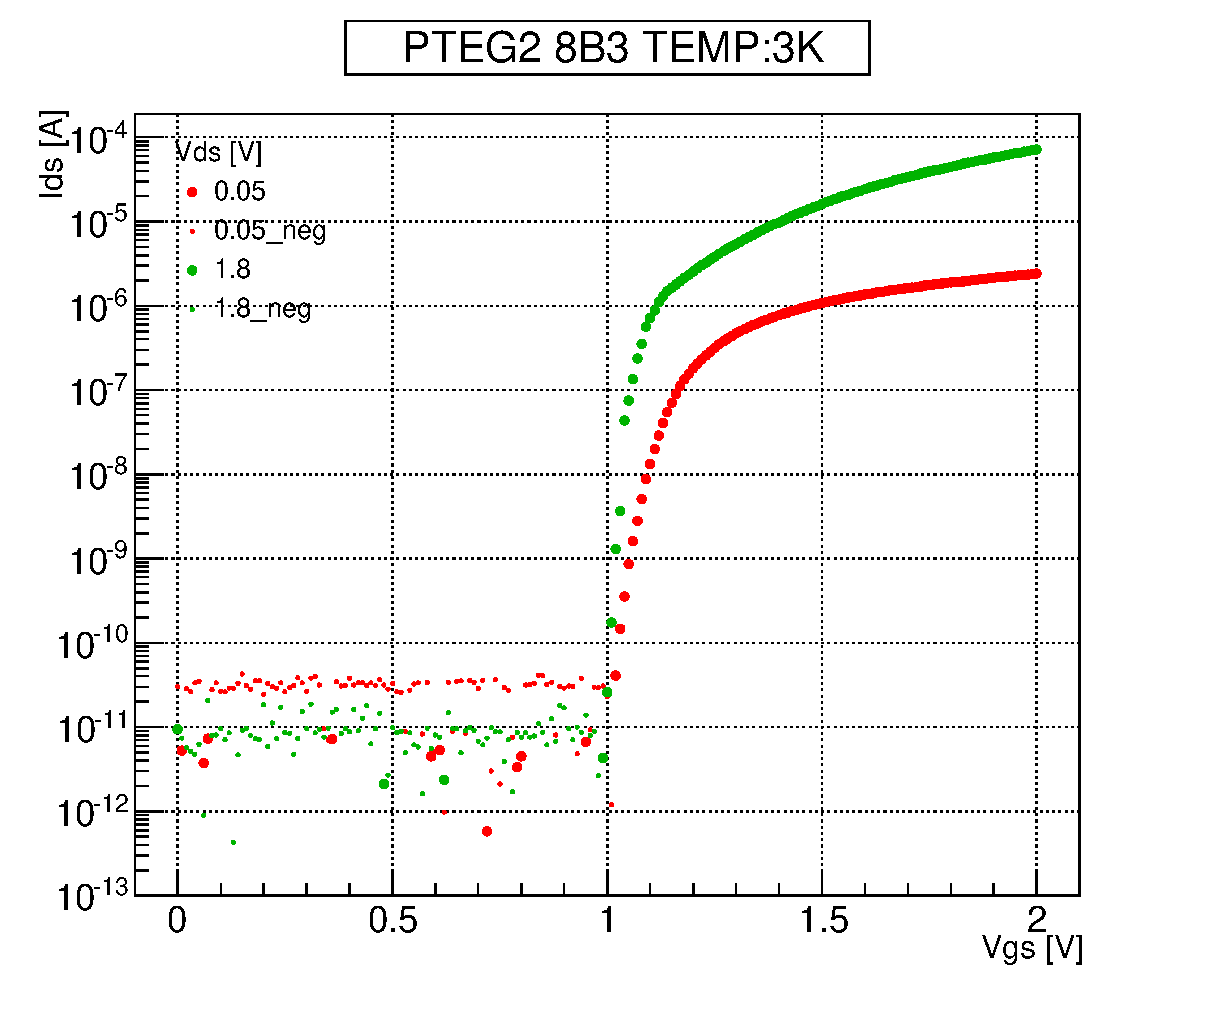
\includegraphics[width=70mm]{./Chapter/Appendix/Picture/NBT/B3/PTEG2_8_B3_IdVg_3K.eps}
						\end{center}
						\caption{B3(W/L=$10\mathrm{\mu m}/5\mathrm{\mu m}$)の$I_{ds}-V_{gs}$特性(3K)}
						\label{fig:B3_IdVg_3K}
					\end{minipage}
					\begin{minipage}{0.5\hsize}
						\begin{center}
							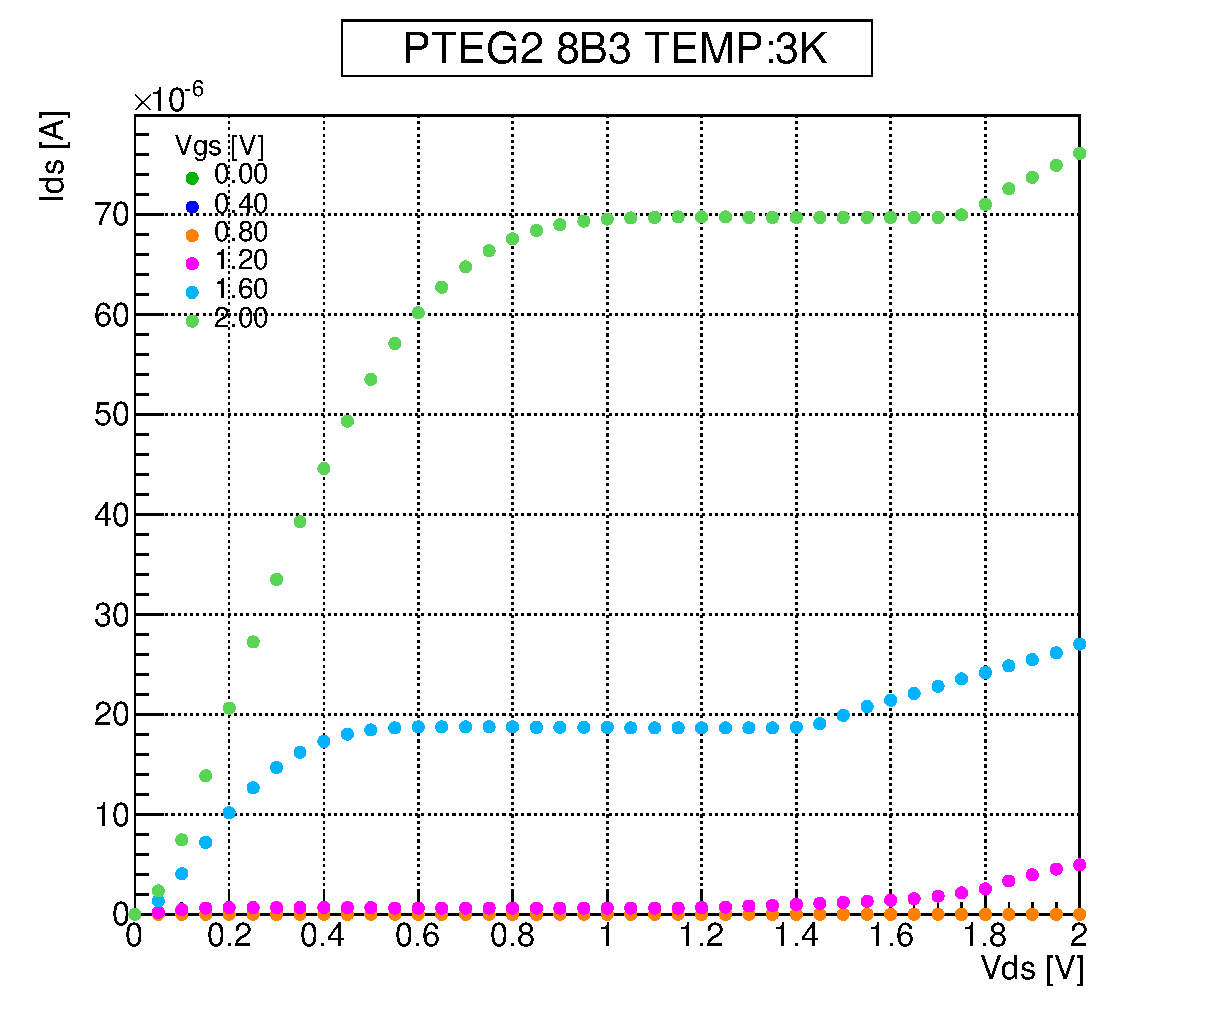
\includegraphics[width=70mm]{./Chapter/Appendix/Picture/NBT/B3/PTEG2_8_B3_IdVd_3K.eps}
						\end{center}
						\caption{B3(W/L=$10\mathrm{\mu m}/5\mathrm{\mu m}$)の$I_{ds}-V_{ds}$特性(3K)}
						\label{fig:B3_IdVd_3K}
					\end{minipage}
				\end{figure}
				%=====B4=====%
				\begin{figure}[htbp]
					\begin{minipage}{0.5\hsize}
						\begin{center}
							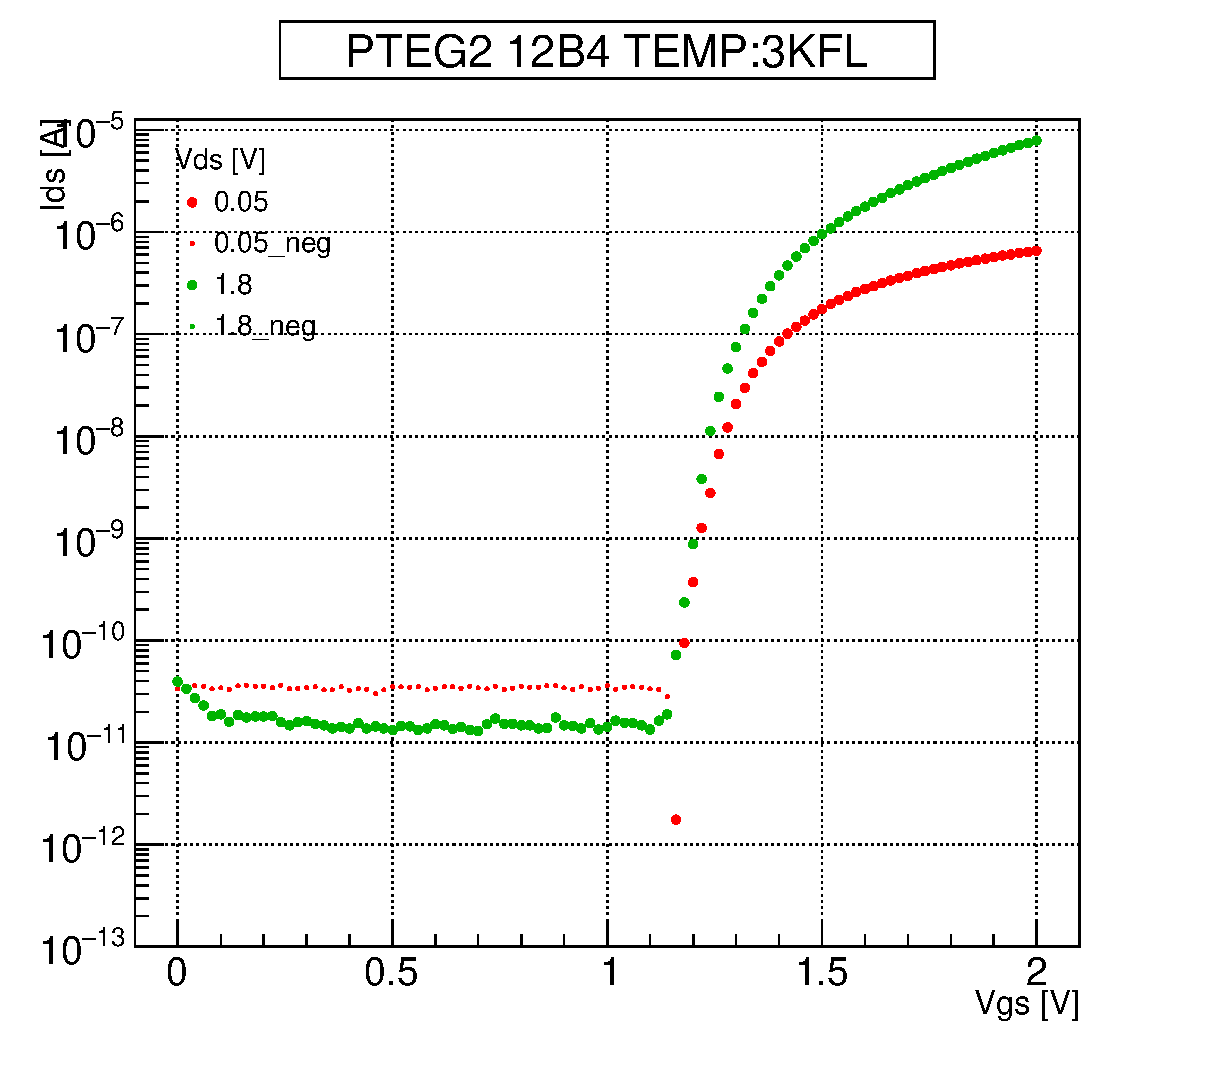
\includegraphics[width=70mm]{./Chapter/Appendix/Picture/NBT/B4/PTEG2_12_B4_IdVg_3KFL.eps}
						\end{center}
						\caption{B4(W/L=$10\mathrm{\mu m}/0.4\mathrm{\mu m}$)の$I_{ds}-V_{gs}$特性(3K)}
						\label{fig:B4_IdVg_3K}
					\end{minipage}
					\begin{minipage}{0.5\hsize}
						\begin{center}
							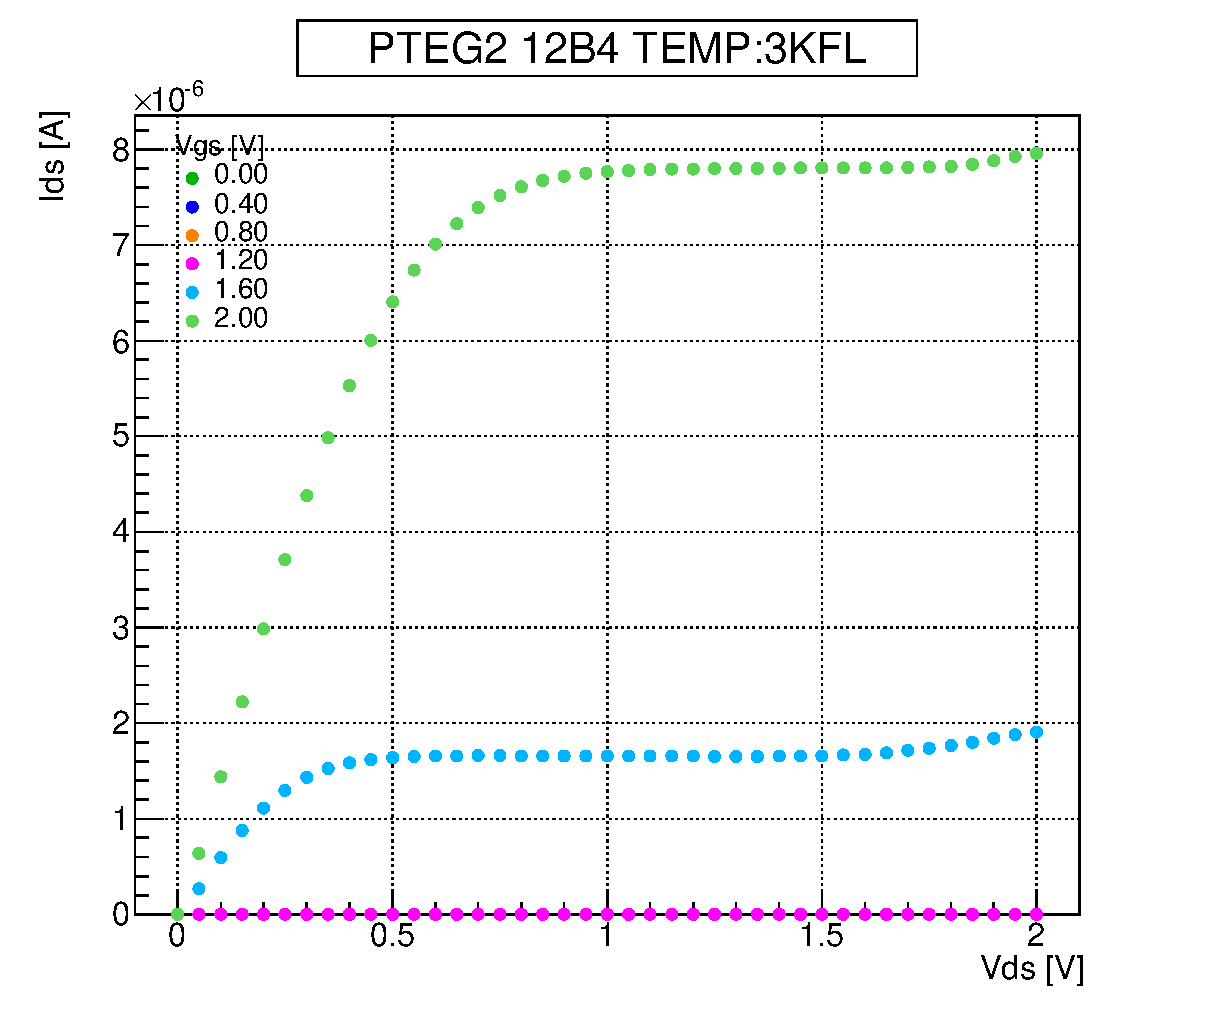
\includegraphics[width=70mm]{./Chapter/Appendix/Picture/NBT/B4/PTEG2_12_B4_IdVd_3KFL.eps}
						\end{center}
						\caption{B4(W/L=$10\mathrm{\mu m}/0.4\mathrm{\mu m}$)の$I_{ds}-V_{ds}$特性(3K)}
						\label{fig:B4_IdVd_3K}
					\end{minipage}
				\end{figure}
				\clearpage
		\section{PMOS-BT(常温環境下)}
				%=====B5=====%
				\begin{figure}[htbp]
					\begin{minipage}{0.5\hsize}
						\begin{center}
							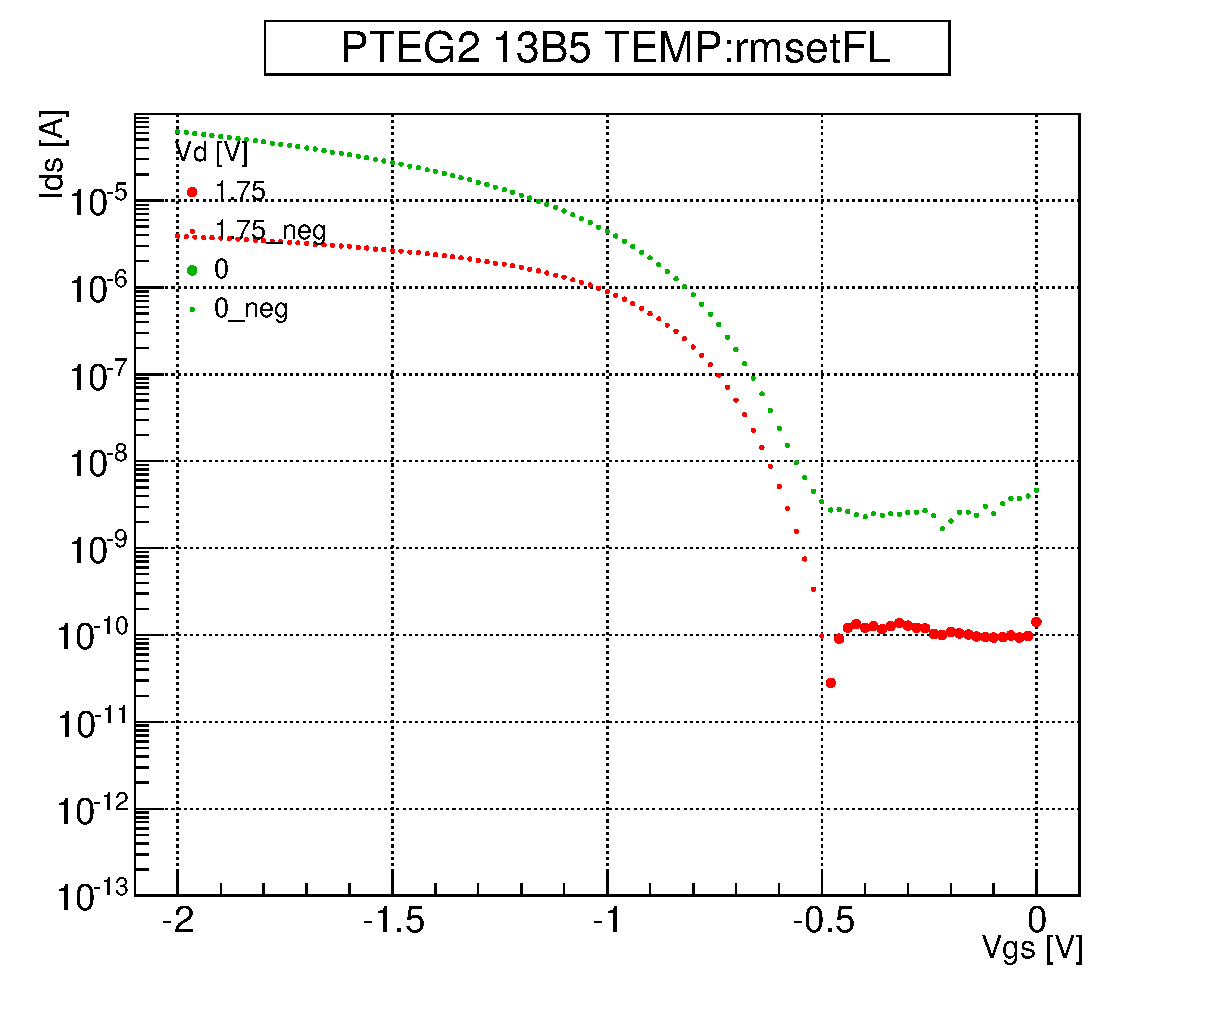
\includegraphics[width=70mm]{./Chapter/Appendix/Picture/PBT/B5/PTEG2_13_B5_IdVg_rmsetFL.eps}
						\end{center}
						\caption{B5(W/L=$0.2\mathrm{\mu m}/0.5\mathrm{\mu m}$)の$I_{ds}-V_{gs}$特性(常温)}
						\label{fig:B5_IdVg_room}
					\end{minipage}
					\begin{minipage}{0.5\hsize}
						\begin{center}
							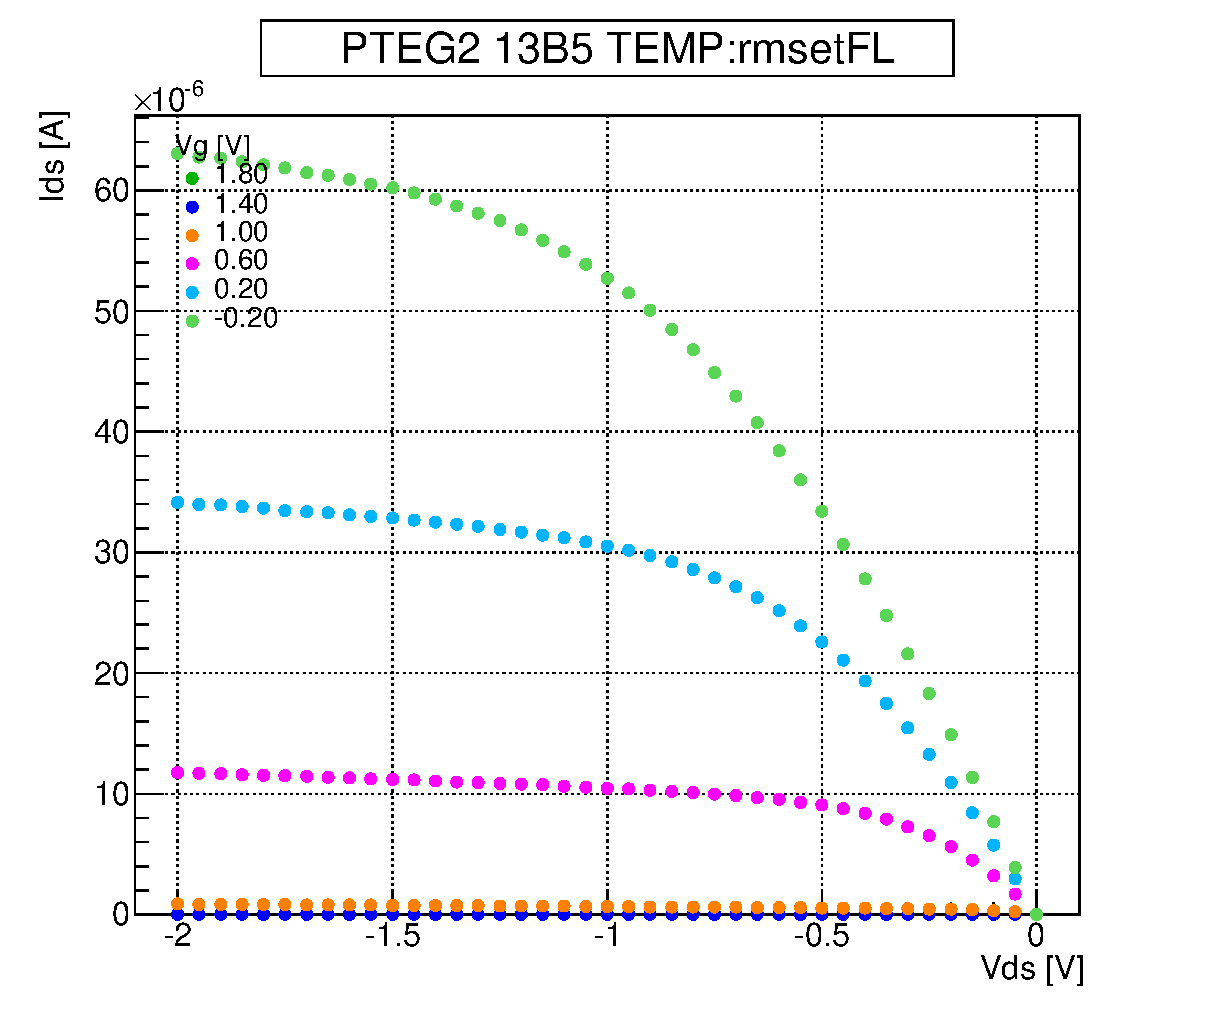
\includegraphics[width=70mm]{./Chapter/Appendix/Picture/PBT/B5/PTEG2_13_B5_IdVd_rmsetFL.eps}
						\end{center}
						\caption{B5(W/L=$0.2\mathrm{\mu m}/0.5\mathrm{\mu m}$)の$I_{ds}-V_{ds}$特性(常温)}
						\label{fig:B5_IdVd_room}
					\end{minipage}
				\end{figure}
				%=====B6=====%
				\begin{figure}[htbp]
					\begin{minipage}{0.5\hsize}
						\begin{center}
							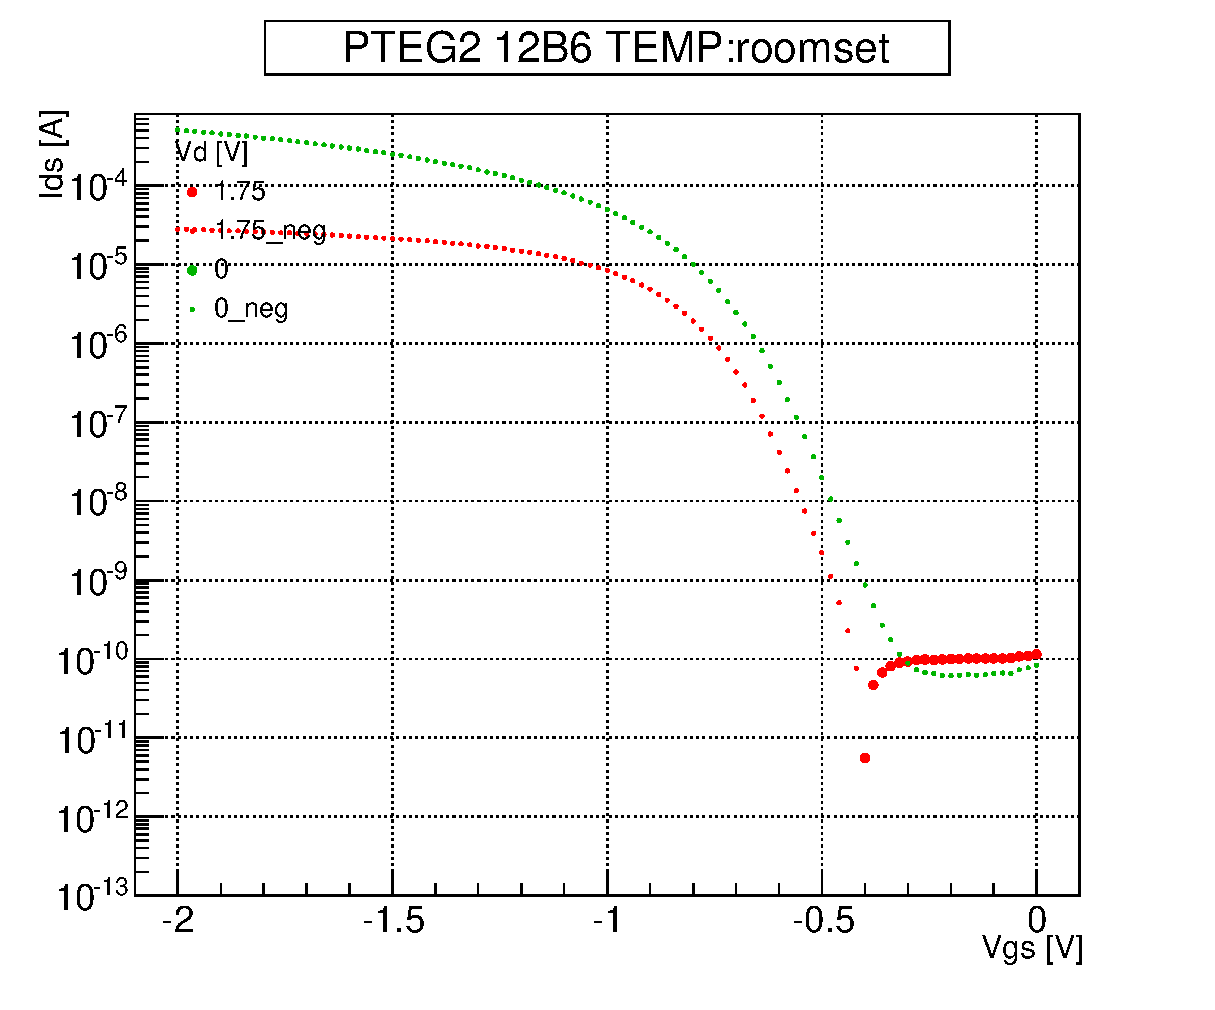
\includegraphics[width=70mm]{./Chapter/Appendix/Picture/PBT/B6/PTEG2_12_B6_IdVg_roomset.eps}
						\end{center}
						\caption{B6(W/L=$0.2\mathrm{\mu m}/5\mathrm{\mu m}$)の$I_{ds}-V_{gs}$特性(常温)}
						\label{fig:B6_IdVg_room}
					\end{minipage}
					\begin{minipage}{0.5\hsize}
						\begin{center}
							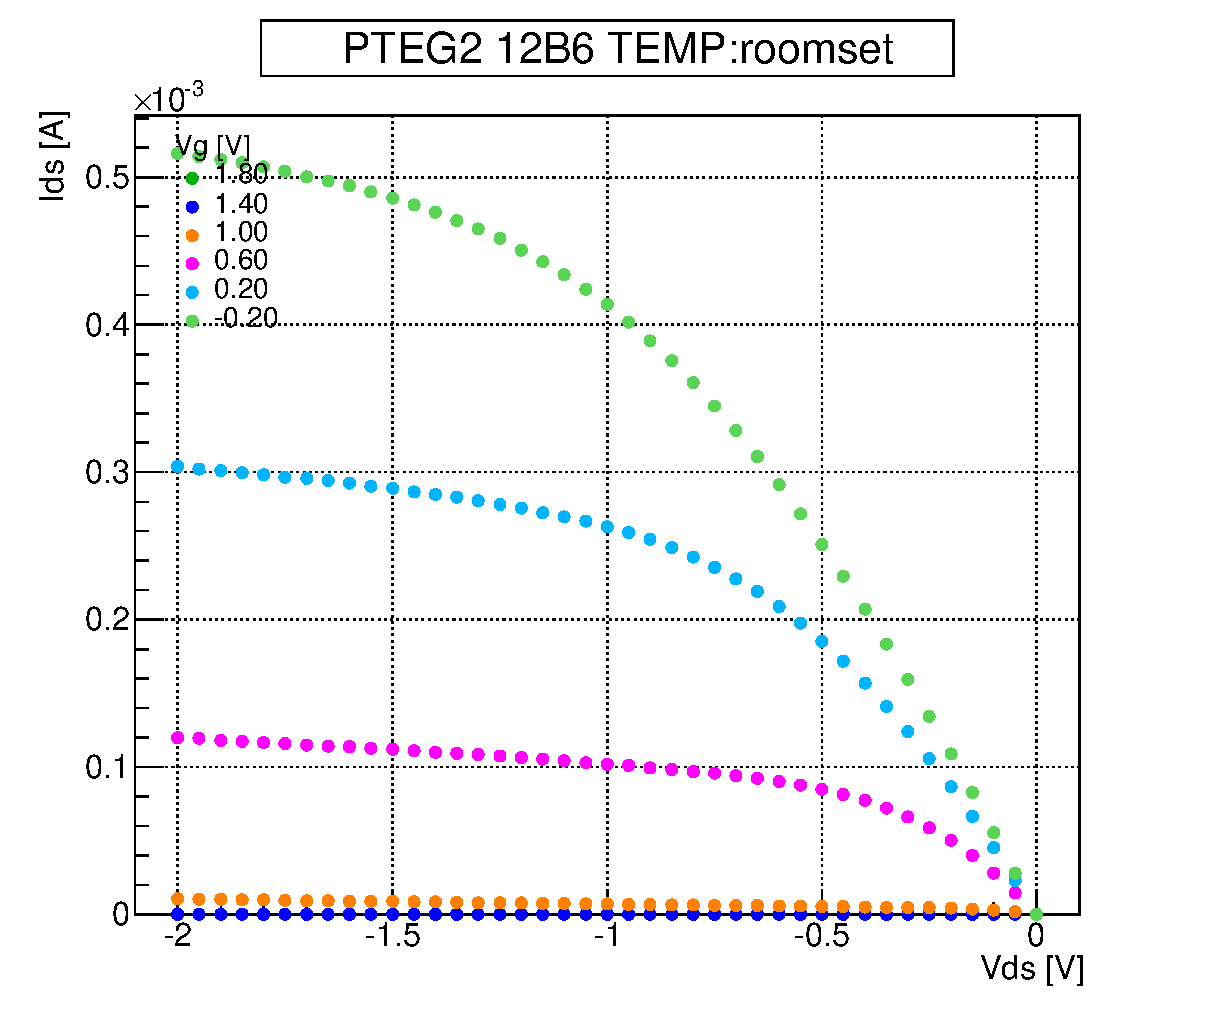
\includegraphics[width=70mm]{./Chapter/Appendix/Picture/PBT/B6/PTEG2_12_B6_IdVd_roomset.eps}
						\end{center}
						\caption{B6(W/L=$0.2\mathrm{\mu m}/5\mathrm{\mu m}$)の$I_{ds}-V_{ds}$特性(常温)}
						\label{fig:B6_IdVd_room}
					\end{minipage}
				\end{figure}
				%=====B7=====%
				\begin{figure}[htbp]
					\begin{minipage}{0.5\hsize}
						\begin{center}
							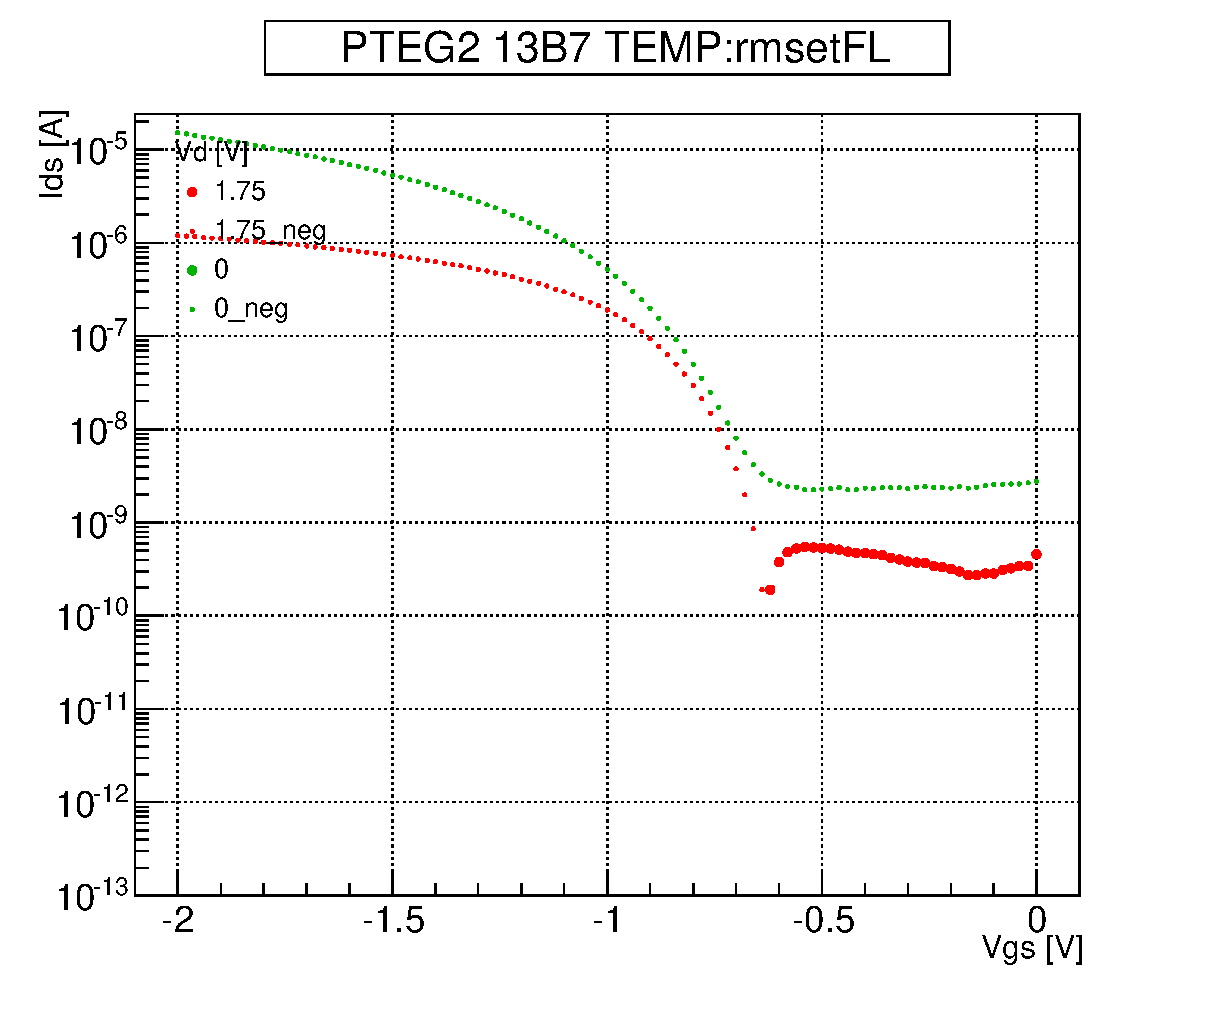
\includegraphics[width=70mm]{./Chapter/Appendix/Picture/PBT/B7/PTEG2_13_B7_IdVg_rmsetFL.eps}
						\end{center}
						\caption{B7(W/L=$10\mathrm{\mu m}/5\mathrm{\mu m}$)の$I_{ds}-V_{gs}$特性(常温)}
						\label{fig:B7_IdVg_room}
					\end{minipage}
					\begin{minipage}{0.5\hsize}
						\begin{center}
							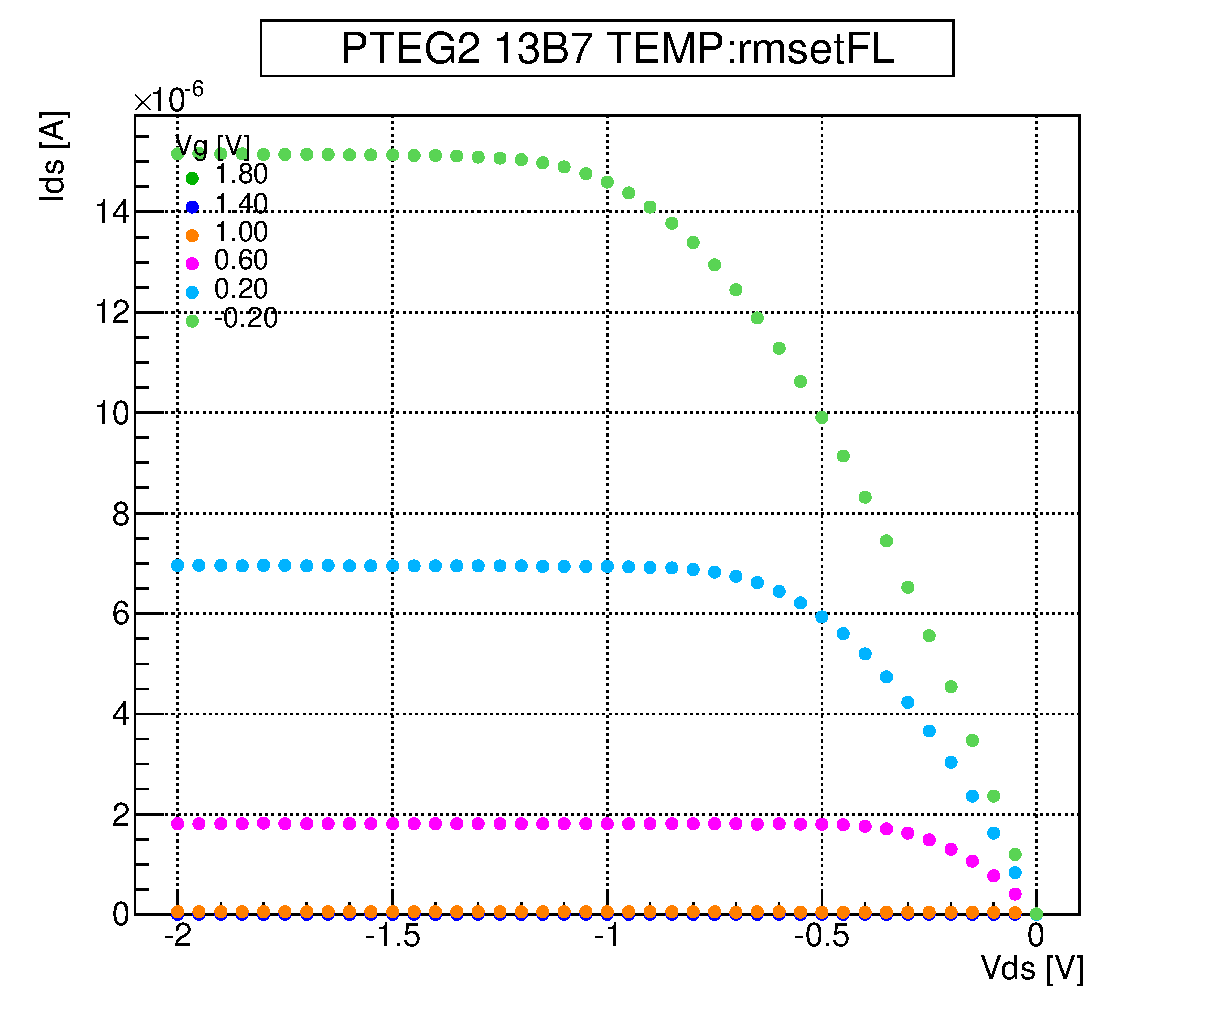
\includegraphics[width=70mm]{./Chapter/Appendix/Picture/PBT/B7/PTEG2_13_B7_IdVd_rmsetFL.eps}
						\end{center}
						\caption{B7(W/L=$10\mathrm{\mu m}/5\mathrm{\mu m}$)の$I_{ds}-V_{ds}$特性(常温)}
						\label{fig:B7_IdVd_room}
					\end{minipage}
				\end{figure}
				%=====B8=====%
				\begin{figure}[htbp]
					\begin{minipage}{0.5\hsize}
						\begin{center}
							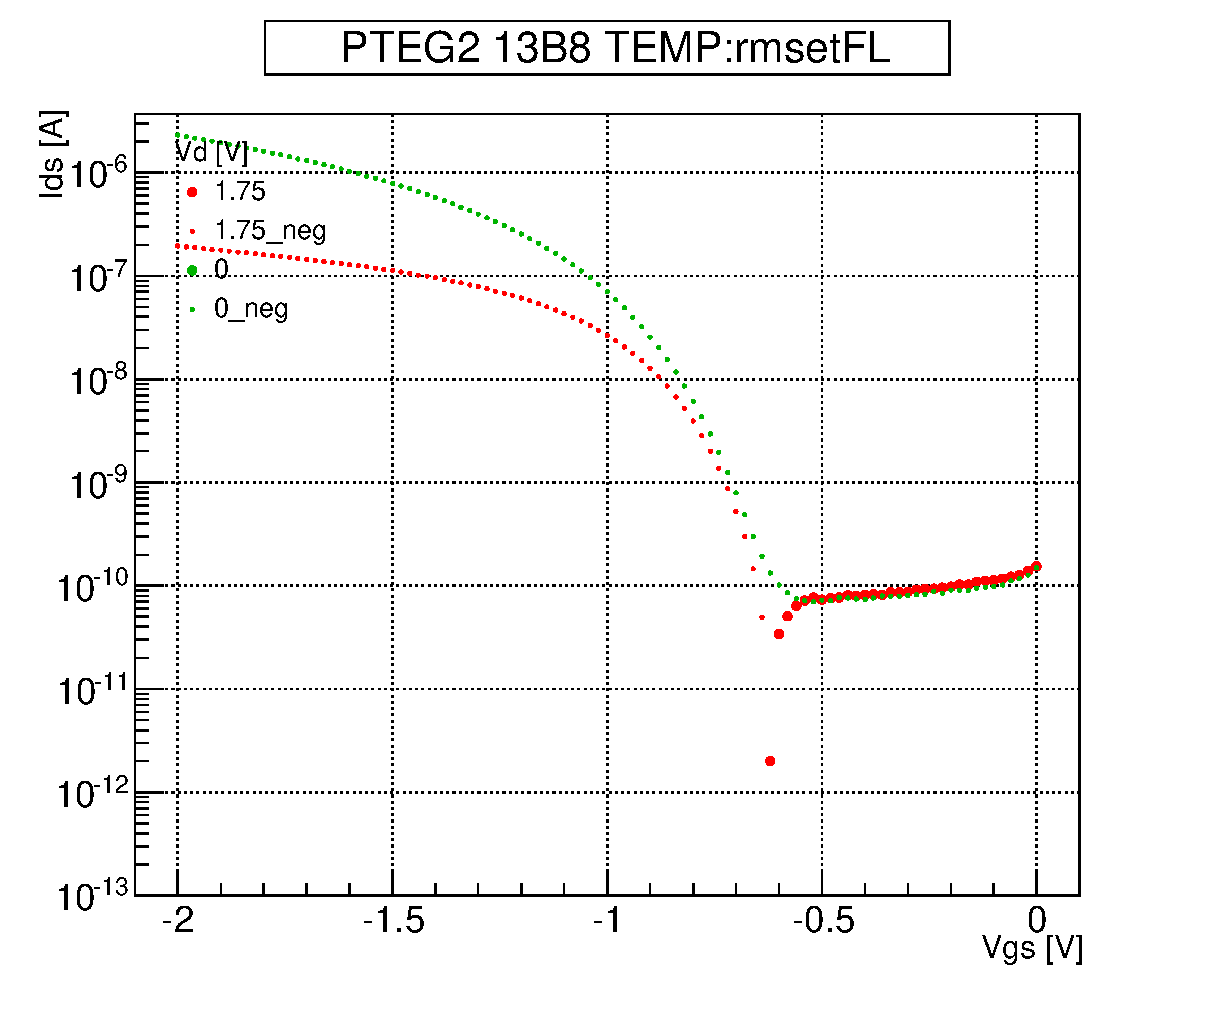
\includegraphics[width=70mm]{./Chapter/Appendix/Picture/PBT/B8/PTEG2_13_B8_IdVg_rmsetFL.eps}
						\end{center}
						\caption{B8(W/L=$10\mathrm{\mu m}/0.63\mathrm{\mu m}$)の$I_{ds}-V_{gs}$特性(常温)}
						\label{fig:B8_IdVg_room}
					\end{minipage}
					\begin{minipage}{0.5\hsize}
						\begin{center}
							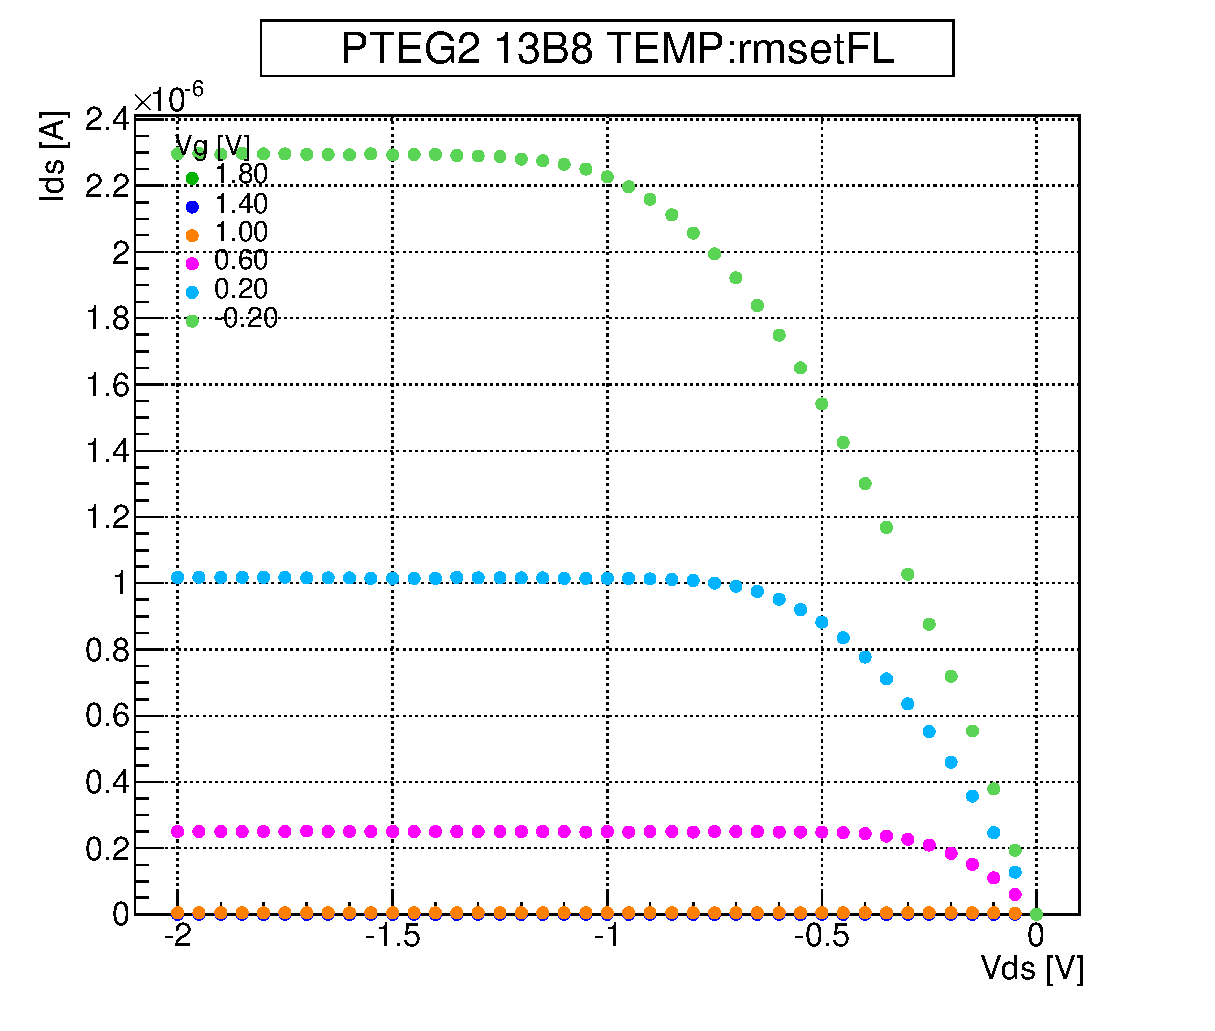
\includegraphics[width=70mm]{./Chapter/Appendix/Picture/PBT/B8/PTEG2_13_B8_IdVd_rmsetFL.eps}
						\end{center}
						\caption{B8(W/L=$10\mathrm{\mu m}/0.63\mathrm{\mu m}$)の$I_{ds}-V_{ds}$特性(常温)}
						\label{fig:B8_IdVd_room}
					\end{minipage}
				\end{figure}
				\clearpage
		\section{PMOS-BT(3K環境下)}
				%=====B5=====%
				\begin{figure}[htbp]
					\begin{minipage}{0.5\hsize}
						\begin{center}
							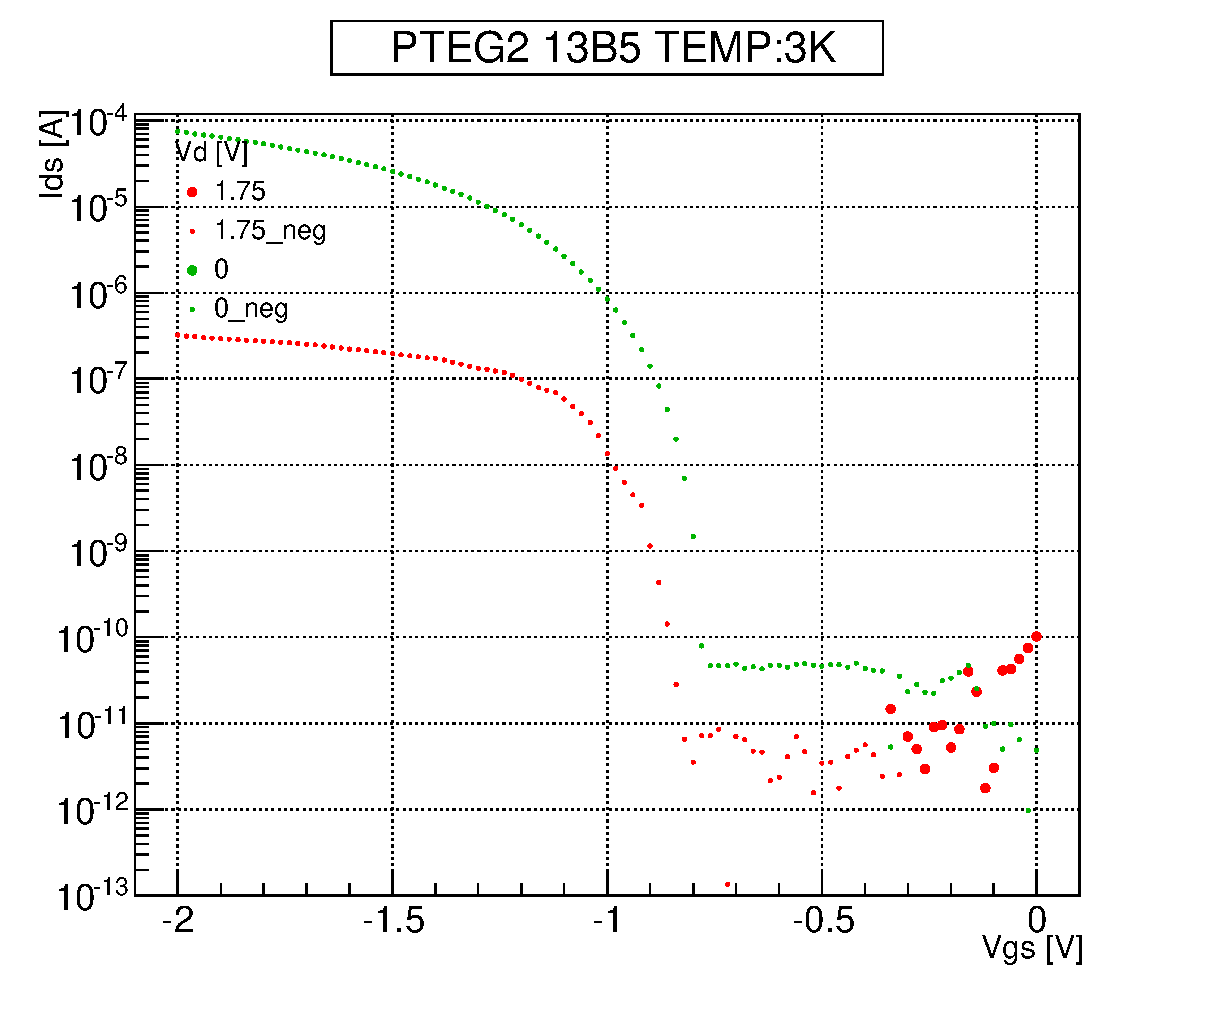
\includegraphics[width=70mm]{./Chapter/Appendix/Picture/PBT/B5/PTEG2_13_B5_IdVg_3K.eps}
						\end{center}
						\caption{B5(W/L=$0.2\mathrm{\mu m}/0.5\mathrm{\mu m}$)の$I_{ds}-V_{gs}$特性(3K)}
						\label{fig:B5_IdVg_3K}
					\end{minipage}
					\begin{minipage}{0.5\hsize}
						\begin{center}
							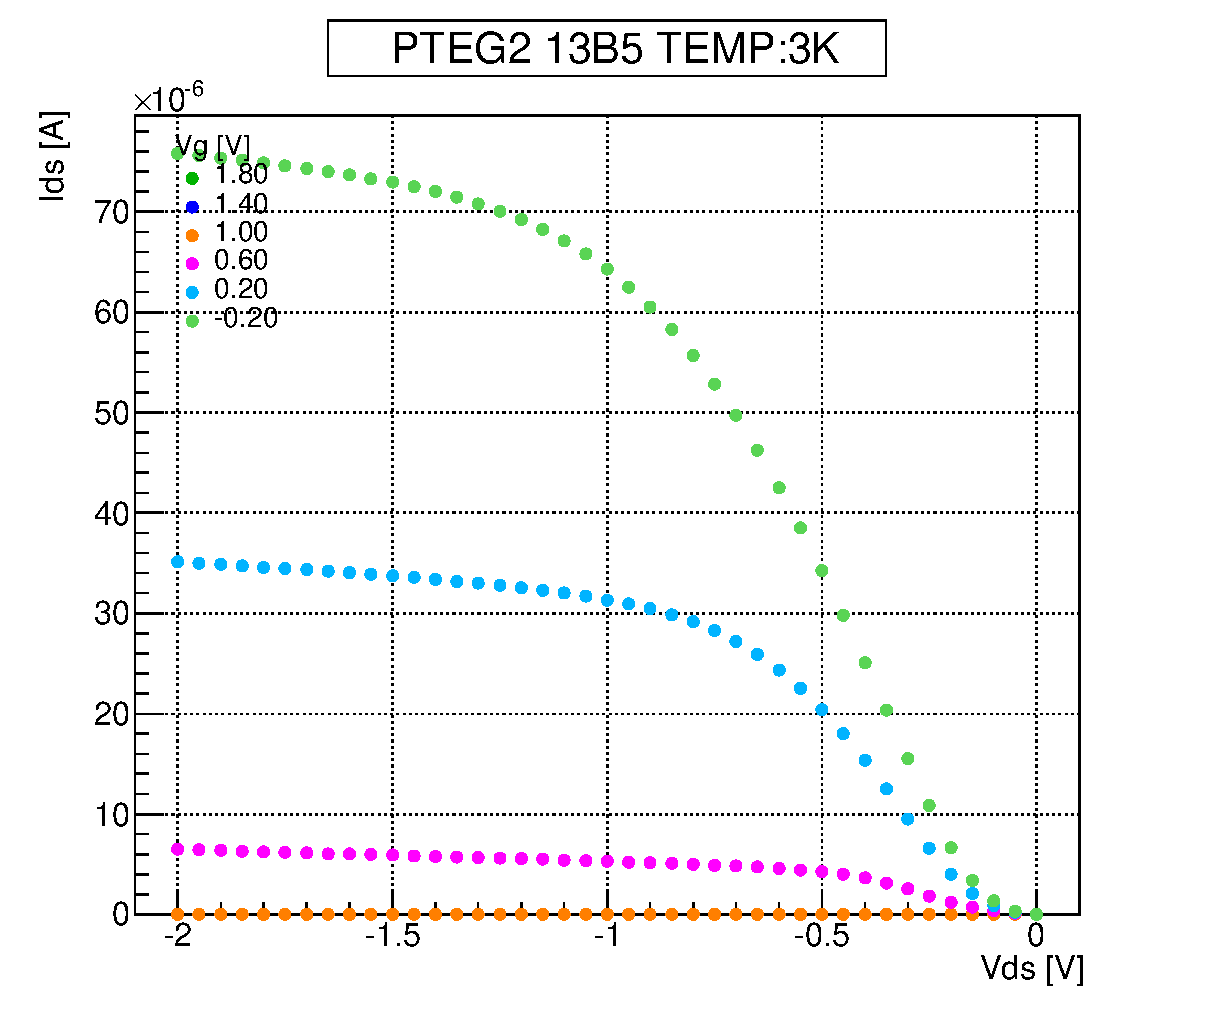
\includegraphics[width=70mm]{./Chapter/Appendix/Picture/PBT/B5/PTEG2_13_B5_IdVd_3K.eps}
						\end{center}
						\caption{B5(W/L=$0.2\mathrm{\mu m}/0.5\mathrm{\mu m}$)の$I_{ds}-V_{ds}$特性(3K)}
						\label{fig:B5_IdVd_3K}
					\end{minipage}
				\end{figure}
				%=====B6=====%
				\begin{figure}[htbp]
					\begin{minipage}{0.5\hsize}
						\begin{center}
							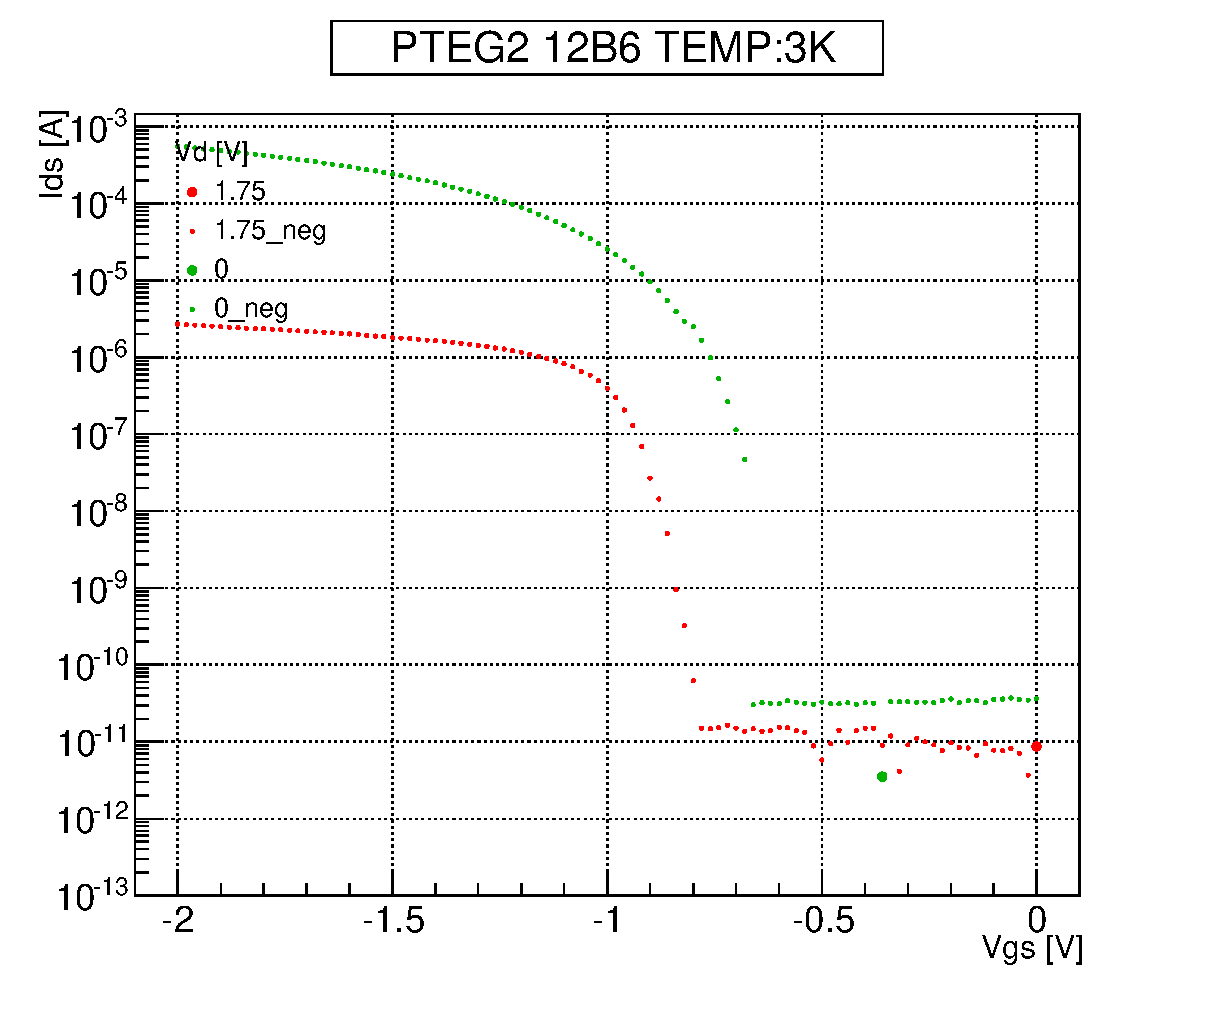
\includegraphics[width=70mm]{./Chapter/Appendix/Picture/PBT/B6/PTEG2_12_B6_IdVg_3K.eps}
						\end{center}
						\caption{B6(W/L=$0.2\mathrm{\mu m}/5\mathrm{\mu m}$)の$I_{ds}-V_{gs}$特性(3K)}
						\label{fig:B6_IdVg_3K}
					\end{minipage}
					\begin{minipage}{0.5\hsize}
						\begin{center}
							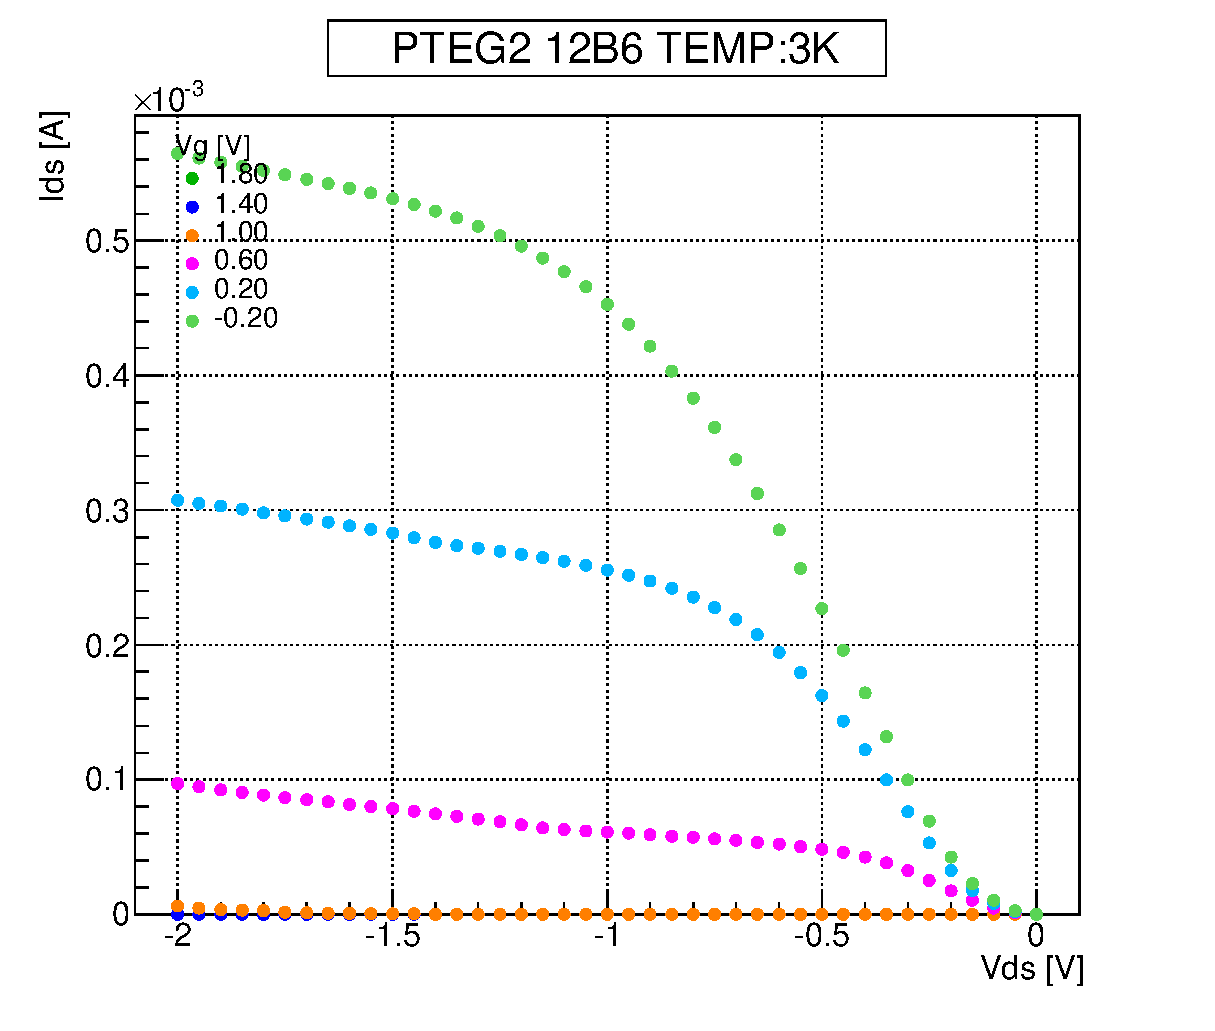
\includegraphics[width=70mm]{./Chapter/Appendix/Picture/PBT/B6/PTEG2_12_B6_IdVd_3K.eps}
						\end{center}
						\caption{B6(W/L=$0.2\mathrm{\mu m}/5\mathrm{\mu m}$)の$I_{ds}-V_{ds}$特性(3K)}
						\label{fig:B6_IdVd_3K}
					\end{minipage}
				\end{figure}
				%=====B7=====%
				\begin{figure}[htbp]
					\begin{minipage}{0.5\hsize}
						\begin{center}
							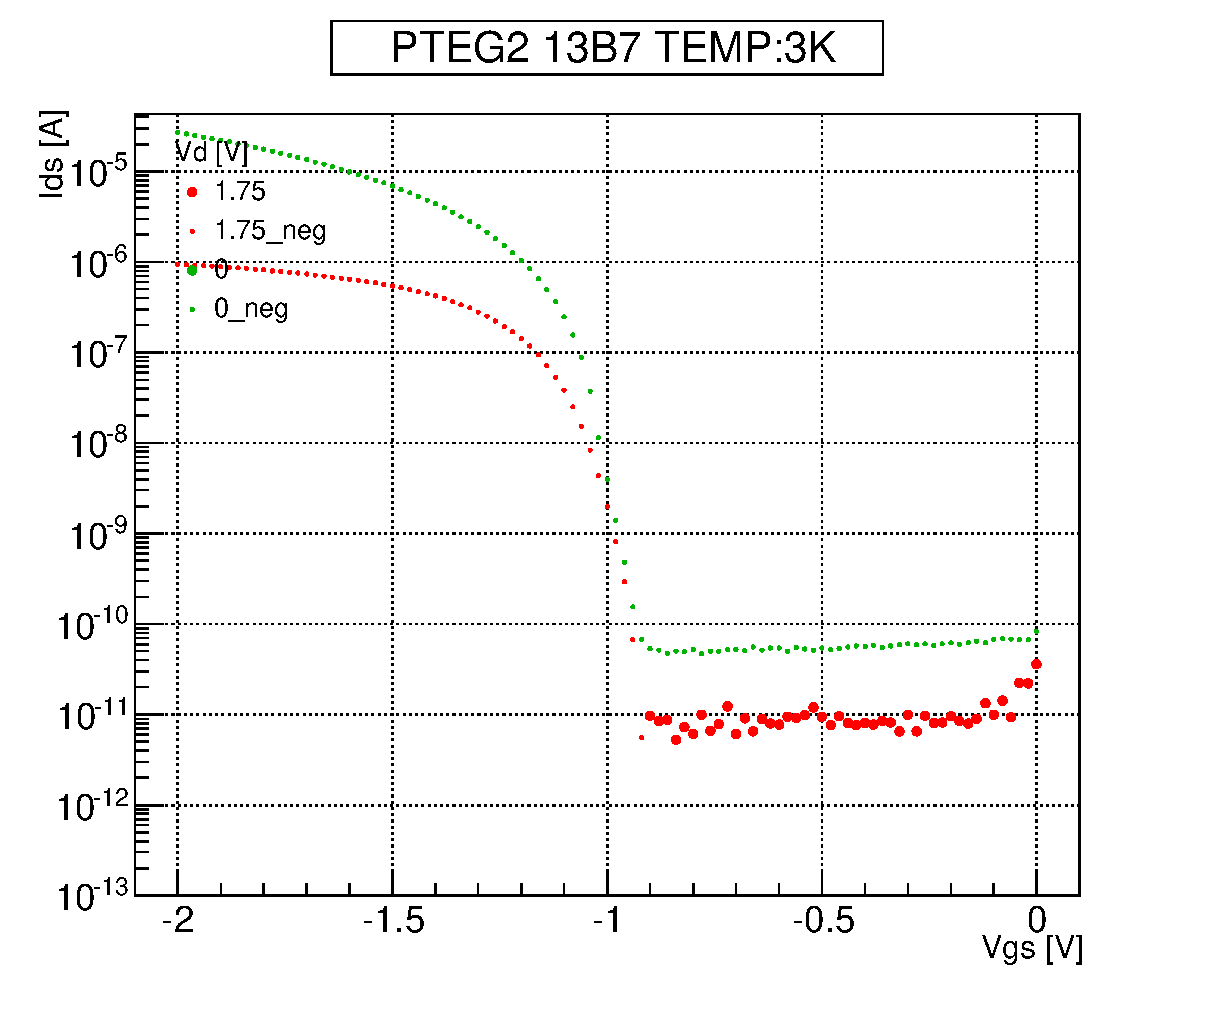
\includegraphics[width=70mm]{./Chapter/Appendix/Picture/PBT/B7/PTEG2_13_B7_IdVg_3K.eps}
						\end{center}
						\caption{B7(W/L=$10\mathrm{\mu m}/5\mathrm{\mu m}$)の$I_{ds}-V_{gs}$特性(3K)}
						\label{fig:B7_IdVg_3K}
					\end{minipage}
					\begin{minipage}{0.5\hsize}
						\begin{center}
							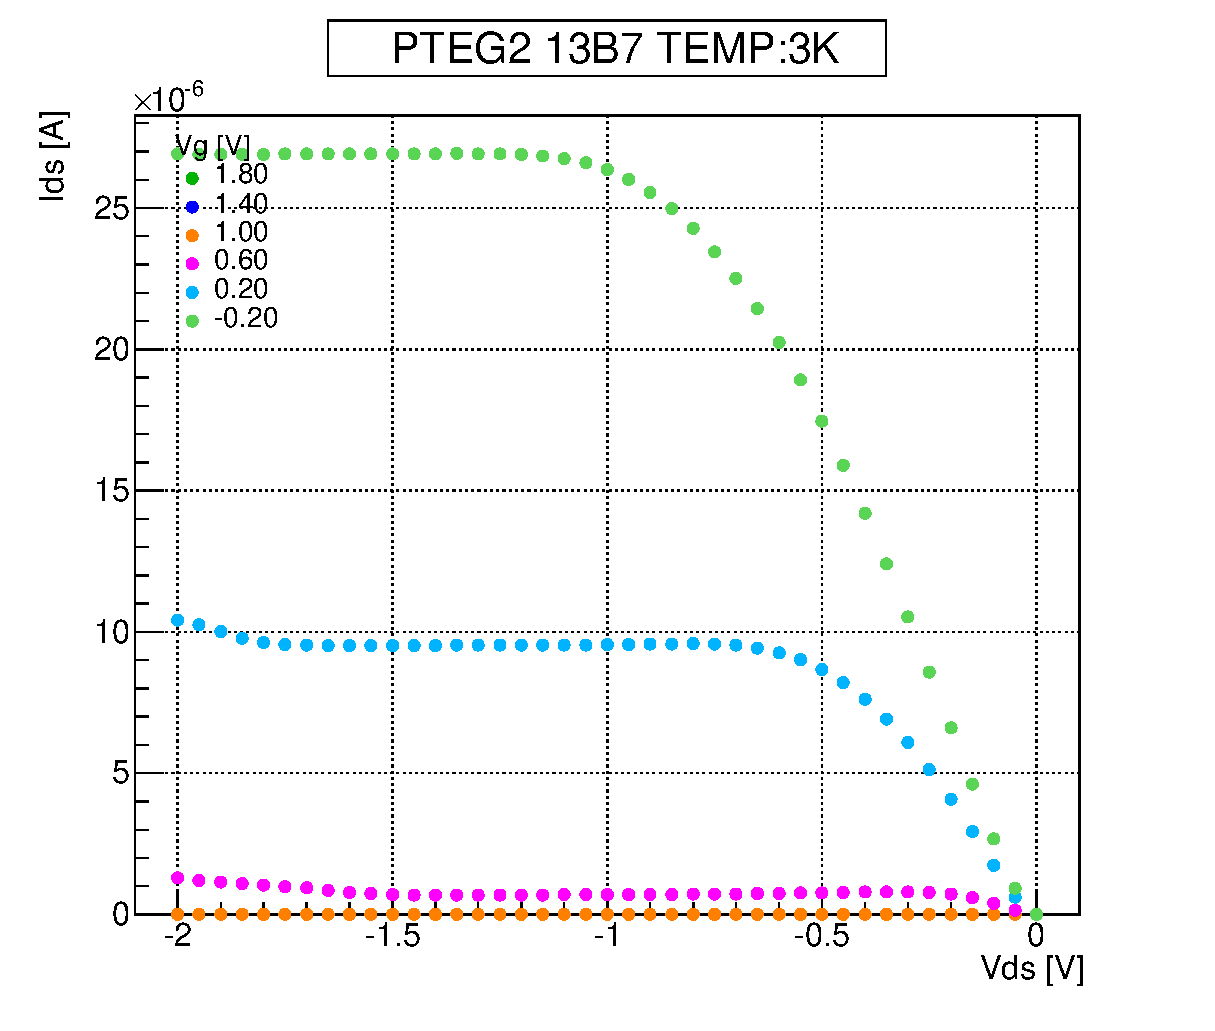
\includegraphics[width=70mm]{./Chapter/Appendix/Picture/PBT/B7/PTEG2_13_B7_IdVd_3K.eps}
						\end{center}
						\caption{B7(W/L=$10\mathrm{\mu m}/5\mathrm{\mu m}$)の$I_{ds}-V_{ds}$特性(3K)}
						\label{fig:B7_IdVd_3K}
					\end{minipage}
				\end{figure}
				%=====B8=====%
				\begin{figure}[htbp]
					\begin{minipage}{0.5\hsize}
						\begin{center}
							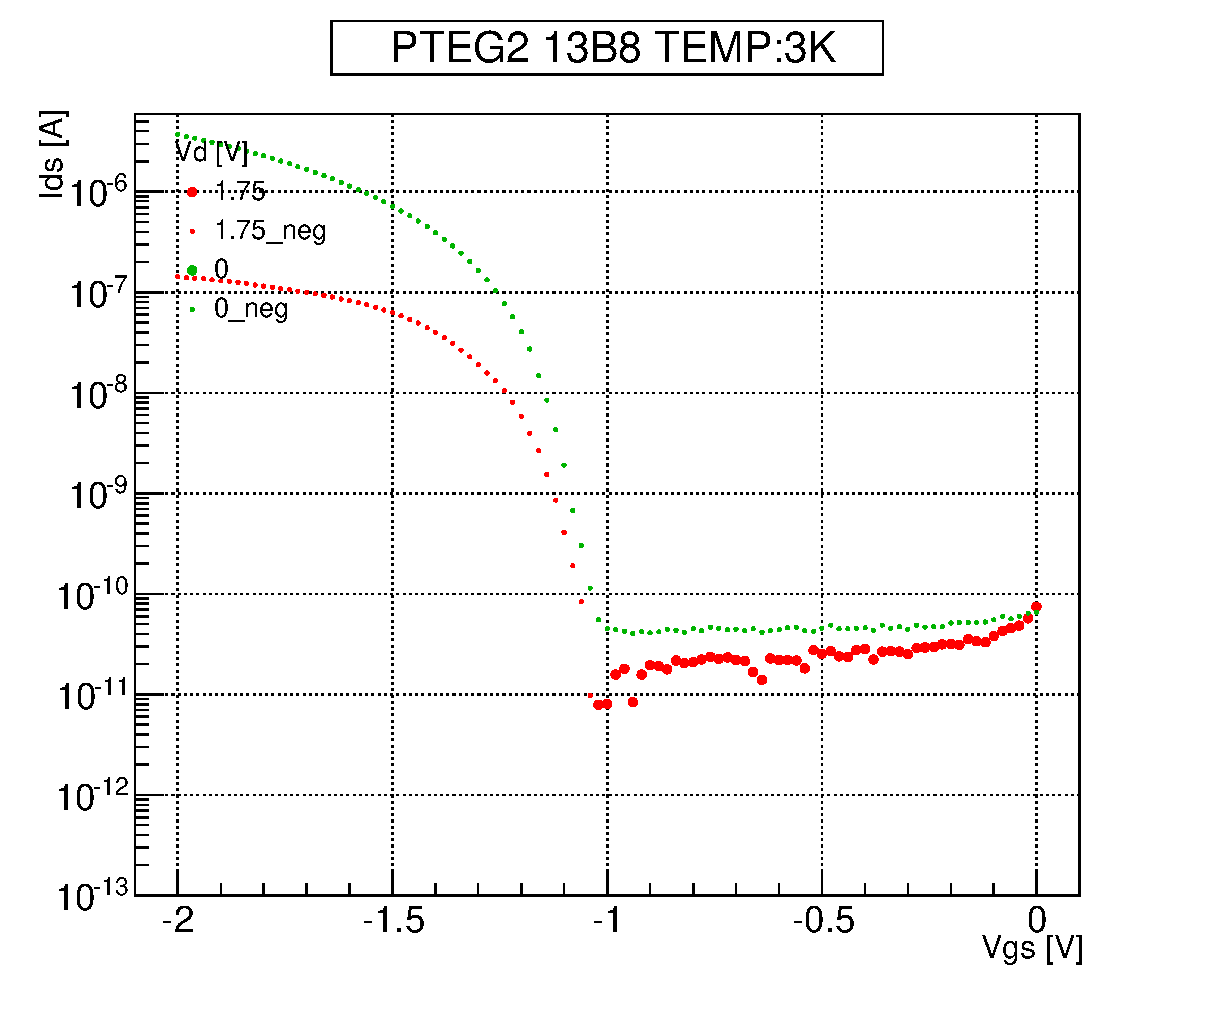
\includegraphics[width=70mm]{./Chapter/Appendix/Picture/PBT/B8/PTEG2_13_B8_IdVg_3K.eps}
						\end{center}
						\caption{B8(W/L=$10\mathrm{\mu m}/0.63\mathrm{\mu m}$)の$I_{ds}-V_{gs}$特性(3K)}
						\label{fig:B8_IdVg_3K}
					\end{minipage}
					\begin{minipage}{0.5\hsize}
						\begin{center}
							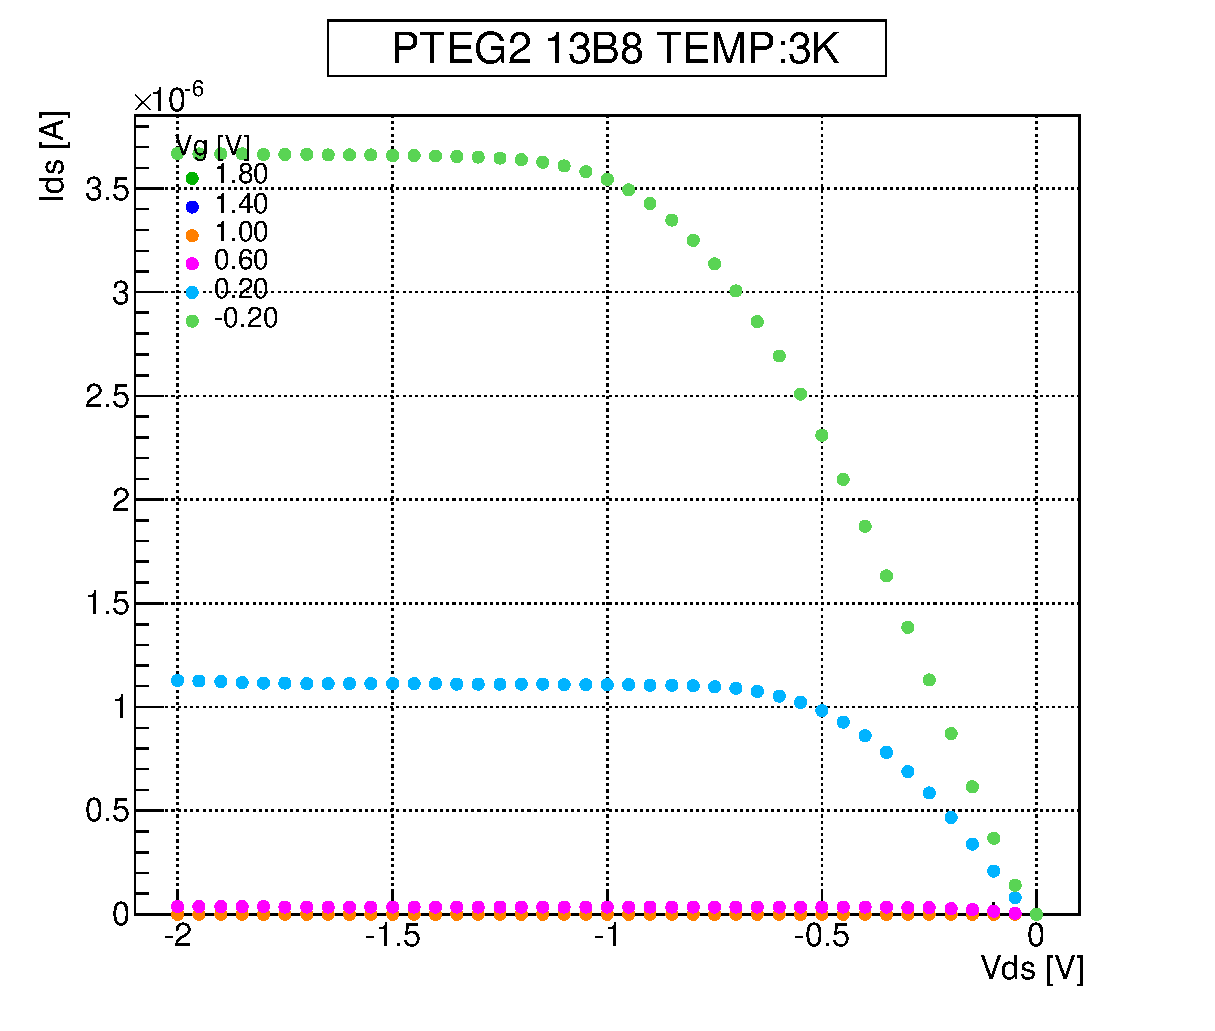
\includegraphics[width=70mm]{./Chapter/Appendix/Picture/PBT/B8/PTEG2_13_B8_IdVd_3K.eps}
						\end{center}
						\caption{B8(W/L=$10\mathrm{\mu m}/0.63\mathrm{\mu m}$)の$I_{ds}-V_{ds}$特性(3K)}
						\label{fig:B8_IdVd_3K}
					\end{minipage}
				\end{figure}
				\clearpage
		%=====ここからST type=====%
		\section{NMOS-ST2(常温環境)}
				%=====NS1=====%
				\begin{figure}[htbp]
					\begin{minipage}{0.5\hsize}
						\begin{center}
							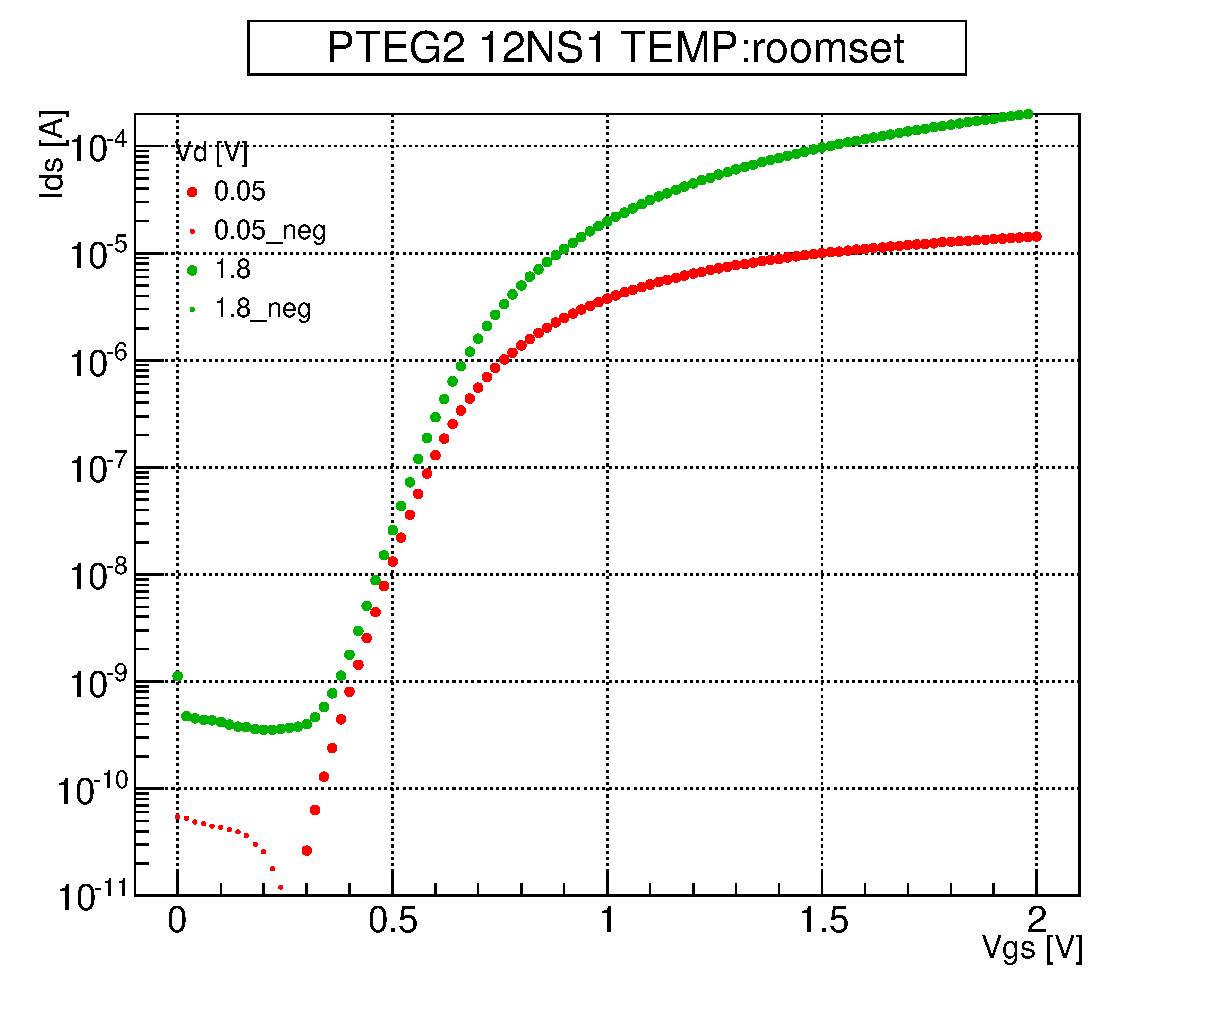
\includegraphics[width=70mm]{./Chapter/Appendix/Picture/NST/NS1/PTEG2_12_NS1_IdVg_roomset.eps}
						\end{center}
						\caption{NS1(W/L=$0.4\mathrm{\mu m}/1\mathrm{\mu m}$)の$I_{ds}-V_{gs}$特性(常温)}
						\label{fig:NS1_IdVg_room}
					\end{minipage}
					\begin{minipage}{0.5\hsize}
						\begin{center}
							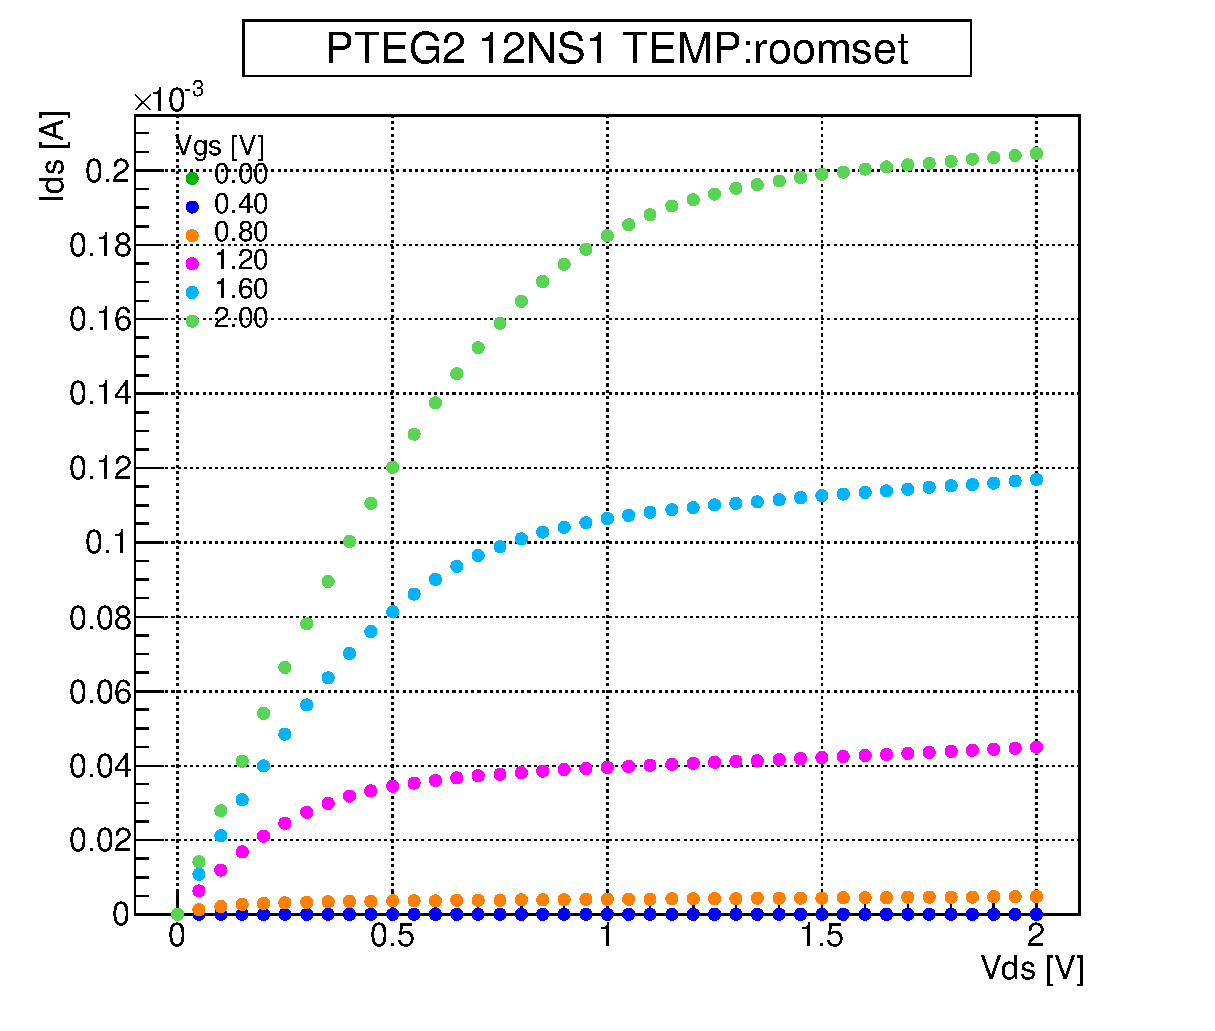
\includegraphics[width=70mm]{./Chapter/Appendix/Picture/NST/NS1/PTEG2_12_NS1_IdVd_roomset.eps}
						\end{center}
						\caption{NS1(W/L=$0.4\mathrm{\mu m}/1\mathrm{\mu m}$)の$I_{ds}-V_{ds}$特性(常温)}
						\label{fig:NS1_IdVd_room}
					\end{minipage}
				\end{figure}
				%=====NS2=====%
				\begin{figure}[htbp]
					\begin{minipage}{0.5\hsize}
						\begin{center}
							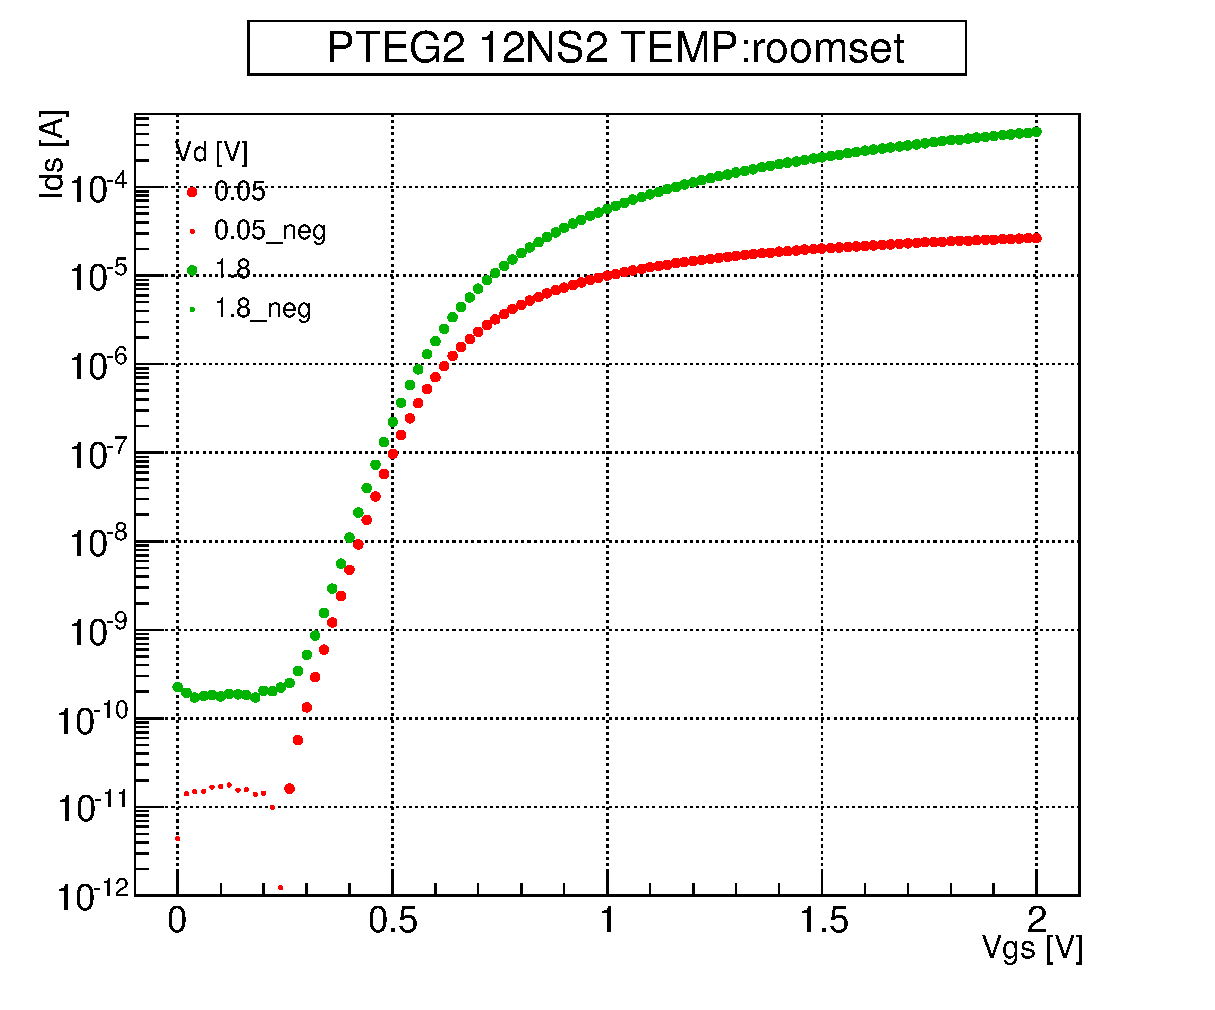
\includegraphics[width=70mm]{./Chapter/Appendix/Picture/NST/NS2/PTEG2_12_NS2_IdVg_roomset.eps}
						\end{center}
						\caption{NS2(W/L=$0.4\mathrm{\mu m}/2\mathrm{\mu m}$)の$I_{ds}-V_{gs}$特性(常温)}
						\label{fig:NS2_IdVg_room}
					\end{minipage}
					\begin{minipage}{0.5\hsize}
						\begin{center}
							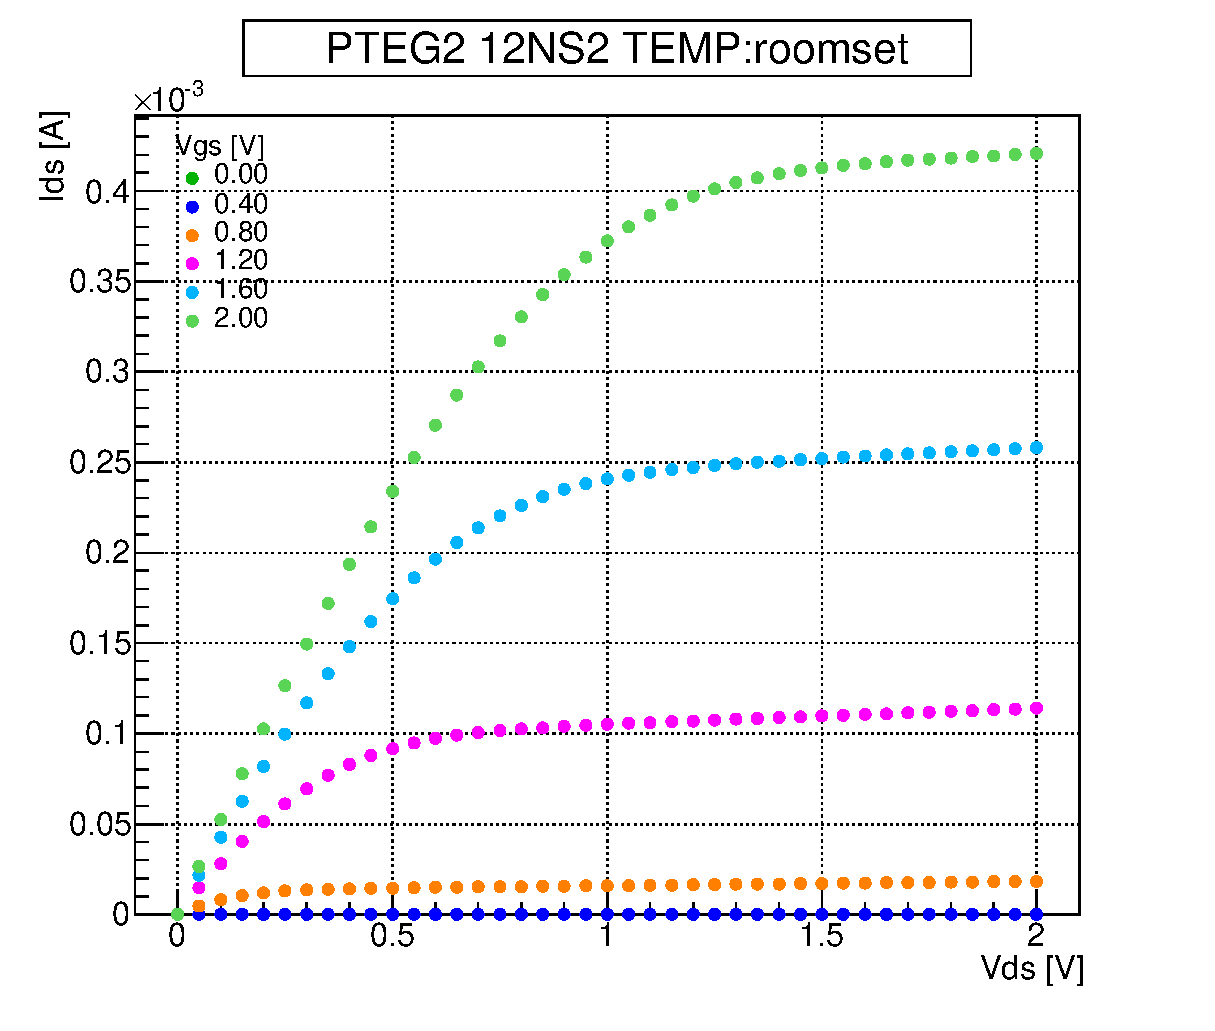
\includegraphics[width=70mm]{./Chapter/Appendix/Picture/NST/NS2/PTEG2_12_NS2_IdVd_roomset.eps}
						\end{center}
						\caption{NS2(W/L=$0.4\mathrm{\mu m}/2\mathrm{\mu m}$)の$I_{ds}-V_{ds}$特性(常温)}
						\label{fig:NS2_IdVd_room}
					\end{minipage}
				\end{figure}
				%=====NS3=====%
				\begin{figure}[htbp]
					\begin{minipage}{0.5\hsize}
						\begin{center}
							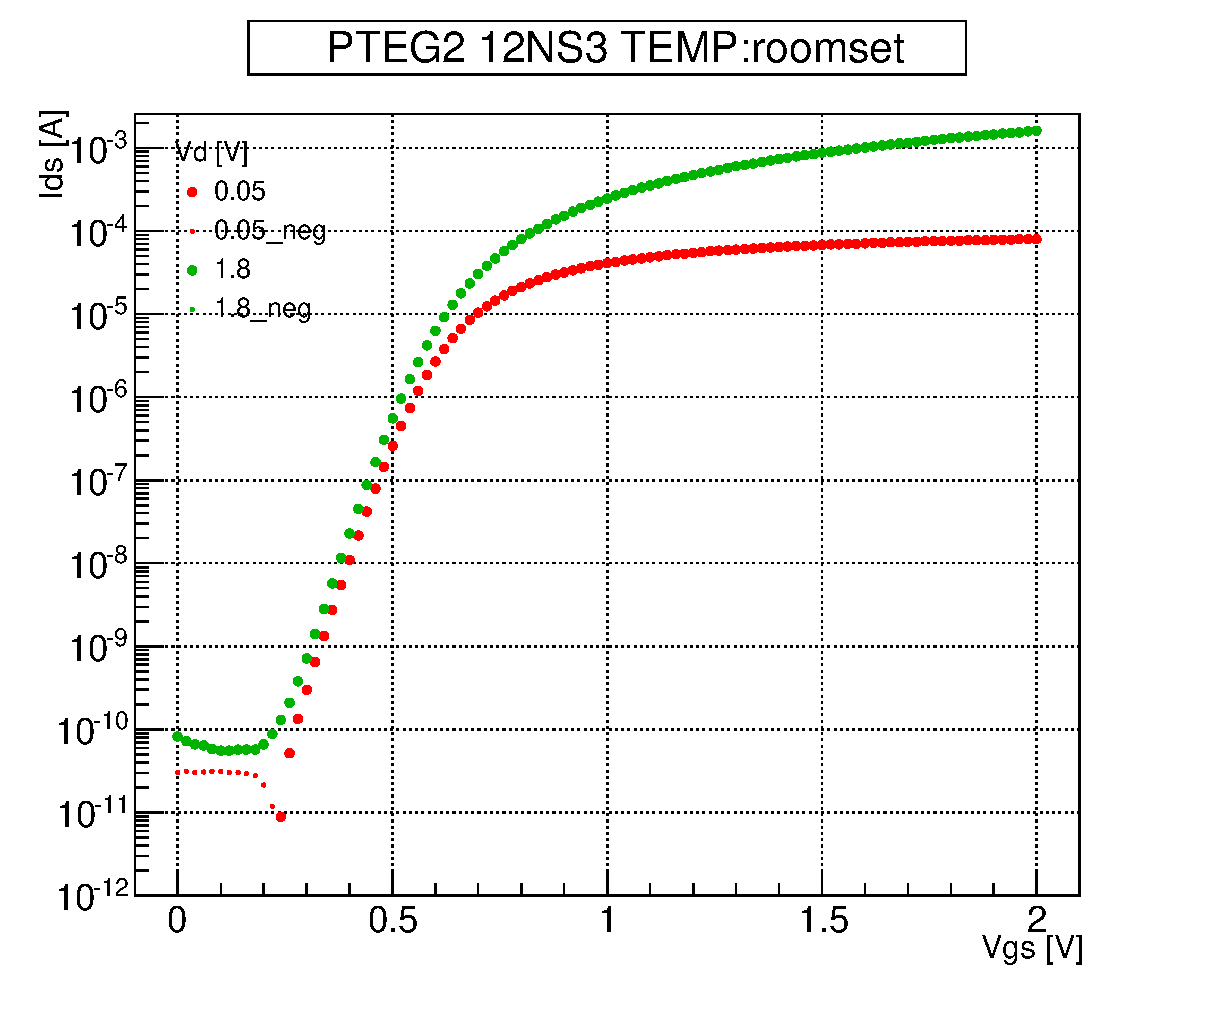
\includegraphics[width=70mm]{./Chapter/Appendix/Picture/NST/NS3/PTEG2_12_NS3_IdVg_roomset.eps}
						\end{center}
						\caption{NS3(W/L=$0.4\mathrm{\mu m}/10\mathrm{\mu m}$)の$I_{ds}-V_{gs}$特性(常温)}
						\label{fig:NS3_IdVg_room}
					\end{minipage}
					\begin{minipage}{0.5\hsize}
						\begin{center}
							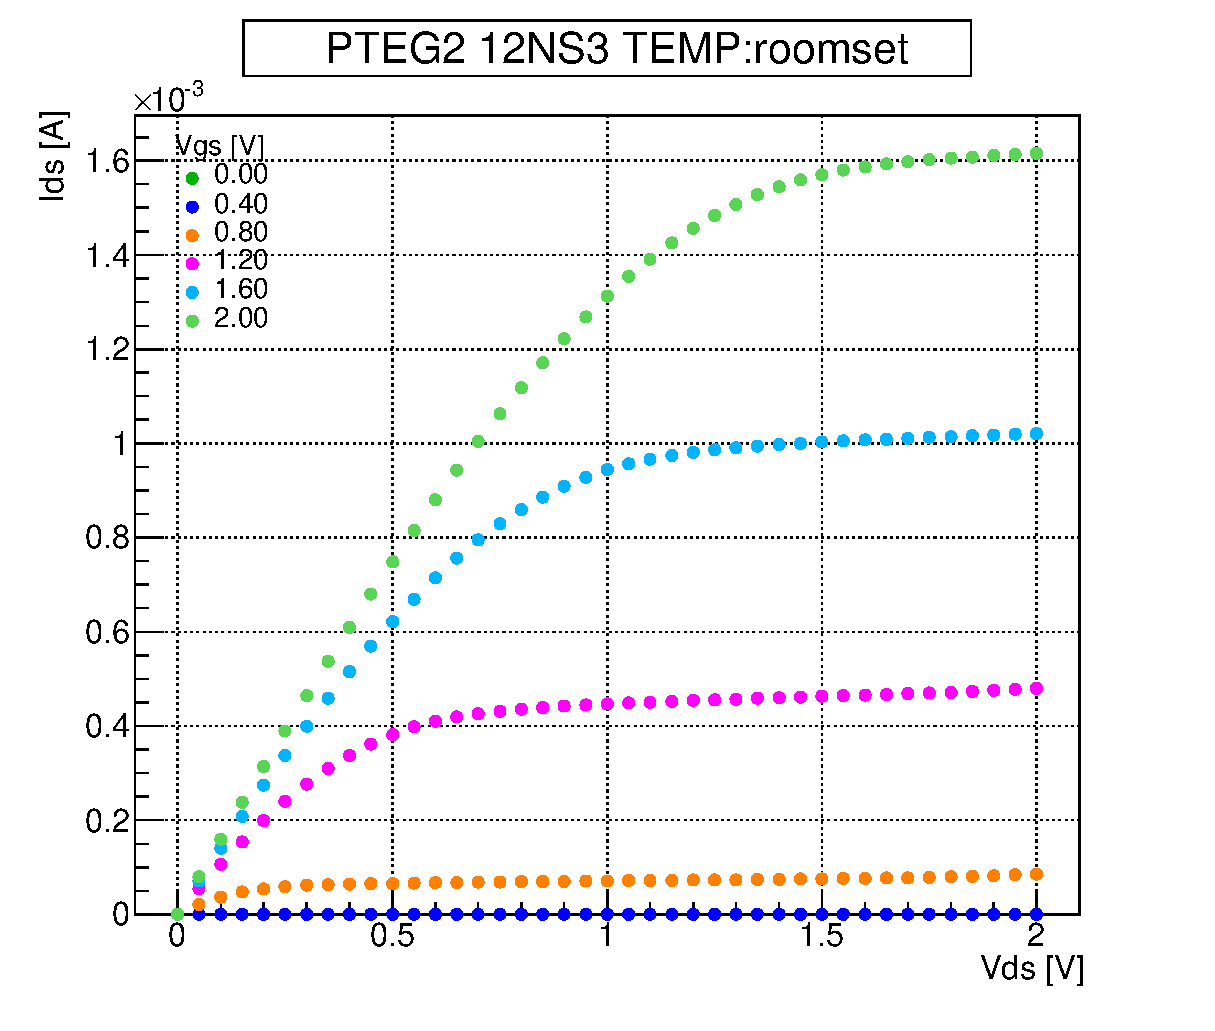
\includegraphics[width=70mm]{./Chapter/Appendix/Picture/NST/NS3/PTEG2_12_NS3_IdVd_roomset.eps}
						\end{center}
						\caption{NS3(W/L=$0.4\mathrm{\mu m}/10\mathrm{\mu m}$)の$I_{ds}-V_{ds}$特性(常温)}
						\label{fig:NS3_IdVd_room}
					\end{minipage}
				\end{figure}
				%=====NS4=====%
				\begin{figure}[htbp]
					\begin{minipage}{0.5\hsize}
						\begin{center}
							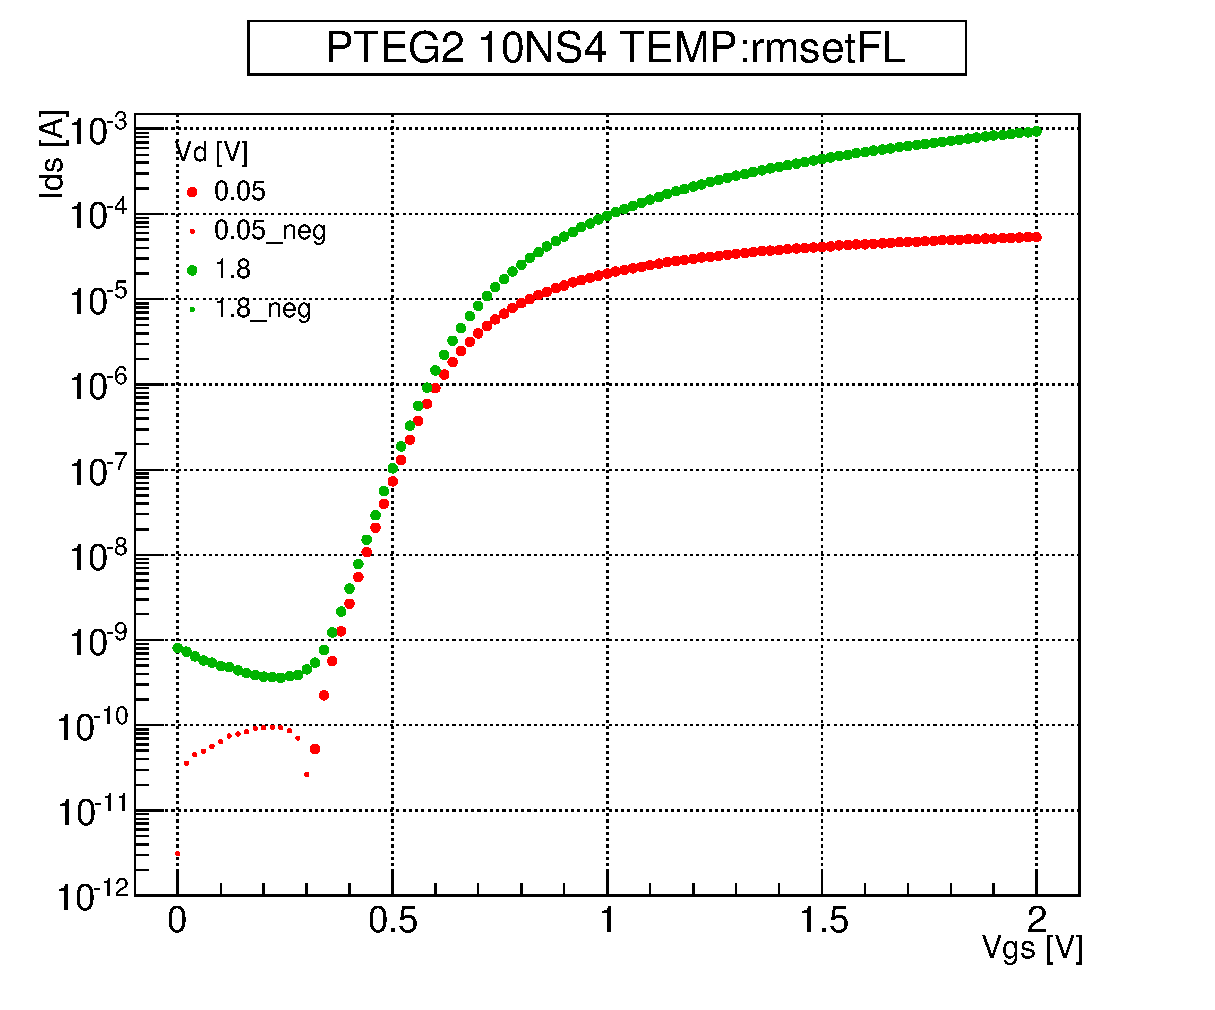
\includegraphics[width=70mm]{./Chapter/Appendix/Picture/NST/NS4/PTEG2_10_NS4_IdVg_rmsetFL.eps}
						\end{center}
						\caption{NS4(W/L=$1\mathrm{\mu m}/10\mathrm{\mu m}$)の$I_{ds}-V_{gs}$特性(常温)}
						\label{fig:NS4_IdVg_room}
					\end{minipage}
					\begin{minipage}{0.5\hsize}
						\begin{center}
							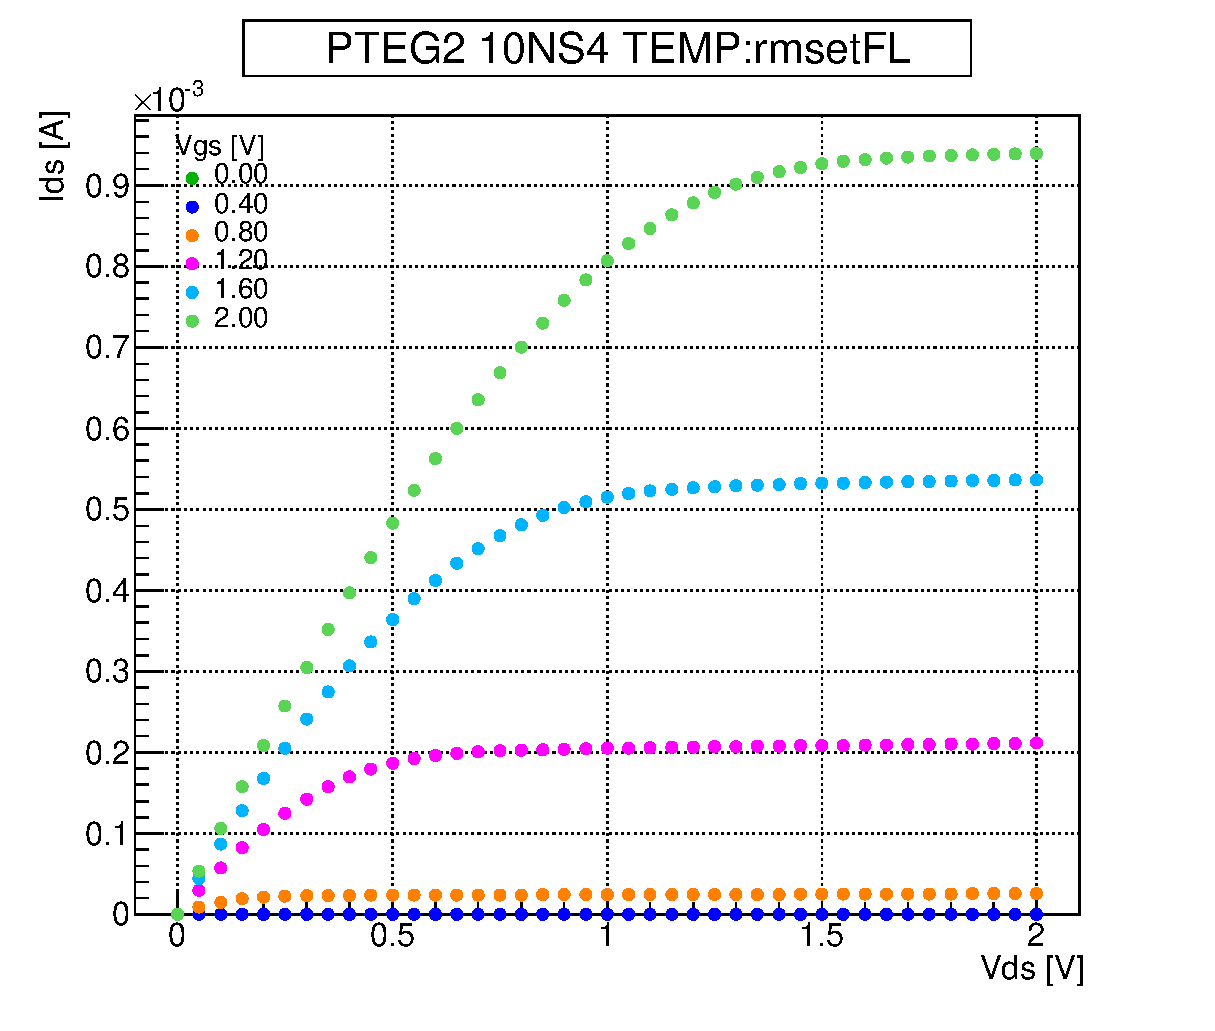
\includegraphics[width=70mm]{./Chapter/Appendix/Picture/NST/NS4/PTEG2_10_NS4_IdVd_rmsetFL.eps}
						\end{center}
						\caption{NS4(W/L=$0.4\mathrm{\mu m}/10\mathrm{\mu m}$)の$I_{ds}-V_{ds}$特性(常温)}
						\label{fig:NS4_IdVd_room}
					\end{minipage}
				\end{figure}
				%=====NS5=====%
				\begin{figure}[htbp]
					\begin{minipage}{0.5\hsize}
						\begin{center}
							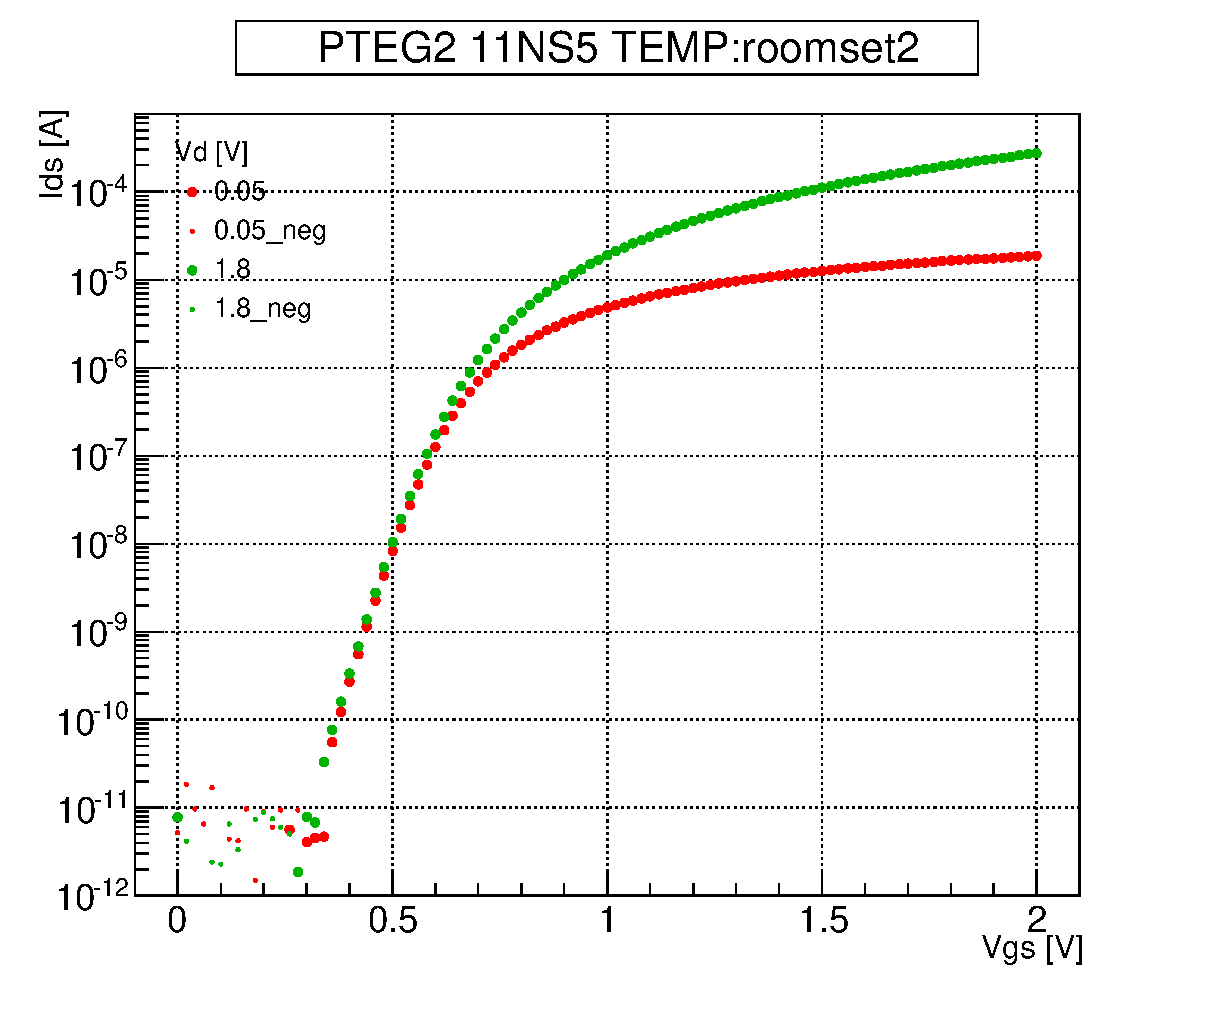
\includegraphics[width=70mm]{./Chapter/Appendix/Picture/NST/NS5/PTEG2_11_NS5_IdVg_roomset2.eps}
						\end{center}
						\caption{NS5(W/L=$5\mathrm{\mu m}/10\mathrm{\mu m}$)の$I_{ds}-V_{gs}$特性(常温)}
						\label{fig:NS5_IdVg_room}
					\end{minipage}
					\begin{minipage}{0.5\hsize}
						\begin{center}
							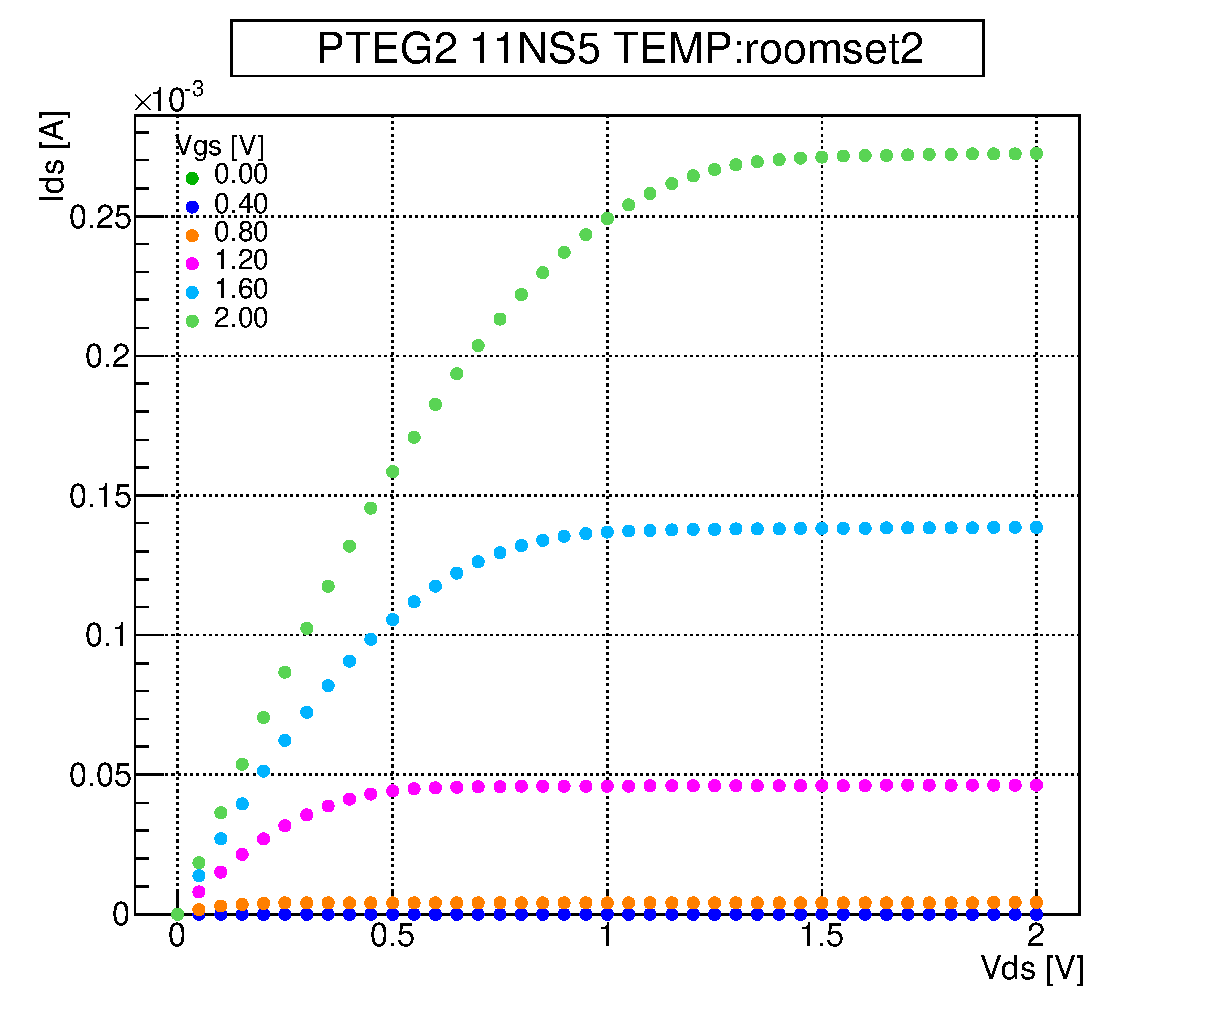
\includegraphics[width=70mm]{./Chapter/Appendix/Picture/NST/NS5/PTEG2_11_NS5_IdVd_roomset2.eps}
						\end{center}
						\caption{NS5(W/L=$5\mathrm{\mu m}/10\mathrm{\mu m}$)の$I_{ds}-V_{ds}$特性(常温)}
						\label{fig:NS5_IdVd_room}
					\end{minipage}
				\end{figure}
				%=====NS6=====%
				\begin{figure}[htbp]
					\begin{minipage}{0.5\hsize}
						\begin{center}
							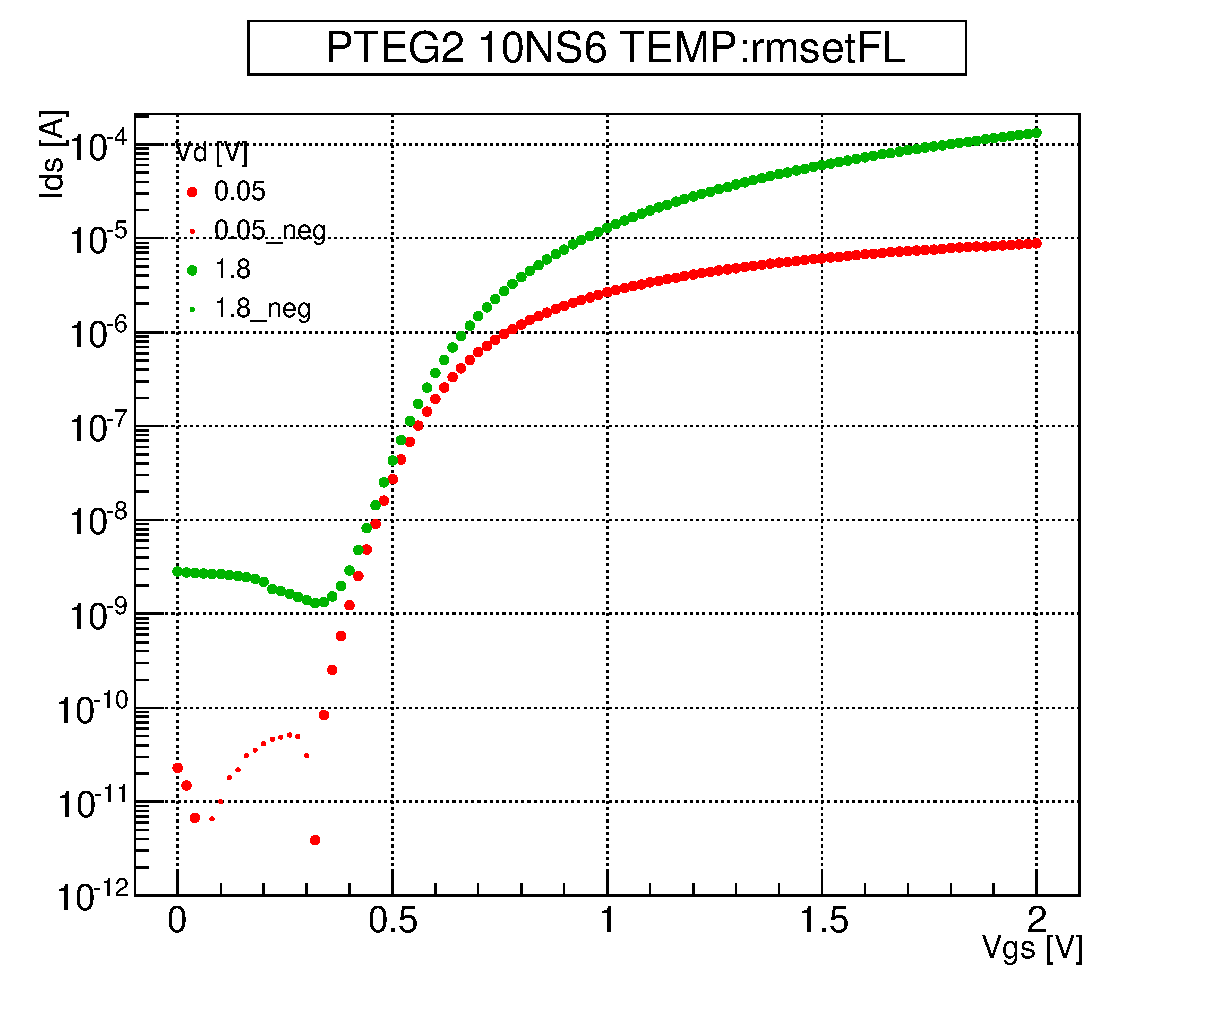
\includegraphics[width=70mm]{./Chapter/Appendix/Picture/NST/NS6/PTEG2_10_NS6_IdVg_rmsetFL.eps}
						\end{center}
						\caption{NS6(W/L=$1\mathrm{\mu m}/1\mathrm{\mu m}$)の$I_{ds}-V_{gs}$特性(常温)}
						\label{fig:NS6_IdVg_room}
					\end{minipage}
					\begin{minipage}{0.5\hsize}
						\begin{center}
							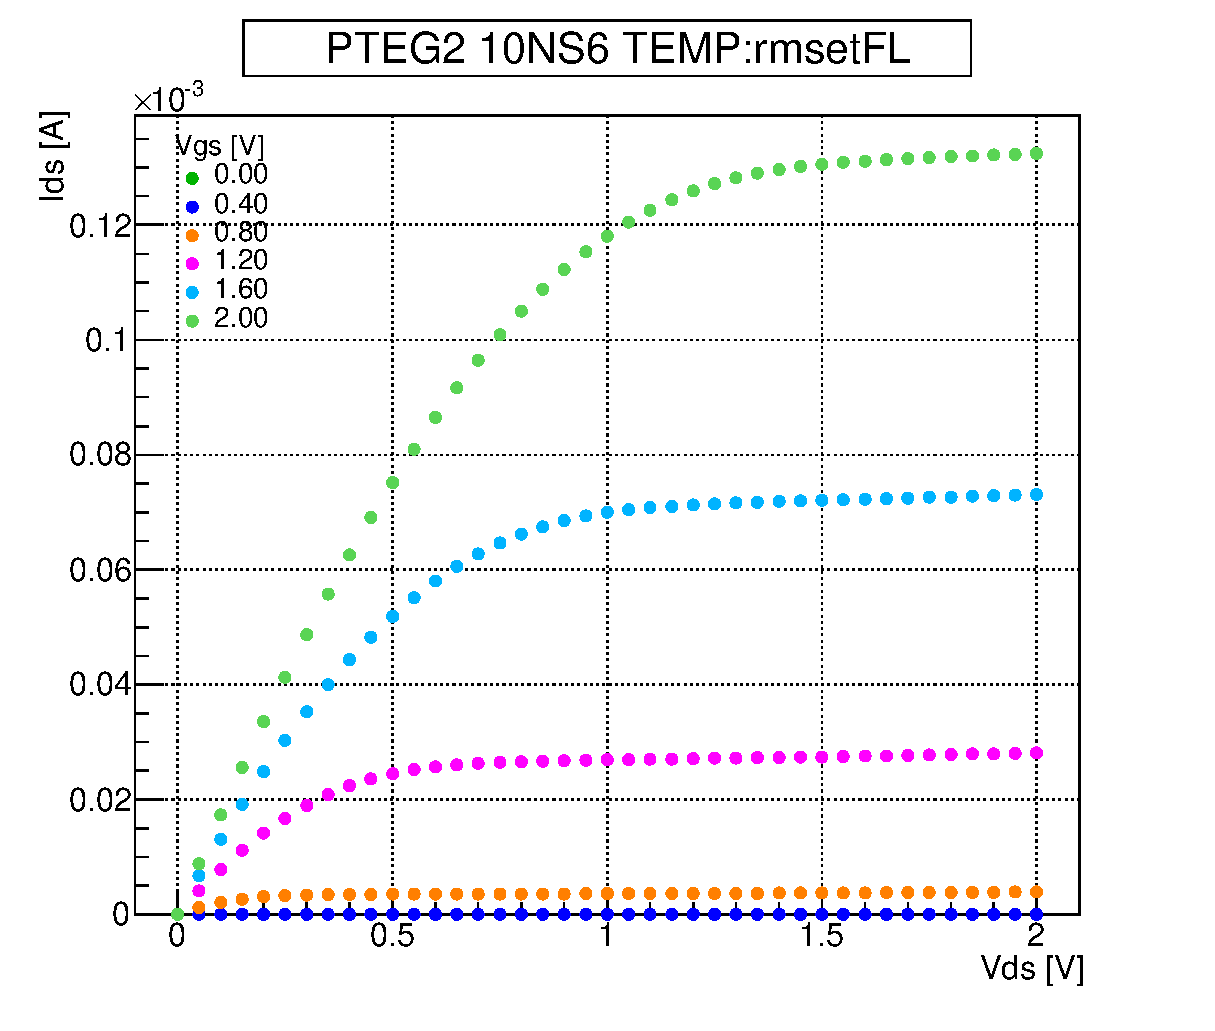
\includegraphics[width=70mm]{./Chapter/Appendix/Picture/NST/NS6/PTEG2_10_NS6_IdVd_rmsetFL.eps}
						\end{center}
						\caption{NS6(W/L=$1\mathrm{\mu m}/1\mathrm{\mu m}$)の$I_{ds}-V_{ds}$特性(常温)}
						\label{fig:NS6_IdVd_room}
					\end{minipage}
				\end{figure}
				%=====NS7=====%
				\begin{figure}[htbp]
					\begin{minipage}{0.5\hsize}
						\begin{center}
							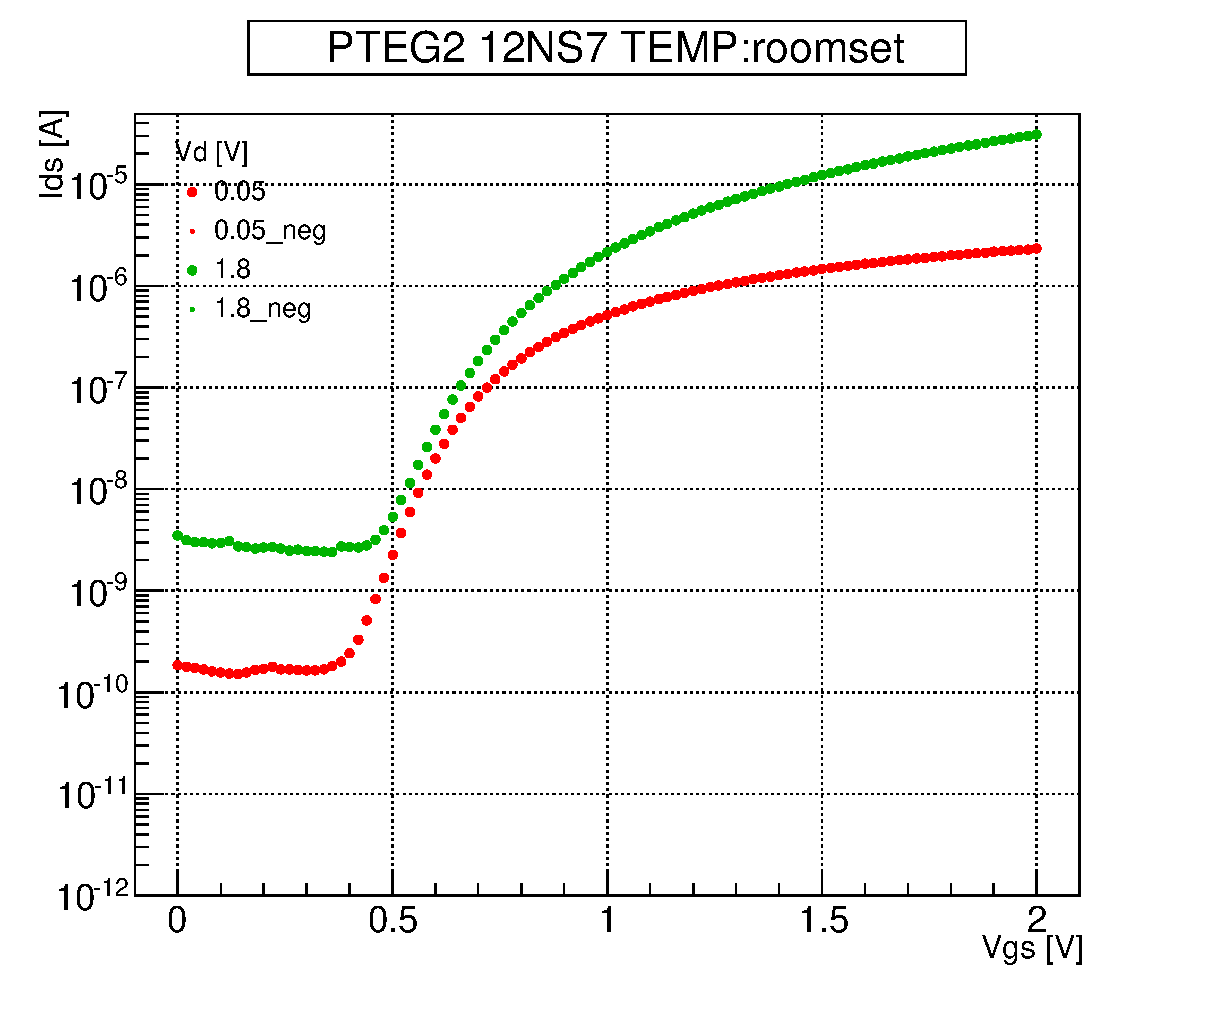
\includegraphics[width=70mm]{./Chapter/Appendix/Picture/NST/NS7/PTEG2_12_NS7_IdVg_roomset.eps}
						\end{center}
						\caption{NS7(W/L=$5\mathrm{\mu m}/1\mathrm{\mu m}$)の$I_{ds}-V_{gs}$特性(常温)}
						\label{fig:NS7_IdVg_room}
					\end{minipage}
					\begin{minipage}{0.5\hsize}
						\begin{center}
							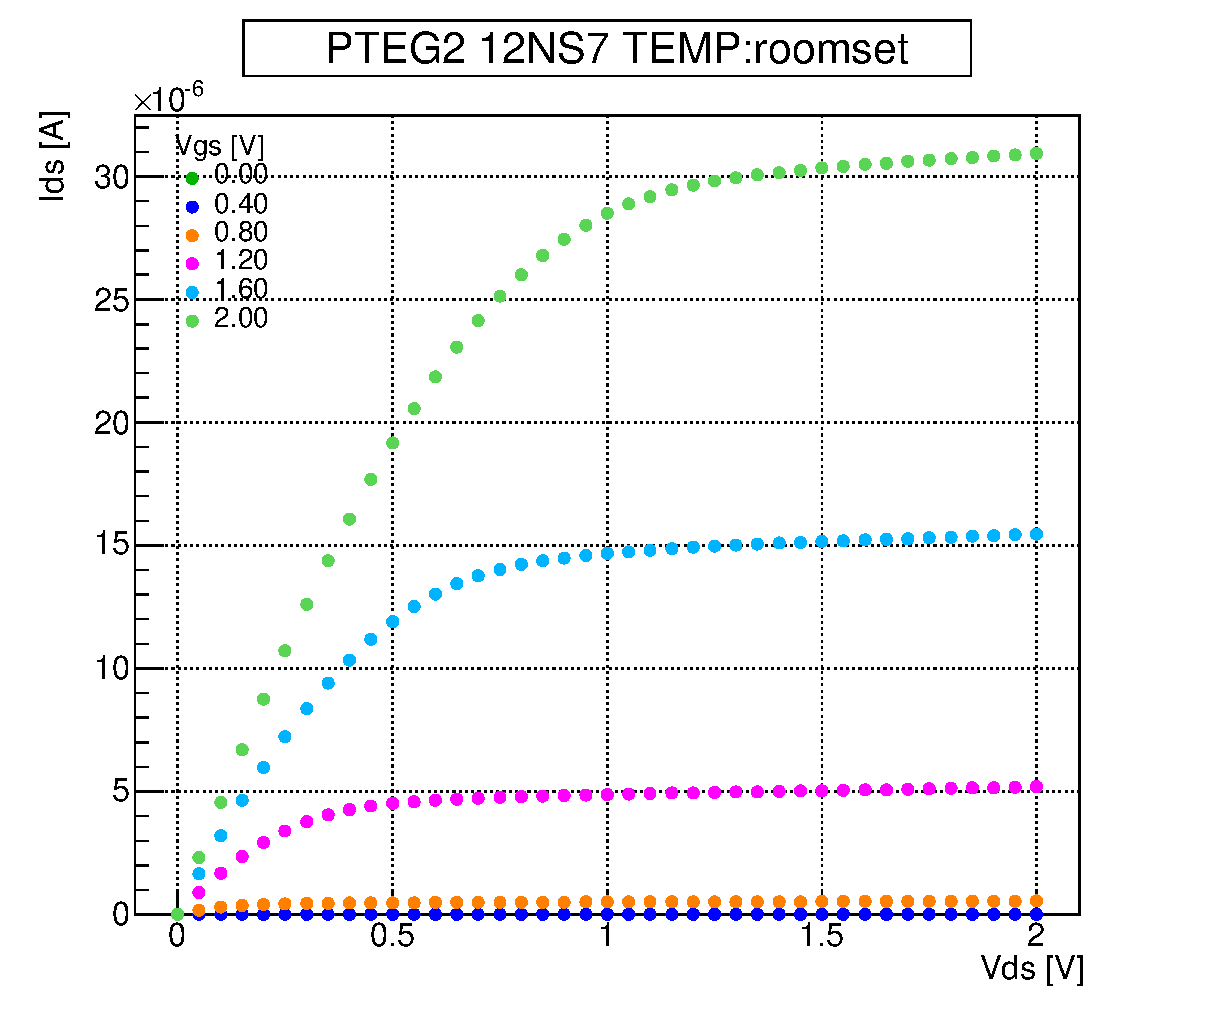
\includegraphics[width=70mm]{./Chapter/Appendix/Picture/NST/NS7/PTEG2_12_NS7_IdVd_roomset.eps}
						\end{center}
						\caption{NS7(W/L=$5\mathrm{\mu m}/1\mathrm{\mu m}$)の$I_{ds}-V_{ds}$特性(常温)}
						\label{fig:NS7_IdVd_room}
					\end{minipage}
				\end{figure}
				%=====NS8=====%
				\begin{figure}[htbp]
					\begin{minipage}{0.5\hsize}
						\begin{center}
							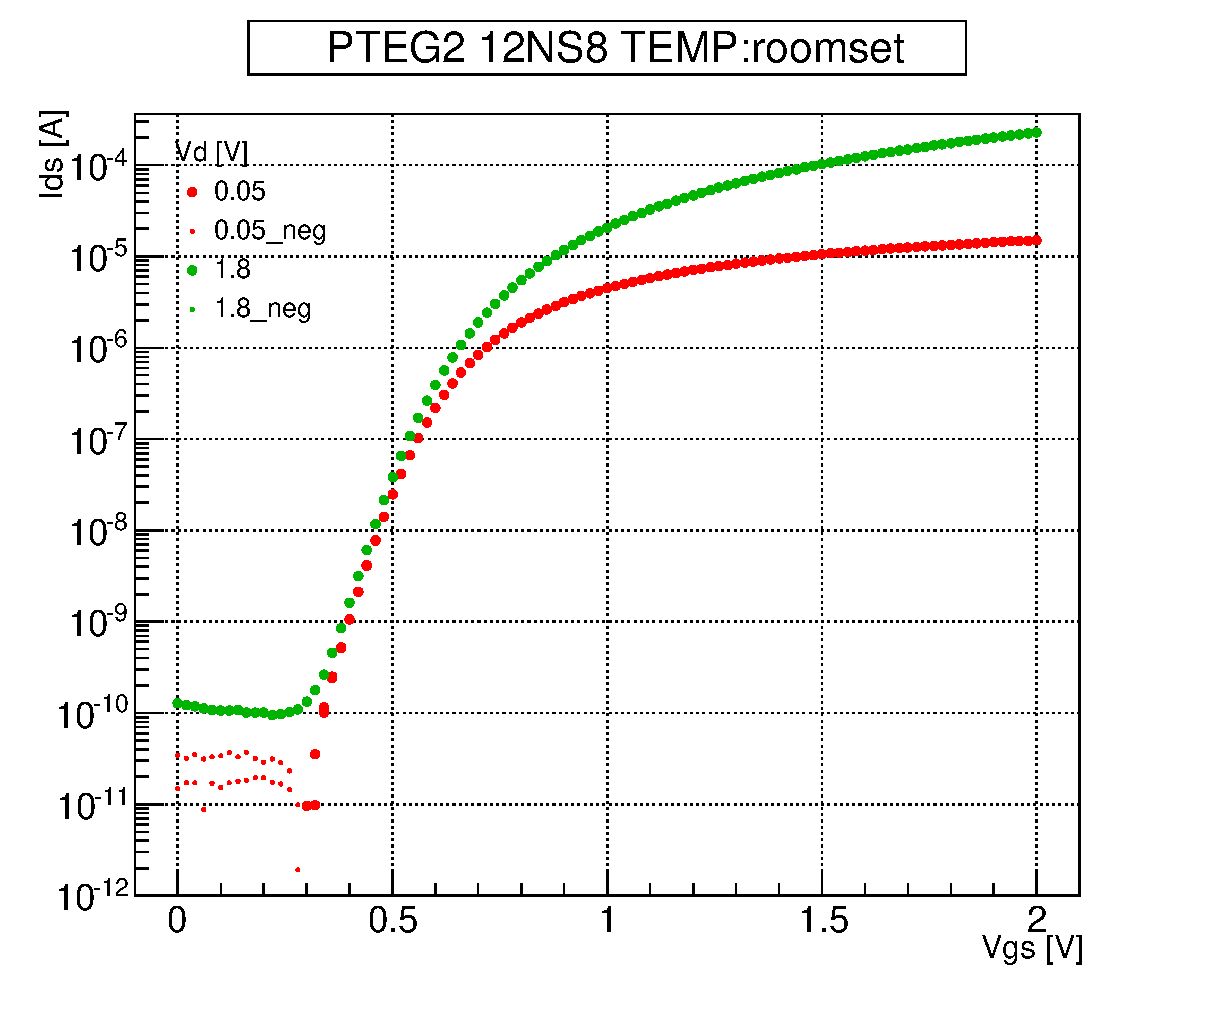
\includegraphics[width=70mm]{./Chapter/Appendix/Picture/NST/NS8/PTEG2_12_NS8_IdVg_roomset.eps}
						\end{center}
						\caption{NS8(W/L=$1\mathrm{\mu m}/2\mathrm{\mu m}$)の$I_{ds}-V_{gs}$特性(常温)}
						\label{fig:NS8_IdVg_room}
					\end{minipage}
					\begin{minipage}{0.5\hsize}
						\begin{center}
							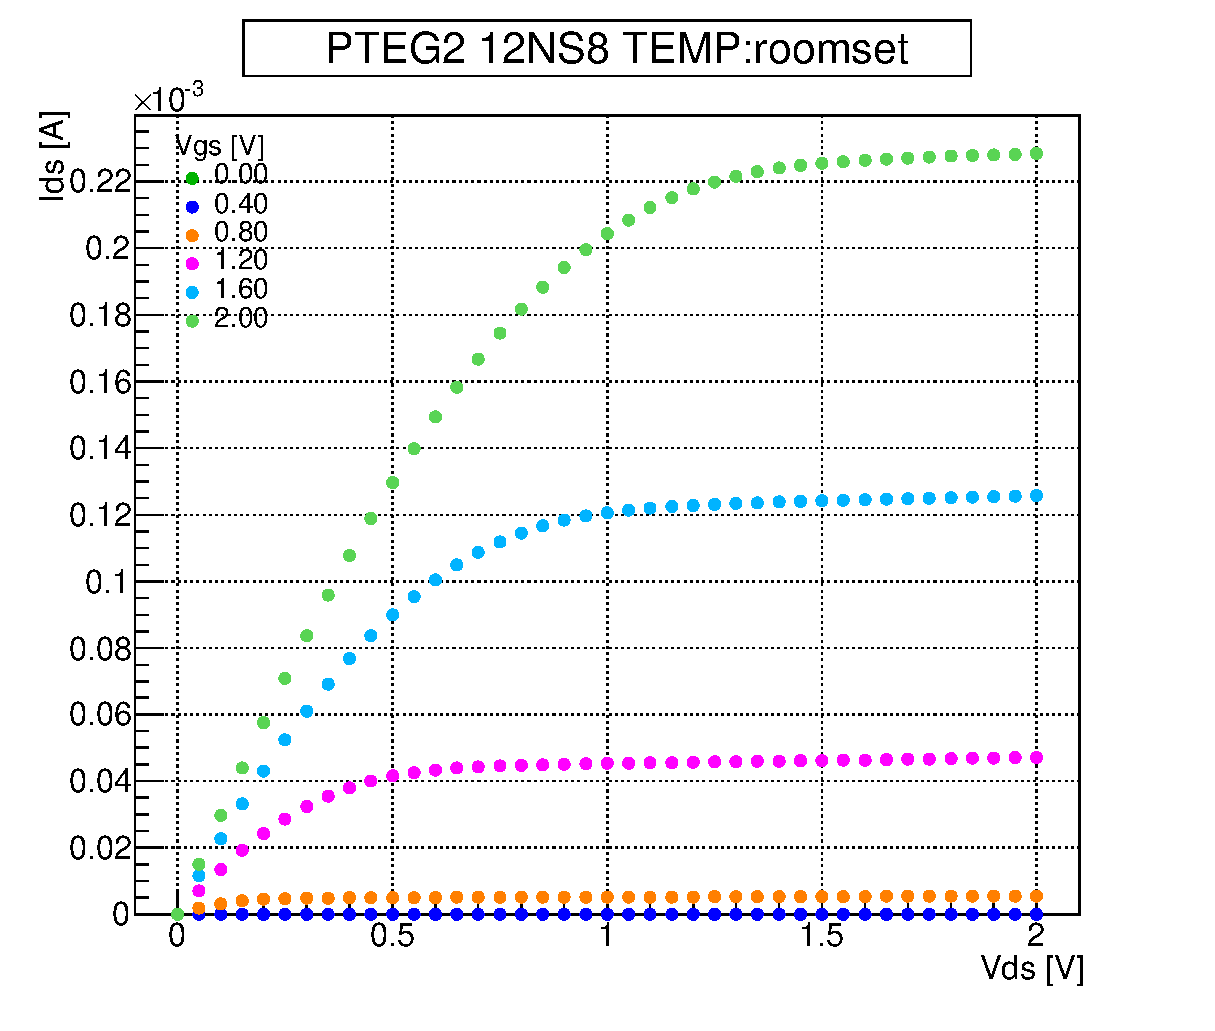
\includegraphics[width=70mm]{./Chapter/Appendix/Picture/NST/NS8/PTEG2_12_NS8_IdVd_roomset.eps}
						\end{center}
						\caption{NS8(W/L=$1\mathrm{\mu m}/2\mathrm{\mu m}$)の$I_{ds}-V_{ds}$特性(常温)}
						\label{fig:NS8_IdVd_room}
					\end{minipage}
				\end{figure}
				\clearpage
				
		\section{NMOS-ST2(3K環境)}
				%=====NS1=====%
				\begin{figure}[htbp]
					\begin{minipage}{0.5\hsize}
						\begin{center}
							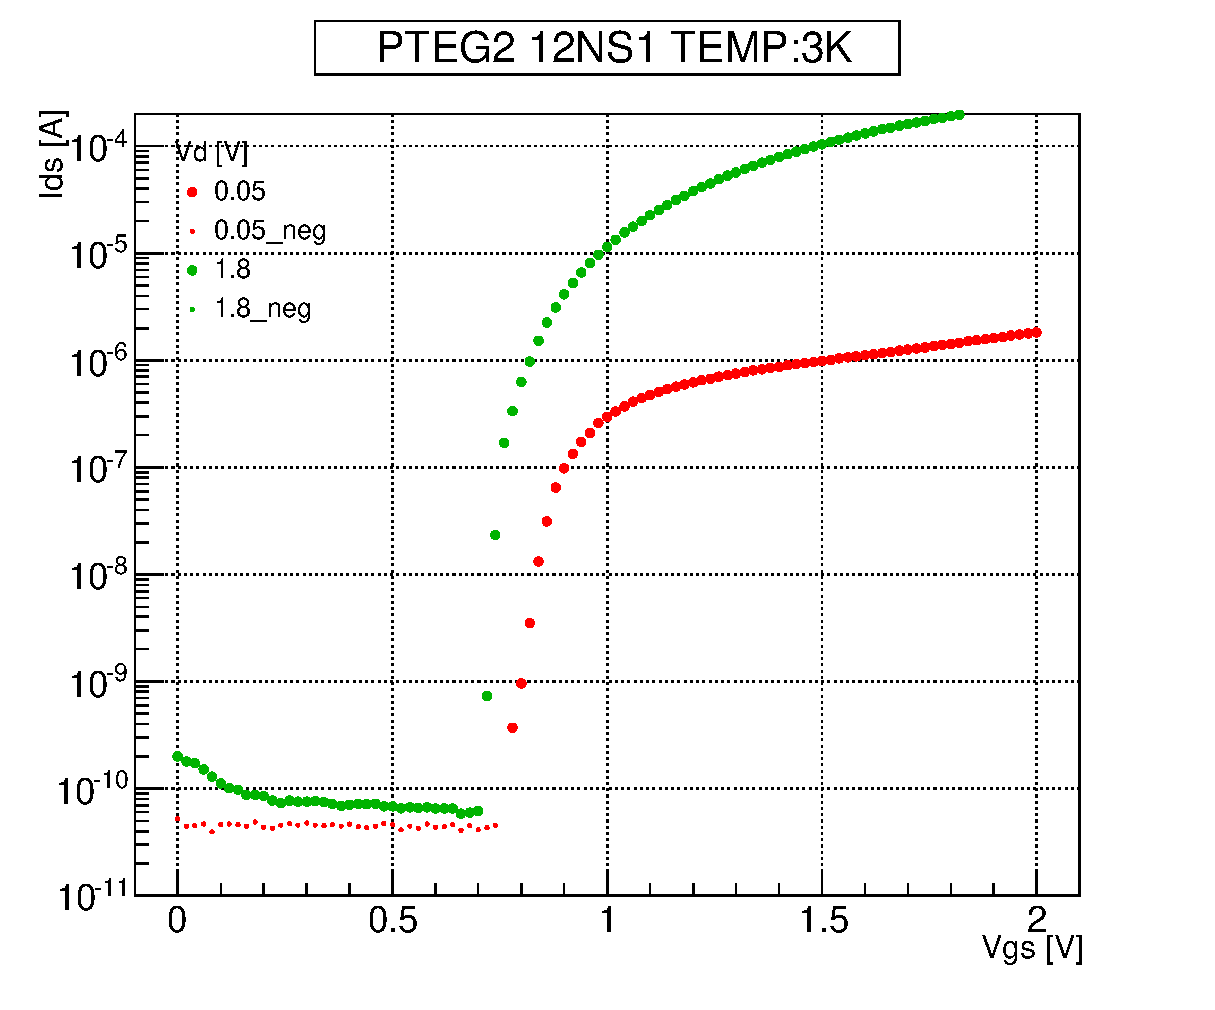
\includegraphics[width=70mm]{./Chapter/Appendix/Picture/NST/NS1/PTEG2_12_NS1_IdVg_3K.eps}
						\end{center}
						\caption{NS1(W/L=$0.4\mathrm{\mu m}/1\mathrm{\mu m}$)の$I_{ds}-V_{gs}$特性(3K)}
						\label{fig:NS1_IdVg_3K}
					\end{minipage}
					\begin{minipage}{0.5\hsize}
						\begin{center}
							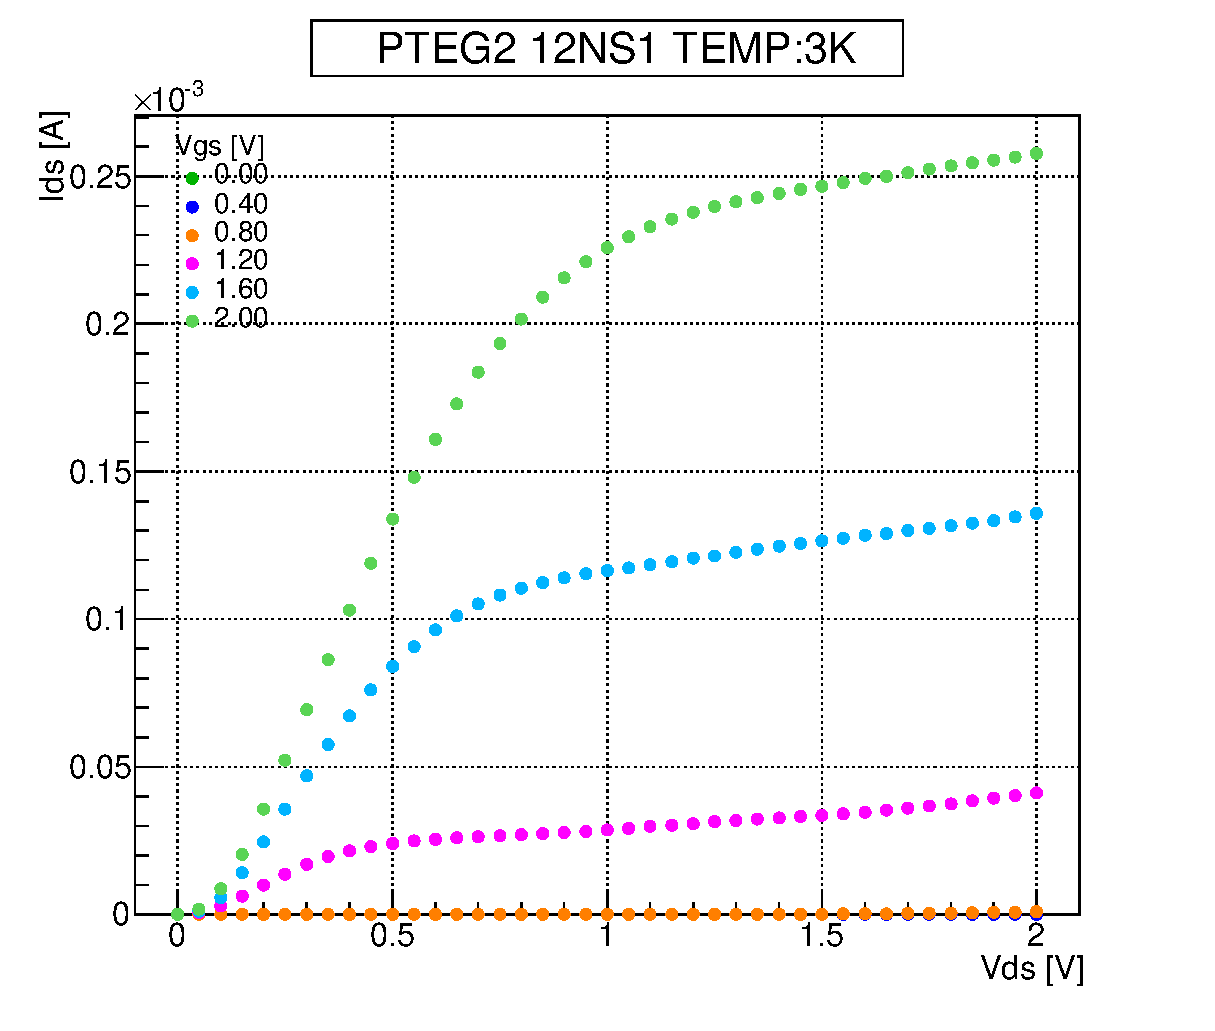
\includegraphics[width=70mm]{./Chapter/Appendix/Picture/NST/NS1/PTEG2_12_NS1_IdVd_3K.eps}
						\end{center}
						\caption{NS1(W/L=$0.4\mathrm{\mu m}/1\mathrm{\mu m}$)の$I_{ds}-V_{ds}$特性(3K)}
						\label{fig:NS1_IdVd_3K}
					\end{minipage}
				\end{figure}
				%=====NS2=====%
				\begin{figure}[htbp]
					\begin{minipage}{0.5\hsize}
						\begin{center}
							\includegraphics[width=70mm]{./Chapter/Appendix/Picture/NST/NS2/PTEG2_12_NS2_IdVg_3K.eps}
						\end{center}
						\caption{NS2(W/L=$0.4\mathrm{\mu m}/2\mathrm{\mu m}$)の$I_{ds}-V_{gs}$特性(3K)}
						\label{fig:NS2_IdVg_3K}
					\end{minipage}
					\begin{minipage}{0.5\hsize}
						\begin{center}
							\includegraphics[width=70mm]{./Chapter/Appendix/Picture/NST/NS2/PTEG2_12_NS2_IdVd_3K.eps}
						\end{center}
						\caption{NS2(W/L=$0.4\mathrm{\mu m}/2\mathrm{\mu m}$)の$I_{ds}-V_{ds}$特性(3K)}
						\label{fig:NS2_IdVd_3K}
					\end{minipage}
				\end{figure}
				%=====NS3=====%
				\begin{figure}[htbp]
					\begin{minipage}{0.5\hsize}
						\begin{center}
							\includegraphics[width=70mm]{./Chapter/Appendix/Picture/NST/NS3/PTEG2_12_NS3_IdVg_3K.eps}
						\end{center}
						\caption{NS3(W/L=$0.4\mathrm{\mu m}/10\mathrm{\mu m}$)の$I_{ds}-V_{gs}$特性(3K)}
						\label{fig:NS3_IdVg_3K}
					\end{minipage}
					\begin{minipage}{0.5\hsize}
						\begin{center}
							\includegraphics[width=70mm]{./Chapter/Appendix/Picture/NST/NS3/PTEG2_12_NS3_IdVd_3K.eps}
						\end{center}
						\caption{NS3(W/L=$0.4\mathrm{\mu m}/10\mathrm{\mu m}$)の$I_{ds}-V_{ds}$特性(3K)}
						\label{fig:NS3_IdVd_3K}
					\end{minipage}
				\end{figure}
				%=====NS4=====%
				\begin{figure}[htbp]
					\begin{minipage}{0.5\hsize}
						\begin{center}
							\includegraphics[width=70mm]{./Chapter/Appendix/Picture/NST/NS4/PTEG2_10_NS4_IdVg_3K.eps}
						\end{center}
						\caption{NS4(W/L=$1\mathrm{\mu m}/10\mathrm{\mu m}$)の$I_{ds}-V_{gs}$特性(3K)}
						\label{fig:NS4_IdVg_3K}
					\end{minipage}
					\begin{minipage}{0.5\hsize}
						\begin{center}
							\includegraphics[width=70mm]{./Chapter/Appendix/Picture/NST/NS4/PTEG2_10_NS4_IdVd_3K.eps}
						\end{center}
						\caption{NS4(W/L=$0.4\mathrm{\mu m}/10\mathrm{\mu m}$)の$I_{ds}-V_{ds}$特性(3K)}
						\label{fig:NS4_IdVd_3K}
					\end{minipage}
				\end{figure}
				%=====NS5=====%
				\begin{figure}[htbp]
					\begin{minipage}{0.5\hsize}
						\begin{center}
							\includegraphics[width=70mm]{./Chapter/Appendix/Picture/NST/NS5/PTEG2_11_NS5_IdVg_3K_2.eps}
						\end{center}
						\caption{NS5(W/L=$5\mathrm{\mu m}/10\mathrm{\mu m}$)の$I_{ds}-V_{gs}$特性(3K)}
						\label{fig:NS5_IdVg_3K}
					\end{minipage}
					\begin{minipage}{0.5\hsize}
						\begin{center}
							\includegraphics[width=70mm]{./Chapter/Appendix/Picture/NST/NS5/PTEG2_11_NS5_IdVd_3K_2.eps}
						\end{center}
						\caption{NS5(W/L=$5\mathrm{\mu m}/10\mathrm{\mu m}$)の$I_{ds}-V_{ds}$特性(3K)}
						\label{fig:NS5_IdVd_3K}
					\end{minipage}
				\end{figure}
				%=====NS6=====%
				\begin{figure}[htbp]
					\begin{minipage}{0.5\hsize}
						\begin{center}
							\includegraphics[width=70mm]{./Chapter/Appendix/Picture/NST/NS6/PTEG2_10_NS6_IdVg_3K.eps}
						\end{center}
						\caption{NS6(W/L=$1\mathrm{\mu m}/1\mathrm{\mu m}$)の$I_{ds}-V_{gs}$特性(3K)}
						\label{fig:NS6_IdVg_3K}
					\end{minipage}
					\begin{minipage}{0.5\hsize}
						\begin{center}
							\includegraphics[width=70mm]{./Chapter/Appendix/Picture/NST/NS6/PTEG2_10_NS6_IdVd_3K.eps}
						\end{center}
						\caption{NS6(W/L=$1\mathrm{\mu m}/1\mathrm{\mu m}$)の$I_{ds}-V_{ds}$特性(3K)}
						\label{fig:NS6_IdVd_3K}
					\end{minipage}
				\end{figure}
				%=====NS7=====%
				\begin{figure}[htbp]
					\begin{minipage}{0.5\hsize}
						\begin{center}
							\includegraphics[width=70mm]{./Chapter/Appendix/Picture/NST/NS7/PTEG2_12_NS7_IdVg_3K.eps}
						\end{center}
						\caption{NS7(W/L=$5\mathrm{\mu m}/1\mathrm{\mu m}$)の$I_{ds}-V_{gs}$特性(3K)}
						\label{fig:NS7_IdVg_3K}
					\end{minipage}
					\begin{minipage}{0.5\hsize}
						\begin{center}
							\includegraphics[width=70mm]{./Chapter/Appendix/Picture/NST/NS7/PTEG2_12_NS7_IdVd_3K.eps}
						\end{center}
						\caption{NS7(W/L=$5\mathrm{\mu m}/1\mathrm{\mu m}$)の$I_{ds}-V_{ds}$特性(3K)}
						\label{fig:NS7_IdVd_3K}
					\end{minipage}
				\end{figure}
				%=====NS8=====%
				\begin{figure}[htbp]
					\begin{minipage}{0.5\hsize}
						\begin{center}
							\includegraphics[width=70mm]{./Chapter/Appendix/Picture/NST/NS8/PTEG2_12_NS8_IdVg_3K.eps}
						\end{center}
						\caption{NS8(W/L=$1\mathrm{\mu m}/2\mathrm{\mu m}$)の$I_{ds}-V_{gs}$特性(3K)}
						\label{fig:NS8_IdVg_3K}
					\end{minipage}
					\begin{minipage}{0.5\hsize}
						\begin{center}
							\includegraphics[width=70mm]{./Chapter/Appendix/Picture/NST/NS8/PTEG2_12_NS8_IdVd_3K.eps}
						\end{center}
						\caption{NS8(W/L=$1\mathrm{\mu m}/2\mathrm{\mu m}$)の$I_{ds}-V_{ds}$特性(3K)}
						\label{fig:NS8_IdVd_3K}
					\end{minipage}
				\end{figure}
				\clearpage
		
		\section{PMOS-ST2(常温環境)}
				%=====PS1=====%
				\begin{figure}[htbp]
					\begin{minipage}{0.5\hsize}
						\begin{center}
							\includegraphics[width=70mm]{./Chapter/Appendix/Picture/PST/PS1/PTEG2_10_PS1_IdVg_rmsetFL.eps}
						\end{center}
						\caption{PS1(W/L=$0.4\mathrm{\mu m}/1\mathrm{\mu m}$)の$I_{ds}-V_{gs}$特性(常温)}
						\label{fig:PS1_IdVg_room}
					\end{minipage}
					\begin{minipage}{0.5\hsize}
						\begin{center}
							\includegraphics[width=70mm]{./Chapter/Appendix/Picture/PST/PS1/PTEG2_10_PS1_IdVd_rmsetFL.eps}
						\end{center}
						\caption{PS1(W/L=$0.4\mathrm{\mu m}/1\mathrm{\mu m}$)の$I_{ds}-V_{ds}$特性(常温)}
						\label{fig:PS1_IdVd_room}
					\end{minipage}
				\end{figure}
				%=====PS2=====%
				\begin{figure}[htbp]
					\begin{minipage}{0.5\hsize}
						\begin{center}
							\includegraphics[width=70mm]{./Chapter/Appendix/Picture/PST/PS2/PTEG2_10_PS2_IdVg_rmsetFL.eps}
						\end{center}
						\caption{PS2(W/L=$0.4\mathrm{\mu m}/2\mathrm{\mu m}$)の$I_{ds}-V_{gs}$特性(常温)}
						\label{fig:PS2_IdVg_room}
					\end{minipage}
					\begin{minipage}{0.5\hsize}
						\begin{center}
							\includegraphics[width=70mm]{./Chapter/Appendix/Picture/PST/PS2/PTEG2_10_PS2_IdVd_rmsetFL.eps}
						\end{center}
						\caption{PS2(W/L=$0.4\mathrm{\mu m}/2\mathrm{\mu m}$)の$I_{ds}-V_{ds}$特性(常温)}
						\label{fig:PS2_IdVd_room}
					\end{minipage}
				\end{figure}
				%=====PS3=====%
				\begin{figure}[htbp]
					\begin{minipage}{0.5\hsize}
						\begin{center}
							\includegraphics[width=70mm]{./Chapter/Appendix/Picture/PST/PS3/PTEG2_10_PS3_IdVg_roomset.eps}
						\end{center}
						\caption{PS3(W/L=$0.4\mathrm{\mu m}/10\mathrm{\mu m}$)の$I_{ds}-V_{gs}$特性(常温)}
						\label{fig:PS3_IdVg_room}
					\end{minipage}
					\begin{minipage}{0.5\hsize}
						\begin{center}
							\includegraphics[width=70mm]{./Chapter/Appendix/Picture/PST/PS3/PTEG2_10_PS3_IdVd_roomset.eps}
						\end{center}
						\caption{PS3(W/L=$0.4\mathrm{\mu m}/10\mathrm{\mu m}$)の$I_{ds}-V_{ds}$特性(常温)}
						\label{fig:PS3_IdVd_room}
					\end{minipage}
				\end{figure}
				%=====PS4=====%
				\begin{figure}[htbp]
					\begin{minipage}{0.5\hsize}
						\begin{center}
							\includegraphics[width=70mm]{./Chapter/Appendix/Picture/PST/PS4/PTEG2_11_PS4_IdVg_roomset2.eps}
						\end{center}
						\caption{PS4(W/L=$1\mathrm{\mu m}/10\mathrm{\mu m}$)の$I_{ds}-V_{gs}$特性(常温)}
						\label{fig:PS4_IdVg_room}
					\end{minipage}
					\begin{minipage}{0.5\hsize}
						\begin{center}
							\includegraphics[width=70mm]{./Chapter/Appendix/Picture/PST/PS4/PTEG2_11_PS4_IdVd_roomset2.eps}
						\end{center}
						\caption{PS4(W/L=$0.4\mathrm{\mu m}/10\mathrm{\mu m}$)の$I_{ds}-V_{ds}$特性(常温)}
						\label{fig:PS4_IdVd_room}
					\end{minipage}
				\end{figure}
				%=====PS5=====%
				\begin{figure}[htbp]
					\begin{minipage}{0.5\hsize}
						\begin{center}
							\includegraphics[width=70mm]{./Chapter/Appendix/Picture/PST/PS5/PTEG2_11_PS5_IdVg_roomset2.eps}
						\end{center}
						\caption{PS5(W/L=$5\mathrm{\mu m}/10\mathrm{\mu m}$)の$I_{ds}-V_{gs}$特性(常温)}
						\label{fig:PS5_IdVg_room}
					\end{minipage}
					\begin{minipage}{0.5\hsize}
						\begin{center}
							\includegraphics[width=70mm]{./Chapter/Appendix/Picture/PST/PS5/PTEG2_11_PS5_IdVd_roomset2.eps}
						\end{center}
						\caption{PS5(W/L=$5\mathrm{\mu m}/10\mathrm{\mu m}$)の$I_{ds}-V_{ds}$特性(常温)}
						\label{fig:PS5_IdVd_room}
					\end{minipage}
				\end{figure}
				%=====PS6=====%
				\begin{figure}[htbp]
					\begin{minipage}{0.5\hsize}
						\begin{center}
							\includegraphics[width=70mm]{./Chapter/Appendix/Picture/PST/PS6/PTEG2_11_PS6_IdVg_roomset2.eps}
						\end{center}
						\caption{PS6(W/L=$1\mathrm{\mu m}/1\mathrm{\mu m}$)の$I_{ds}-V_{gs}$特性(常温)}
						\label{fig:PS6_IdVg_room}
					\end{minipage}
					\begin{minipage}{0.5\hsize}
						\begin{center}
							\includegraphics[width=70mm]{./Chapter/Appendix/Picture/PST/PS6/PTEG2_11_PS6_IdVd_roomset2.eps}
						\end{center}
						\caption{PS6(W/L=$1\mathrm{\mu m}/1\mathrm{\mu m}$)の$I_{ds}-V_{ds}$特性(常温)}
						\label{fig:PS6_IdVd_room}
					\end{minipage}
				\end{figure}
				%=====PS7=====%
				\begin{figure}[htbp]
					\begin{minipage}{0.5\hsize}
						\begin{center}
							\includegraphics[width=70mm]{./Chapter/Appendix/Picture/PST/PS7/PTEG2_11_PS7_IdVg_roomset2.eps}
						\end{center}
						\caption{PS7(W/L=$5\mathrm{\mu m}/1\mathrm{\mu m}$)の$I_{ds}-V_{gs}$特性(常温)}
						\label{fig:PS7_IdVg_room}
					\end{minipage}
					\begin{minipage}{0.5\hsize}
						\begin{center}
							\includegraphics[width=70mm]{./Chapter/Appendix/Picture/PST/PS7/PTEG2_11_PS7_IdVd_roomset2.eps}
						\end{center}
						\caption{PS7(W/L=$5\mathrm{\mu m}/1\mathrm{\mu m}$)の$I_{ds}-V_{ds}$特性(常温)}
						\label{fig:PS7_IdVd_room}
					\end{minipage}
				\end{figure}
				%=====PS8=====%
				\begin{figure}[htbp]
					\begin{minipage}{0.5\hsize}
						\begin{center}
							\includegraphics[width=70mm]{./Chapter/Appendix/Picture/PST/PS8/PTEG2_11_PS8_IdVg_roomset2.eps}
						\end{center}
						\caption{PS8(W/L=$1\mathrm{\mu m}/2\mathrm{\mu m}$)の$I_{ds}-V_{gs}$特性(常温)}
						\label{fig:PS8_IdVg_room}
					\end{minipage}
					\begin{minipage}{0.5\hsize}
						\begin{center}
							\includegraphics[width=70mm]{./Chapter/Appendix/Picture/PST/PS8/PTEG2_11_PS8_IdVd_roomset2.eps}
						\end{center}
						\caption{PS8(W/L=$1\mathrm{\mu m}/2\mathrm{\mu m}$)の$I_{ds}-V_{ds}$特性(常温)}
						\label{fig:PS8_IdVd_room}
					\end{minipage}
				\end{figure}
				\clearpage
		
		\section{PMOS-ST2(3K環境)}
			%=====PS1=====%
				\begin{figure}[htbp]
					\begin{minipage}{0.5\hsize}
						\begin{center}
							\includegraphics[width=70mm]{./Chapter/Appendix/Picture/PST/PS1/PTEG2_10_PS1_IdVg_3K.eps}
						\end{center}
						\caption{PS1(W/L=$0.4\mathrm{\mu m}/1\mathrm{\mu m}$)の$I_{ds}-V_{gs}$特性(3K)}
						\label{fig:PS1_IdVg_3K}
					\end{minipage}
					\begin{minipage}{0.5\hsize}
						\begin{center}
							\includegraphics[width=70mm]{./Chapter/Appendix/Picture/PST/PS1/PTEG2_10_PS1_IdVd_3K.eps}
						\end{center}
						\caption{PS1(W/L=$0.4\mathrm{\mu m}/1\mathrm{\mu m}$)の$I_{ds}-V_{ds}$特性(3K)}
						\label{fig:PS1_IdVd_3K}
					\end{minipage}
				\end{figure}
				%=====PS2=====%
				\begin{figure}[htbp]
					\begin{minipage}{0.5\hsize}
						\begin{center}
							\includegraphics[width=70mm]{./Chapter/Appendix/Picture/PST/PS2/PTEG2_10_PS2_IdVg_3K.eps}
						\end{center}
						\caption{PS2(W/L=$0.4\mathrm{\mu m}/2\mathrm{\mu m}$)の$I_{ds}-V_{gs}$特性(常温)}
						\label{fig:PS2_IdVg_3K}
					\end{minipage}
					\begin{minipage}{0.5\hsize}
						\begin{center}
							\includegraphics[width=70mm]{./Chapter/Appendix/Picture/PST/PS2/PTEG2_10_PS2_IdVd_3K.eps}
						\end{center}
						\caption{PS2(W/L=$0.4\mathrm{\mu m}/2\mathrm{\mu m}$)の$I_{ds}-V_{ds}$特性(常温)}
						\label{fig:PS2_IdVd_3K}
					\end{minipage}
				\end{figure}
				%=====PS3=====%
				\begin{figure}[htbp]
					\begin{minipage}{0.5\hsize}
						\begin{center}
							\includegraphics[width=70mm]{./Chapter/Appendix/Picture/PST/PS3/PTEG2_10_PS3_IdVg_3K.eps}
						\end{center}
						\caption{PS3(W/L=$0.4\mathrm{\mu m}/10\mathrm{\mu m}$)の$I_{ds}-V_{gs}$特性(3K)}
						\label{fig:PS3_IdVg_3K}
					\end{minipage}
					\begin{minipage}{0.5\hsize}
						\begin{center}
							\includegraphics[width=70mm]{./Chapter/Appendix/Picture/PST/PS3/PTEG2_10_PS3_IdVd_3K.eps}
						\end{center}
						\caption{PS3(W/L=$0.4\mathrm{\mu m}/10\mathrm{\mu m}$)の$I_{ds}-V_{ds}$特性(3K)}
						\label{fig:PS3_IdVd_3K}
					\end{minipage}
				\end{figure}
				%=====PS4=====%
				\begin{figure}[htbp]
					\begin{minipage}{0.5\hsize}
						\begin{center}
							\includegraphics[width=70mm]{./Chapter/Appendix/Picture/PST/PS4/PTEG2_11_PS4_IdVg_3K.eps}
						\end{center}
						\caption{PS4(W/L=$1\mathrm{\mu m}/10\mathrm{\mu m}$)の$I_{ds}-V_{gs}$特性(3K)}
						\label{fig:PS4_IdVg_3K}
					\end{minipage}
					\begin{minipage}{0.5\hsize}
						\begin{center}
							\includegraphics[width=70mm]{./Chapter/Appendix/Picture/PST/PS4/PTEG2_11_PS4_IdVd_3K.eps}
						\end{center}
						\caption{PS4(W/L=$0.4\mathrm{\mu m}/10\mathrm{\mu m}$)の$I_{ds}-V_{ds}$特性(3K)}
						\label{fig:PS4_IdVd_3K}
					\end{minipage}
				\end{figure}
				%=====PS5=====%
				\begin{figure}[htbp]
					\begin{minipage}{0.5\hsize}
						\begin{center}
							\includegraphics[width=70mm]{./Chapter/Appendix/Picture/PST/PS5/PTEG2_11_PS5_IdVg_3K.eps}
						\end{center}
						\caption{PS5(W/L=$5\mathrm{\mu m}/10\mathrm{\mu m}$)の$I_{ds}-V_{gs}$特性(3K)}
						\label{fig:PS5_IdVg_3K}
					\end{minipage}
					\begin{minipage}{0.5\hsize}
						\begin{center}
							\includegraphics[width=70mm]{./Chapter/Appendix/Picture/PST/PS5/PTEG2_11_PS5_IdVd_3K.eps}
						\end{center}
						\caption{PS5(W/L=$5\mathrm{\mu m}/10\mathrm{\mu m}$)の$I_{ds}-V_{ds}$特性(3K)}
						\label{fig:PS5_IdVd_3K}
					\end{minipage}
				\end{figure}
				%=====PS6=====%
				\begin{figure}[htbp]
					\begin{minipage}{0.5\hsize}
						\begin{center}
							\includegraphics[width=70mm]{./Chapter/Appendix/Picture/PST/PS6/PTEG2_11_PS6_IdVg_3K.eps}
						\end{center}
						\caption{PS6(W/L=$1\mathrm{\mu m}/1\mathrm{\mu m}$)の$I_{ds}-V_{gs}$特性(3K)}
						\label{fig:PS6_IdVg_3K}
					\end{minipage}
					\begin{minipage}{0.5\hsize}
						\begin{center}
							\includegraphics[width=70mm]{./Chapter/Appendix/Picture/PST/PS6/PTEG2_11_PS6_IdVd_3K.eps}
						\end{center}
						\caption{PS6(W/L=$1\mathrm{\mu m}/1\mathrm{\mu m}$)の$I_{ds}-V_{ds}$特性(3K)}
						\label{fig:PS6_IdVd_3K}
					\end{minipage}
				\end{figure}
				%=====PS7=====%
				\begin{figure}[htbp]
					\begin{minipage}{0.5\hsize}
						\begin{center}
							\includegraphics[width=70mm]{./Chapter/Appendix/Picture/PST/PS7/PTEG2_11_PS7_IdVg_3K.eps}
						\end{center}
						\caption{PS7(W/L=$5\mathrm{\mu m}/1\mathrm{\mu m}$)の$I_{ds}-V_{gs}$特性(3K)}
						\label{fig:PS7_IdVg_3K}
					\end{minipage}
					\begin{minipage}{0.5\hsize}
						\begin{center}
							\includegraphics[width=70mm]{./Chapter/Appendix/Picture/PST/PS7/PTEG2_11_PS7_IdVd_3K.eps}
						\end{center}
						\caption{PS7(W/L=$5\mathrm{\mu m}/1\mathrm{\mu m}$)の$I_{ds}-V_{ds}$特性(3K)}
						\label{fig:PS7_IdVd_3K}
					\end{minipage}
				\end{figure}
				%=====PS8=====%
				\begin{figure}[htbp]
					\begin{minipage}{0.5\hsize}
						\begin{center}
							\includegraphics[width=70mm]{./Chapter/Appendix/Picture/PST/PS8/PTEG2_11_PS8_IdVg_3K.eps}
						\end{center}
						\caption{PS8(W/L=$1\mathrm{\mu m}/2\mathrm{\mu m}$)の$I_{ds}-V_{gs}$特性(3K)}
						\label{fig:PS8_IdVg_3K}
					\end{minipage}
					\begin{minipage}{0.5\hsize}
						\begin{center}
							\includegraphics[width=70mm]{./Chapter/Appendix/Picture/PST/PS8/PTEG2_11_PS8_IdVd_3K.eps}
						\end{center}
						\caption{PS8(W/L=$1\mathrm{\mu m}/2\mathrm{\mu m}$)の$I_{ds}-V_{ds}$特性(3K)}
						\label{fig:PS8_IdVd_3K}
					\end{minipage}
				\end{figure}
			\clearpage
	
	
	
	
	
	